\documentclass{article}

% Keep the original numerical citation convention.
\PassOptionsToPackage{numbers,sort,compress}{natbib}
\usepackage{iclr2027_conference,times}

\usepackage[utf8]{inputenc}
\usepackage[T1]{fontenc}
\usepackage{amssymb,amsthm}
\usepackage{multirow}
\usepackage{thm-restate}
\usepackage{algpseudocode,algorithm}
\usepackage{booktabs}
\usepackage{graphicx}
\usepackage{nicefrac}
\usepackage{microtype}
\usepackage{xcolor}
\usepackage{hyperref}
\usepackage{url}

% Mathematical notation retained from the supplied source/template.
%%%%% NEW MATH DEFINITIONS %%%%%

\usepackage{amsmath,amsfonts,bm}

% Mark sections of captions for referring to divisions of figures
\newcommand{\figleft}{{\em (Left)}}
\newcommand{\figcenter}{{\em (Center)}}
\newcommand{\figright}{{\em (Right)}}
\newcommand{\figtop}{{\em (Top)}}
\newcommand{\figbottom}{{\em (Bottom)}}
\newcommand{\captiona}{{\em (a)}}
\newcommand{\captionb}{{\em (b)}}
\newcommand{\captionc}{{\em (c)}}
\newcommand{\captiond}{{\em (d)}}

% Highlight a newly defined term
\newcommand{\newterm}[1]{{\bf #1}}


% Figure reference, lower-case.
\def\figref#1{figure~\ref{#1}}
% Figure reference, capital. For start of sentence
\def\Figref#1{Figure~\ref{#1}}
\def\twofigref#1#2{figures \ref{#1} and \ref{#2}}
\def\quadfigref#1#2#3#4{figures \ref{#1}, \ref{#2}, \ref{#3} and \ref{#4}}
% Section reference, lower-case.
\def\secref#1{section~\ref{#1}}
% Section reference, capital.
\def\Secref#1{Section~\ref{#1}}
% Reference to two sections.
\def\twosecrefs#1#2{sections \ref{#1} and \ref{#2}}
% Reference to three sections.
\def\secrefs#1#2#3{sections \ref{#1}, \ref{#2} and \ref{#3}}
% Reference to an equation, lower-case.
\def\eqref#1{equation~\ref{#1}}
% Reference to an equation, upper case
\def\Eqref#1{Equation~\ref{#1}}
% A raw reference to an equation---avoid using if possible
\def\plaineqref#1{\ref{#1}}
% Reference to a chapter, lower-case.
\def\chapref#1{chapter~\ref{#1}}
% Reference to an equation, upper case.
\def\Chapref#1{Chapter~\ref{#1}}
% Reference to a range of chapters
\def\rangechapref#1#2{chapters\ref{#1}--\ref{#2}}
% Reference to an algorithm, lower-case.
\def\algref#1{algorithm~\ref{#1}}
% Reference to an algorithm, upper case.
\def\Algref#1{Algorithm~\ref{#1}}
\def\twoalgref#1#2{algorithms \ref{#1} and \ref{#2}}
\def\Twoalgref#1#2{Algorithms \ref{#1} and \ref{#2}}
% Reference to a part, lower case
\def\partref#1{part~\ref{#1}}
% Reference to a part, upper case
\def\Partref#1{Part~\ref{#1}}
\def\twopartref#1#2{parts \ref{#1} and \ref{#2}}

\def\ceil#1{\lceil #1 \rceil}
\def\floor#1{\lfloor #1 \rfloor}
\def\1{\bm{1}}
\newcommand{\train}{\mathcal{D}}
\newcommand{\valid}{\mathcal{D_{\mathrm{valid}}}}
\newcommand{\test}{\mathcal{D_{\mathrm{test}}}}

\def\eps{{\epsilon}}


% Random variables
\def\reta{{\textnormal{$\eta$}}}
\def\ra{{\textnormal{a}}}
\def\rb{{\textnormal{b}}}
\def\rc{{\textnormal{c}}}
\def\rd{{\textnormal{d}}}
\def\re{{\textnormal{e}}}
\def\rf{{\textnormal{f}}}
\def\rg{{\textnormal{g}}}
\def\rh{{\textnormal{h}}}
\def\ri{{\textnormal{i}}}
\def\rj{{\textnormal{j}}}
\def\rk{{\textnormal{k}}}
\def\rl{{\textnormal{l}}}
% rm is already a command, just don't name any random variables m
\def\rn{{\textnormal{n}}}
\def\ro{{\textnormal{o}}}
\def\rp{{\textnormal{p}}}
\def\rq{{\textnormal{q}}}
\def\rr{{\textnormal{r}}}
\def\rs{{\textnormal{s}}}
\def\rt{{\textnormal{t}}}
\def\ru{{\textnormal{u}}}
\def\rv{{\textnormal{v}}}
\def\rw{{\textnormal{w}}}
\def\rx{{\textnormal{x}}}
\def\ry{{\textnormal{y}}}
\def\rz{{\textnormal{z}}}

% Random vectors
\def\rvepsilon{{\mathbf{\epsilon}}}
\def\rvtheta{{\mathbf{\theta}}}
\def\rva{{\mathbf{a}}}
\def\rvb{{\mathbf{b}}}
\def\rvc{{\mathbf{c}}}
\def\rvd{{\mathbf{d}}}
\def\rve{{\mathbf{e}}}
\def\rvf{{\mathbf{f}}}
\def\rvg{{\mathbf{g}}}
\def\rvh{{\mathbf{h}}}
\def\rvu{{\mathbf{i}}}
\def\rvj{{\mathbf{j}}}
\def\rvk{{\mathbf{k}}}
\def\rvl{{\mathbf{l}}}
\def\rvm{{\mathbf{m}}}
\def\rvn{{\mathbf{n}}}
\def\rvo{{\mathbf{o}}}
\def\rvp{{\mathbf{p}}}
\def\rvq{{\mathbf{q}}}
\def\rvr{{\mathbf{r}}}
\def\rvs{{\mathbf{s}}}
\def\rvt{{\mathbf{t}}}
\def\rvu{{\mathbf{u}}}
\def\rvv{{\mathbf{v}}}
\def\rvw{{\mathbf{w}}}
\def\rvx{{\mathbf{x}}}
\def\rvy{{\mathbf{y}}}
\def\rvz{{\mathbf{z}}}

% Elements of random vectors
\def\erva{{\textnormal{a}}}
\def\ervb{{\textnormal{b}}}
\def\ervc{{\textnormal{c}}}
\def\ervd{{\textnormal{d}}}
\def\erve{{\textnormal{e}}}
\def\ervf{{\textnormal{f}}}
\def\ervg{{\textnormal{g}}}
\def\ervh{{\textnormal{h}}}
\def\ervi{{\textnormal{i}}}
\def\ervj{{\textnormal{j}}}
\def\ervk{{\textnormal{k}}}
\def\ervl{{\textnormal{l}}}
\def\ervm{{\textnormal{m}}}
\def\ervn{{\textnormal{n}}}
\def\ervo{{\textnormal{o}}}
\def\ervp{{\textnormal{p}}}
\def\ervq{{\textnormal{q}}}
\def\ervr{{\textnormal{r}}}
\def\ervs{{\textnormal{s}}}
\def\ervt{{\textnormal{t}}}
\def\ervu{{\textnormal{u}}}
\def\ervv{{\textnormal{v}}}
\def\ervw{{\textnormal{w}}}
\def\ervx{{\textnormal{x}}}
\def\ervy{{\textnormal{y}}}
\def\ervz{{\textnormal{z}}}

% Random matrices
\def\rmA{{\mathbf{A}}}
\def\rmB{{\mathbf{B}}}
\def\rmC{{\mathbf{C}}}
\def\rmD{{\mathbf{D}}}
\def\rmE{{\mathbf{E}}}
\def\rmF{{\mathbf{F}}}
\def\rmG{{\mathbf{G}}}
\def\rmH{{\mathbf{H}}}
\def\rmI{{\mathbf{I}}}
\def\rmJ{{\mathbf{J}}}
\def\rmK{{\mathbf{K}}}
\def\rmL{{\mathbf{L}}}
\def\rmM{{\mathbf{M}}}
\def\rmN{{\mathbf{N}}}
\def\rmO{{\mathbf{O}}}
\def\rmP{{\mathbf{P}}}
\def\rmQ{{\mathbf{Q}}}
\def\rmR{{\mathbf{R}}}
\def\rmS{{\mathbf{S}}}
\def\rmT{{\mathbf{T}}}
\def\rmU{{\mathbf{U}}}
\def\rmV{{\mathbf{V}}}
\def\rmW{{\mathbf{W}}}
\def\rmX{{\mathbf{X}}}
\def\rmY{{\mathbf{Y}}}
\def\rmZ{{\mathbf{Z}}}

% Elements of random matrices
\def\ermA{{\textnormal{A}}}
\def\ermB{{\textnormal{B}}}
\def\ermC{{\textnormal{C}}}
\def\ermD{{\textnormal{D}}}
\def\ermE{{\textnormal{E}}}
\def\ermF{{\textnormal{F}}}
\def\ermG{{\textnormal{G}}}
\def\ermH{{\textnormal{H}}}
\def\ermI{{\textnormal{I}}}
\def\ermJ{{\textnormal{J}}}
\def\ermK{{\textnormal{K}}}
\def\ermL{{\textnormal{L}}}
\def\ermM{{\textnormal{M}}}
\def\ermN{{\textnormal{N}}}
\def\ermO{{\textnormal{O}}}
\def\ermP{{\textnormal{P}}}
\def\ermQ{{\textnormal{Q}}}
\def\ermR{{\textnormal{R}}}
\def\ermS{{\textnormal{S}}}
\def\ermT{{\textnormal{T}}}
\def\ermU{{\textnormal{U}}}
\def\ermV{{\textnormal{V}}}
\def\ermW{{\textnormal{W}}}
\def\ermX{{\textnormal{X}}}
\def\ermY{{\textnormal{Y}}}
\def\ermZ{{\textnormal{Z}}}

% Vectors
\def\vzero{{\bm{0}}}
\def\vone{{\bm{1}}}
\def\vmu{{\bm{\mu}}}
\def\vtheta{{\bm{\theta}}}
\def\va{{\bm{a}}}
\def\vb{{\bm{b}}}
\def\vc{{\bm{c}}}
\def\vd{{\bm{d}}}
\def\ve{{\bm{e}}}
\def\vf{{\bm{f}}}
\def\vg{{\bm{g}}}
\def\vh{{\bm{h}}}
\def\vi{{\bm{i}}}
\def\vj{{\bm{j}}}
\def\vk{{\bm{k}}}
\def\vl{{\bm{l}}}
\def\vm{{\bm{m}}}
\def\vn{{\bm{n}}}
\def\vo{{\bm{o}}}
\def\vp{{\bm{p}}}
\def\vq{{\bm{q}}}
\def\vr{{\bm{r}}}
\def\vs{{\bm{s}}}
\def\vt{{\bm{t}}}
\def\vu{{\bm{u}}}
\def\vv{{\bm{v}}}
\def\vw{{\bm{w}}}
\def\vx{{\bm{x}}}
\def\vy{{\bm{y}}}
\def\vz{{\bm{z}}}

% Elements of vectors
\def\evalpha{{\alpha}}
\def\evbeta{{\beta}}
\def\evepsilon{{\epsilon}}
\def\evlambda{{\lambda}}
\def\evomega{{\omega}}
\def\evmu{{\mu}}
\def\evpsi{{\psi}}
\def\evsigma{{\sigma}}
\def\evtheta{{\theta}}
\def\eva{{a}}
\def\evb{{b}}
\def\evc{{c}}
\def\evd{{d}}
\def\eve{{e}}
\def\evf{{f}}
\def\evg{{g}}
\def\evh{{h}}
\def\evi{{i}}
\def\evj{{j}}
\def\evk{{k}}
\def\evl{{l}}
\def\evm{{m}}
\def\evn{{n}}
\def\evo{{o}}
\def\evp{{p}}
\def\evq{{q}}
\def\evr{{r}}
\def\evs{{s}}
\def\evt{{t}}
\def\evu{{u}}
\def\evv{{v}}
\def\evw{{w}}
\def\evx{{x}}
\def\evy{{y}}
\def\evz{{z}}

% Matrix
\def\mA{{\bm{A}}}
\def\mB{{\bm{B}}}
\def\mC{{\bm{C}}}
\def\mD{{\bm{D}}}
\def\mE{{\bm{E}}}
\def\mF{{\bm{F}}}
\def\mG{{\bm{G}}}
\def\mH{{\bm{H}}}
\def\mI{{\bm{I}}}
\def\mJ{{\bm{J}}}
\def\mK{{\bm{K}}}
\def\mL{{\bm{L}}}
\def\mM{{\bm{M}}}
\def\mN{{\bm{N}}}
\def\mO{{\bm{O}}}
\def\mP{{\bm{P}}}
\def\mQ{{\bm{Q}}}
\def\mR{{\bm{R}}}
\def\mS{{\bm{S}}}
\def\mT{{\bm{T}}}
\def\mU{{\bm{U}}}
\def\mV{{\bm{V}}}
\def\mW{{\bm{W}}}
\def\mX{{\bm{X}}}
\def\mY{{\bm{Y}}}
\def\mZ{{\bm{Z}}}
\def\mBeta{{\bm{\beta}}}
\def\mPhi{{\bm{\Phi}}}
\def\mLambda{{\bm{\Lambda}}}
\def\mSigma{{\bm{\Sigma}}}

% Tensor
\DeclareMathAlphabet{\mathsfit}{\encodingdefault}{\sfdefault}{m}{sl}
\SetMathAlphabet{\mathsfit}{bold}{\encodingdefault}{\sfdefault}{bx}{n}
\newcommand{\tens}[1]{\bm{\mathsfit{#1}}}
\def\tA{{\tens{A}}}
\def\tB{{\tens{B}}}
\def\tC{{\tens{C}}}
\def\tD{{\tens{D}}}
\def\tE{{\tens{E}}}
\def\tF{{\tens{F}}}
\def\tG{{\tens{G}}}
\def\tH{{\tens{H}}}
\def\tI{{\tens{I}}}
\def\tJ{{\tens{J}}}
\def\tK{{\tens{K}}}
\def\tL{{\tens{L}}}
\def\tM{{\tens{M}}}
\def\tN{{\tens{N}}}
\def\tO{{\tens{O}}}
\def\tP{{\tens{P}}}
\def\tQ{{\tens{Q}}}
\def\tR{{\tens{R}}}
\def\tS{{\tens{S}}}
\def\tT{{\tens{T}}}
\def\tU{{\tens{U}}}
\def\tV{{\tens{V}}}
\def\tW{{\tens{W}}}
\def\tX{{\tens{X}}}
\def\tY{{\tens{Y}}}
\def\tZ{{\tens{Z}}}


% Graph
\def\gA{{\mathcal{A}}}
\def\gB{{\mathcal{B}}}
\def\gC{{\mathcal{C}}}
\def\gD{{\mathcal{D}}}
\def\gE{{\mathcal{E}}}
\def\gF{{\mathcal{F}}}
\def\gG{{\mathcal{G}}}
\def\gH{{\mathcal{H}}}
\def\gI{{\mathcal{I}}}
\def\gJ{{\mathcal{J}}}
\def\gK{{\mathcal{K}}}
\def\gL{{\mathcal{L}}}
\def\gM{{\mathcal{M}}}
\def\gN{{\mathcal{N}}}
\def\gO{{\mathcal{O}}}
\def\gP{{\mathcal{P}}}
\def\gQ{{\mathcal{Q}}}
\def\gR{{\mathcal{R}}}
\def\gS{{\mathcal{S}}}
\def\gT{{\mathcal{T}}}
\def\gU{{\mathcal{U}}}
\def\gV{{\mathcal{V}}}
\def\gW{{\mathcal{W}}}
\def\gX{{\mathcal{X}}}
\def\gY{{\mathcal{Y}}}
\def\gZ{{\mathcal{Z}}}

% Sets
\def\sA{{\mathbb{A}}}
\def\sB{{\mathbb{B}}}
\def\sC{{\mathbb{C}}}
\def\sD{{\mathbb{D}}}
% Don't use a set called E, because this would be the same as our symbol
% for expectation.
\def\sF{{\mathbb{F}}}
\def\sG{{\mathbb{G}}}
\def\sH{{\mathbb{H}}}
\def\sI{{\mathbb{I}}}
\def\sJ{{\mathbb{J}}}
\def\sK{{\mathbb{K}}}
\def\sL{{\mathbb{L}}}
\def\sM{{\mathbb{M}}}
\def\sN{{\mathbb{N}}}
\def\sO{{\mathbb{O}}}
\def\sP{{\mathbb{P}}}
\def\sQ{{\mathbb{Q}}}
\def\sR{{\mathbb{R}}}
\def\sS{{\mathbb{S}}}
\def\sT{{\mathbb{T}}}
\def\sU{{\mathbb{U}}}
\def\sV{{\mathbb{V}}}
\def\sW{{\mathbb{W}}}
\def\sX{{\mathbb{X}}}
\def\sY{{\mathbb{Y}}}
\def\sZ{{\mathbb{Z}}}

% Entries of a matrix
\def\emLambda{{\Lambda}}
\def\emA{{A}}
\def\emB{{B}}
\def\emC{{C}}
\def\emD{{D}}
\def\emE{{E}}
\def\emF{{F}}
\def\emG{{G}}
\def\emH{{H}}
\def\emI{{I}}
\def\emJ{{J}}
\def\emK{{K}}
\def\emL{{L}}
\def\emM{{M}}
\def\emN{{N}}
\def\emO{{O}}
\def\emP{{P}}
\def\emQ{{Q}}
\def\emR{{R}}
\def\emS{{S}}
\def\emT{{T}}
\def\emU{{U}}
\def\emV{{V}}
\def\emW{{W}}
\def\emX{{X}}
\def\emY{{Y}}
\def\emZ{{Z}}
\def\emSigma{{\Sigma}}

% entries of a tensor
% Same font as tensor, without \bm wrapper
\newcommand{\etens}[1]{\mathsfit{#1}}
\def\etLambda{{\etens{\Lambda}}}
\def\etA{{\etens{A}}}
\def\etB{{\etens{B}}}
\def\etC{{\etens{C}}}
\def\etD{{\etens{D}}}
\def\etE{{\etens{E}}}
\def\etF{{\etens{F}}}
\def\etG{{\etens{G}}}
\def\etH{{\etens{H}}}
\def\etI{{\etens{I}}}
\def\etJ{{\etens{J}}}
\def\etK{{\etens{K}}}
\def\etL{{\etens{L}}}
\def\etM{{\etens{M}}}
\def\etN{{\etens{N}}}
\def\etO{{\etens{O}}}
\def\etP{{\etens{P}}}
\def\etQ{{\etens{Q}}}
\def\etR{{\etens{R}}}
\def\etS{{\etens{S}}}
\def\etT{{\etens{T}}}
\def\etU{{\etens{U}}}
\def\etV{{\etens{V}}}
\def\etW{{\etens{W}}}
\def\etX{{\etens{X}}}
\def\etY{{\etens{Y}}}
\def\etZ{{\etens{Z}}}

% The true underlying data generating distribution
\newcommand{\pdata}{p_{\rm{data}}}
% The empirical distribution defined by the training set
\newcommand{\ptrain}{\hat{p}_{\rm{data}}}
\newcommand{\Ptrain}{\hat{P}_{\rm{data}}}
% The model distribution
\newcommand{\pmodel}{p_{\rm{model}}}
\newcommand{\Pmodel}{P_{\rm{model}}}
\newcommand{\ptildemodel}{\tilde{p}_{\rm{model}}}
% Stochastic autoencoder distributions
\newcommand{\pencode}{p_{\rm{encoder}}}
\newcommand{\pdecode}{p_{\rm{decoder}}}
\newcommand{\precons}{p_{\rm{reconstruct}}}

\newcommand{\laplace}{\mathrm{Laplace}} % Laplace distribution

\newcommand{\E}{\mathbb{E}}
\newcommand{\Ls}{\mathcal{L}}
\newcommand{\R}{\mathbb{R}}
\newcommand{\emp}{\tilde{p}}
\newcommand{\lr}{\alpha}
\newcommand{\reg}{\lambda}
\newcommand{\rect}{\mathrm{rectifier}}
\newcommand{\softmax}{\mathrm{softmax}}
\newcommand{\sigmoid}{\sigma}
\newcommand{\softplus}{\zeta}
\newcommand{\KL}{D_{\mathrm{KL}}}
\newcommand{\Var}{\mathrm{Var}}
\newcommand{\standarderror}{\mathrm{SE}}
\newcommand{\Cov}{\mathrm{Cov}}
% Wolfram Mathworld says $L^2$ is for function spaces and $\ell^2$ is for vectors
% But then they seem to use $L^2$ for vectors throughout the site, and so does
% wikipedia.
\newcommand{\normlzero}{L^0}
\newcommand{\normlone}{L^1}
\newcommand{\normltwo}{L^2}
\newcommand{\normlp}{L^p}
\newcommand{\normmax}{L^\infty}

\newcommand{\parents}{Pa} % See usage in notation.tex. Chosen to match Daphne's book.

\DeclareMathOperator*{\argmax}{arg\,max}
\DeclareMathOperator*{\argmin}{arg\,min}

\DeclareMathOperator{\sign}{sign}
\DeclareMathOperator{\Tr}{Tr}
\let\ab\allowbreak

% Additional notation used by the original NOG source.
\def\vDelta{{\bm{\Delta}}}

% Independent section-based counters preserve the original numbering,
% e.g., Proposition 3.1, Lemma 4.3, and Theorem 4.1.
\newtheorem{thm}{Theorem}[section]
\newtheorem{lem}{Lemma}[section]
\newtheorem{prop}{Proposition}[section]
\newtheorem{fact}{Fact}[section]
\newtheorem{cor}{Corollary}[section]
\theoremstyle{definition}
\newtheorem{dfn}{Definition}[section]
\newtheorem{asm}{Assumption}[section]
\theoremstyle{remark}
\newtheorem{rmk}{Remark}[section]

\title{Highly-Parallel Algorithms for Non-Smooth Non-Convex Optimization}

% Authors remain anonymous in the submission version.
\author{Anonymous Authors}

% Uncomment only for the camera-ready version.
% \iclrfinalcopy
\begin{document}
	
	\maketitle
	
	
	\begin{abstract}
		Recent progress in nonsmooth nonconvex optimization established non-asymptotic convergence to $(\delta,\epsilon)$-Goldstein stationary points with zeroth- or first-order oracles. In this paper, we study the extensions of these results in the parallel setting. We propose a algorithm called Optimistic Nonconvex Gradient (NOG) that can find a $(\delta,\epsilon)$-Goldstein stationary point in $\gO(d^{1/3} \delta^{-1} \epsilon^{-5/3})$ rounds of interactions of the oracles, which strictly improve the one of $\gO(\delta^{-1} \epsilon^{-3})$ given by prior arts when $d = \gO(\epsilon^{-4})$. We further implement our method in
		the distributed and quantum optimization settings, obtaining efficient distributed algorithms in both communication and computation, and fast quantum algorithms in quantum oracle query complexities.
	\end{abstract}
	
	\section{Introduction}
	
	This paper studies the stochastic optimization problem of the form
	\begin{align} \label{prob:main}
		\min_{\vx \in \sR^d} f(\vx) \triangleq \mathbb{E}_{\xi \in \Xi} [F(\vx; \xi)],
	\end{align}
	where the stochastic component $F(\vx;\xi)$, indexed by random variable $\xi$ defined on the data distribution $\Xi$, is possibly nonconvex and nonsmooth. This nonsmooth nonconvex optimization covers a lot of applications in statistics \citep{fan2001variable,zhang2010analysis}, economics \citep{duffie2010dynamic,stadtler2014supply}, and deep learning \citep{lecun2015deep,davis2020stochastic,bolte2021conservative,zhang2020complexity}. 
	
	% In 2020, 
	
	For nonsmooth nonconvex optimization,
	\citet{zhang2020complexity} showed traditional $\epsilon$-stationary point cannot be obtained in finite time and proposed the Stochastic Interpolated Normalized Gradient Descent (SINGD) that can provably find a $(\delta,\epsilon)$-Goldstein stationary point \citep{goldstein1977optimization} in $\gO(\delta^{-1} \epsilon^{-4})$ stochastic first-order oracle (SFO) complexity. 
	\citet{cutkosky2023optimal} proposed optimal first-order  methods with $\gO(\delta^{-1} \epsilon^{-3})$ SFO complexity via a novel Online-to-Nonconvex Conversion (O2NC). \citet{kornowski2024algorithm} showed a zeroth-order implementation of O2NC with two-point gradient estimator \citep{shamir2017optimal,duchi2015optimal} achieves a  $\gO(d \delta^{-1} \epsilon^{-3})$ stochastic zeroth-order oracle (SZO) complexity.
	
	% \citet{kornowski2024algorithm} proposed a zeroth-order implementation achieving xxx.
	% While first- and zeroth-order methods for nonsmooth nonconvex optimization have been extensively studied, 
	
	Although optimal first-order \citep{cutkosky2023optimal} and optimal dimension-dependent zeroth-order methods \citep{kornowski2024algorithm} have been proposed, these methods are studied under the sequential setting. 
	With the growing size of training datasets, modern training often relies on parallel computing resources like GPUs and TPUs. To capture this scenario, we 
	consider the parallel setting, where the algorithm can simultaneously submit multiple queries $\{(\vx_1,\xi_1),\cdots, (\vx_Q,\xi_Q) \}$ at once, and then the zeroth- or first-order oracles return the function values or gradients at these points to the algorithm. Following the work by \citet{nemirovski1994parallel}, the complexity of a parallel algorithm is measured by both \textit{depth} (the number of rounds the algorithm interact with the oracles) and \textit{work} (the total number of queries, \textit{i.e.}, $Q \times$ depth). This work tries to answer the following fundamental question:
	\begin{center}
		\textit{Can we develop fast parallel algorithms for nonsmooth nonconvex optimization?}
	\end{center}
	Although there have been many works studying the complexity of parallel algorithms for convex problems \citep{duchi2012randomized,bubeck2019complexity,diakonikolas2019lower,balkanski2018parallelization,jambulapati2024closing,carmon2023resqueing,scaman2018optimal,garg2020no,garg2021near,sidford2023quantum} or smooth nonconvex problems \citep{zhang2023quantum,zhou2025adaptive}, the power of parallelism in nonsmooth nonconvex optimization is less explored. 
	To fill the gap, this work extends the randomized smoothing techniques in \citet{duchi2012randomized} for nonsmooth convex problems to nonsmooth nonconvex problems, and proposes a novel Nonconvex Optimistic Gradient (NOG) method that achieves a low depth of $\gO(d^{1/3} \delta^{-1} \epsilon^{-5/3})$ for finding a $(\delta,\epsilon)$-Goldstein stationary point. The depth of our method improves the $\gO(\delta^{-1} \epsilon^{-3})$ of O2NC \citep{cutkosky2023optimal,kornowski2024algorithm} and the $\gO(\sqrt{d} \delta^{-1} \epsilon^{-2})$ of naive gradient descent with randomized smoothing \citep{lin2022gradient,jordan2023deterministic,chen2023faster}, and the total work of our method aligns with the state-of-the-art ones obtained by O2NC \citep{cutkosky2023optimal,kornowski2024algorithm} when using either first- or zeroth-order oracles, \textit{i.e.}, $\gO(\delta^{-1} \epsilon^{-3} )$ SFO complexity and $\gO(d \delta^{-1} \epsilon^{-3})$ SZO complexity. 
	We compare the theoretical guarantee of the proposed NOG  with previous ones in Table~\ref{tab:res-classical}.
	
	Our algorithm is well-suited for various scenarios requiring high parallelism. A natural application is distributed optimization, where multiple parallel workers collaborate to perform optimization tasks. The complexity of a distributed algorithm is typically measured by communication and computation costs; specifically, communication is determined by the depth of the algorithm, while computation is equivalent to its total work. Consequently, our algorithm can be efficiently implemented in distributed settings, significantly reducing the communication complexity compared to prior distributed algorithms \citep{chen2026decentralized,lin2024decentralized,sahinoglu2024online}. 
	We summarize our results for distributed algorithms in Table~\ref{tab:res-dist}.
	
	% Another important application of our algorithm lies in quantum optimization. The core of achieving quantum speedup over classical algorithms is called \textit{quantum parallelism}, which simultaneously processes multiple computing paths by leveraging quantum superposition states. This gives another parallel computing setting where our algorithm can be used. By implementing the mini-batch gradient estimator in our algorithm with the recently proposed quantum variance reduction \citep{sidford2023quantum}, our method achieves the quantum stochastic first-order oracle (QSFO) complexity of  $\tilde \gO(d^{2/3} \delta^{-1} \epsilon^{-7/3})$ or the quantum stochastic zeroth-order oracle (QSZO) complexity of $\tilde \gO(d^{7/6} \delta^{-1} \epsilon^{-7/3})$, significantly improving the recently established result of $\tilde \gO(d^{3/2} \delta^{-1} \epsilon^{-7/3})$ QSZO complexity \citep{liu2024quantum}. We compare the results for quantum algorithms in Table~\ref{tab:res-quantum}.
	% Our methods 
	% Applications of our result.
	% \begin{enumerate}
		%     \item Distributed optimization.
		%     \item Quantum optimization.
		% \end{enumerate}
	
	% \textcolor{red}{
		% We can show three tables:
		% \begin{itemize}
			%     \item Table 1: show the depth complexity of different methods.
			%     \item Table 2: show the communication complexity and the sample complexity of different methods.
			% \item Table 3: show the iteration complexity and the quantum query complexity.
			% \end{itemize}
		% }
	
	\begin{table}[t]
		\centering
		\begin{tabular}{c c c c c}
			\hline
			Oracle & Method     & Depth & Work & Reference \\
			\hline \addlinespace
			\multirow{4}{*}{0th}  & GFM  & $ \gO(d^{1/2} \delta^{-1} \epsilon^{-2})$ & $ \gO(d^{3/2} \delta^{-1} \epsilon^{-4})$ & \citep{lin2022gradient} \\ \addlinespace
			& ~~GFM+  &  $ \gO(d^{1/2} \delta^{-1} \epsilon^{-2})$  & $ \gO(d^{3/2} \delta^{-1} \epsilon^{-3})$ & \citep{chen2023faster} \\ \addlinespace
			% & QGFM+  & $ \gO(d^{1/2} \delta^{-1} \epsilon^{-2})$  & $ \gO(d^{3/2} \delta^{-1} \epsilon^{-7/3})$ & \citep{liu2024quantum} \\ \addlinespace
			% 0th \\
			& O2NC  & $ \gO(\delta^{-1} \epsilon^{-3})$ & $ \gO(d \delta^{-1} \epsilon^{-3})$ & \citep{kornowski2024algorithm} \\  \addlinespace
			& NOG(ours) & $ \gO(d^{1/3} \delta^{-1} \epsilon^{-5/3})$ & $\gO(d \delta^{-1} \epsilon^{-3})$ & Theorem \ref{thm:parallel-ZO} \\ \addlinespace
			% & QSZO & $ \gO(d^{1/2} \delta^{-1} \epsilon^{-3/2})$ & $ \gO(d^{5/4} \delta^{-1} \epsilon^{-9/4}) $ & Theorem \ref{thm:upper} \\ \addlinespace
			\hline \addlinespace
			\multirow{4}{*}{1st} & INGD  & $\gO( \delta^{-1} \epsilon^
			{-4})$ &  $\gO( \delta^{-1} \epsilon^{-4})$ & \citep{zhang2020complexity}\\ \addlinespace
			& O2NC     & $\gO( \delta^{-1} \epsilon^{-3})$ & $\gO( \delta^{-1} \epsilon^{-3})$ &\citep{cutkosky2023optimal} \\ \addlinespace
			& NOG(ours) & $\gO( d^{1/3} \delta^{-1} \epsilon^{-5/3} )$ & $\gO(\delta^{-1} \epsilon^{-3})$ & Theorem \ref{thm:parallel-FO} \\ \addlinespace
			% & ODOGS & $\gO(d^{1/4} \delta^{-1} \epsilon^{-3/2})$ & $\gO( d^{3/4} \delta^{-1} \epsilon^{-9/4} )$  & Theorem \ref{thm:upper} \\ \addlinespace
			% Fast GFM & classical & $\gO(d \delta^{-1} \epsilon^{-3})$ & \\
			% ~~QGFM+ & quantum & $\tilde \gO(d^{3/2} \delta^{-1} \epsilon^{-7/3})$ & \\
			% ~~Fast QGFM+ &  quantum &  $ \tilde \gO(d^{5/4} \delta^{-1} \epsilon^{-2}) $ &  \\
			\hline
		\end{tabular} 
		\caption{Comparison of depth (rounds of interactions) and work (total query complexities) for \textbf{classical} algorithms for finding $(\delta,\epsilon)$ stationary points of nonsmooth nonconvex problems.}
		\label{tab:res-classical}
	\end{table}
	
	% \begin{table}[t]
		%     \centering
		%     \begin{tabular}{c c c c c}
			%     \hline
			%     Order & Method     & Depth & Work & Reference \\
			%     \hline \addlinespace
			%     \multirow{3}{*}{0th} & QGFM  & $ \gO(d^{1/2} \delta^{-1} \epsilon^{-2})$ & $ \tilde \gO(d^{3/2} \delta^{-1} \epsilon^{-3})$ & \citep{liu2024quantum} \\ \addlinespace
			%      & ~~QGFM+  &  $ \gO(d^{1/2} \delta^{-1} \epsilon^{-2})$  & $ \tilde \gO(d^{3/2} \delta^{-1} \epsilon^{-7/3})$ & \citep{liu2024quantum} \\ \addlinespace
			%     % & QGFM+  & $ \gO(d^{1/2} \delta^{-1} \epsilon^{-2})$  & $ \gO(d^{3/2} \delta^{-1} \epsilon^{-7/3})$ & \citep{liu2024quantum} \\ \addlinespace
			%     % 0th \\
			%     %  & ZO-O2NC  & $ \gO(\delta^{-1} \epsilon^{-3})$ & $ \gO(d \delta^{-1} \epsilon^{-3})$ & \citep{kornowski2024algorithm} \\  \addlinespace
			%     & NOG(ours)  & $ \gO(d^{1/3} \delta^{-1} \epsilon^{-5/3})$ & $\tilde \gO(d^{7/6} \delta^{-1} \epsilon^{-7/3})$ & Theorem \ref{thm:QZO} \\ \addlinespace
			%      % & QSZO & $ \gO(d^{1/2} \delta^{-1} \epsilon^{-3/2})$ & $ \gO(d^{5/4} \delta^{-1} \epsilon^{-9/4}) $ & Theorem \ref{thm:upper} \\ \addlinespace
			%     \hline \addlinespace
			%     % & INGD  & $\gO( \delta^{-1} \epsilon^
			%     % {-4})$ &  $\gO( \delta^{-1} \epsilon^{-4})$ & \citep{zhang2020complexity}\\ \addlinespace
			%     % 1st & FO-O2NC     & $\gO( \delta^{-1} \epsilon^{-3})$ & $\gO( \delta^{-1} \epsilon^{-3})$ &\citep{cutkosky2023optimal} \\ \addlinespace
			%     1st & NOG(ours) & $\gO( d^{1/3} \delta^{-1} \epsilon^{-5/3} )$ & $\tilde \gO(d^{2/3}\delta^{-1} \epsilon^{-7/3})$ & Theorem \ref{thm:QFO} \\ \addlinespace
			%     % & ODOGS & $\gO(d^{1/4} \delta^{-1} \epsilon^{-3/2})$ & $\gO( d^{3/4} \delta^{-1} \epsilon^{-9/4} )$  & Theorem \ref{thm:upper} \\ \addlinespace
			%     % Fast GFM & classical & $\gO(d \delta^{-1} \epsilon^{-3})$ & \\
			%     % ~~QGFM+ & quantum & $\tilde \gO(d^{3/2} \delta^{-1} \epsilon^{-7/3})$ & \\
			%     % ~~Fast QGFM+ &  quantum &  $ \tilde \gO(d^{5/4} \delta^{-1} \epsilon^{-2}) $ &  \\
			%     \hline
			%     \end{tabular} 
		%     \caption{Comparison of depth (rounds of interactions) and work (total query complexities) for \textbf{quantum} algorithms for finding $(\delta,\epsilon)$ stationary points of nonsmooth nonconvex problems.}
		%     \label{tab:res-quantum}
		% \end{table}
	
	% \begin{table}[t]
		%     \centering
		%     \begin{tabular}{c c c c c}
			%     \hline
			%     Method     & Oracle & Depth/Comm. & Work/Comp. & Reference \\
			%     \hline \addlinespace
			%     INGD & SFO & $\gO( \delta^{-1} \epsilon^{-4})$ &  $\gO( \delta^{-1} \epsilon^{-4})$ & \citep{zhang2020complexity}\\ \addlinespace
			%     O2NC     & SFO  & $\gO( \delta^{-1} \epsilon^{-3})$ & $\gO( \delta^{-1} \epsilon^{-3})$ &\citep{cutkosky2023optimal} \\ \addlinespace
			%     ODOGS &
			%     SFO & $\gO( d^{1/4} \delta^{-1} \epsilon^{-3/2} )$ & $\gO(\delta^{-1} \epsilon^{-3})$ & Theorem \ref{thm:upper} \\ 
			%     \addlinespace
			%     ODOGS & QSFO & $\gO(d^{1/4} \delta^{-1} \epsilon^{-3/2})$ & $\gO( d^{3/4} \delta^{-1} \epsilon^{-9/4} )$  & Theorem \ref{thm:upper} \\ \addlinespace
			%     \hline \addlinespace
			%     GFM & SZO & $ \gO(d^{1/2} \delta^{-1} \epsilon^{-2})$ & $ \gO(d^{3/2} \delta^{-1} \epsilon^{-4})$ & \citep{lin2022gradient} \\ \addlinespace
			%     ~~GFM+ & SZO &  $ \gO(d^{1/2} \delta^{-1} \epsilon^{-2})$  & $ \gO(d^{3/2} \delta^{-1} \epsilon^{-3})$ & \citep{chen2023faster} \\ \addlinespace
			%     QGFM+ & QSZO & $ \gO(d^{1/2} \delta^{-1} \epsilon^{-2})$  & $ \gO(d^{3/2} \delta^{-1} \epsilon^{-7/3})$ & \citep{liu2024quantum} \\ \addlinespace
			%      O2NC  & SZO & $ \gO(\delta^{-1} \epsilon^{-3})$ & $ \gO(d \delta^{-1} \epsilon^{-3})$ & \citep{kornowski2024algorithm} \\  \addlinespace
			%     DOEG & SZO & $ \gO(d^{1/2} \delta^{-1} \epsilon^{-3/2})$ & $\gO(d \delta^{-1} \epsilon^{-3})$ & Theorem \ref{thm:upper} \\ \addlinespace
			%     QDOEG & QSZO & $ \gO(d^{1/2} \delta^{-1} \epsilon^{-3/2})$ & $ \gO(d^{5/4} \delta^{-1} \epsilon^{-9/4}) $ & Theorem \ref{thm:upper} \\ \addlinespace
			%     % Fast GFM & classical & $\gO(d \delta^{-1} \epsilon^{-3})$ & \\
			%     % ~~QGFM+ & quantum & $\tilde \gO(d^{3/2} \delta^{-1} \epsilon^{-7/3})$ & \\
			%     % ~~Fast QGFM+ &  quantum &  $ \tilde \gO(d^{5/4} \delta^{-1} \epsilon^{-2}) $ &  \\
			%     \hline
			%     \end{tabular} 
		%     \caption{Main results}
		%     \label{tab:my_label}
		% \end{table}
	
	\section{Related Works}
	
	\subsection{First-order nonsmooth nonconvex optimization}
	
	Works before 2020 typically can only obtain asymptotic convergence of first-order methods to 
	$\epsilon$-stationary points
	\citep{benaim2005stochastic,kiwiel2007convergence,majewski2018analysis,davis2020stochastic,bolte2021conservative} for nonsmooth nonconvex optimization. Around 2020, various hardness results were established, showing that traditional 
	$\epsilon$-stationary points can be intractable in finite time for any algorithms \citep{zhang2020complexity,jordan2023deterministic,kornowski2022oracle,tian2021hardness}. 
	\citet{zhang2020complexity} introduced the notion of Goldstein stationary points as a tractable goal for non-asymptotic convergence rates 
	and proposed the Stochastic Interpolated Normalized Gradient Descent (SINGD) algorithm that can find a $(\delta,\epsilon)$-Goldstein stationary point in the $\gO(\delta^{-1} \epsilon^{-4})$ SFO complexity for Hadamard semi-differentiable functions. \citet{tian2022finite,davis2022gradient} leveraged Rademacher's theorem and proposed the perturbed INGD algorithm
	that achieves the same complexity using standard stochastic first-order oracles. Additionally, \citet{davis2022gradient} showed that finding the minimal norm of Goldstein subdifferential via a cutting plane method in the INGD algorithm \citep{zhang2020complexity} achieves the dimension-dependent first-order oracle complexity of $\gO(d \delta^{-1} \epsilon^{-2})$ in the deterministic setting. Remarkably, \citet{cutkosky2023optimal} proposed an Online-to-Nonconvex Conversion (O2NC) framework to reduce finding Goldstein stationary points to online learning, which achieves the SFO complexity of $\gO(\delta^{-1} \epsilon^{-3})$. Moreover, \citet{cutkosky2023optimal} also proposed a matching lower bound of $\Omega(\delta^{-1} \epsilon^{-3})$ for stochastic first-order algorithms, showing the complexity achieved by O2NC is indeed optimal.
	
	\subsection{Zeroth-order nonsmooth nonconvex optimization}
	
	In terms of zeroth-order methods,
	\citet{lin2022gradient} first introduced randomized smoothing \citep{duchi2012randomized} to nonsmooth nonconvex optimization and proposed the Gradient Free Method (GFM) that finds a $(\delta,\epsilon)$-Goldstein stationary point in $\gO(d^{3/2} \delta^{-1} \epsilon^{-4})$ SZO complexity. \citet{chen2023faster} proposed a faster method called GFM+ that achieves a lower SZO complexity of $\gO(d^{3/2} \delta^{-1} \epsilon^{-3})$ via variance reduction \citep{fang2018spider,cutkosky2019momentum,zhou2020stochastic}. \citet{kornowski2024algorithm} showed that using a zeroth-order gradient estimator \citep{shamir2017optimal} in O2NC \citep{cutkosky2023optimal} gives a better algorithm with  $\gO(d \delta^{-1} \epsilon^{-3})$ SZO complexity. \citet{liu2024quantum} proposed a quantum implementation of GFM+ to achieve the $\gO(d^{3/2} \delta^{-1} \epsilon^{-7/3})$ QSZO complexity, which can outperform classical algorithms in the $\epsilon$ dependency.
	
	% \subsection{Quantum }
	
	\section{Preliminaries}
	
	\paragraph{Notations.} Throughout this paper, we use $\Vert \cdot \Vert$ to denote both the Euclidean norm of a vector.
	We let $\sB_D^d(\vc)$ denote the ball $ \{  \vx \in \sR^d : \Vert \vx - \vc \Vert \le D \}$, and denote $\sB^d = \sB_1^d(\vzero)$ and $\sS^{d-1}$ to be the $d$-dimensional unit ball and unit sphere, respectively. For a set $S$, we let $\Pi_S(\,\cdot\,)$ to denote the projection operator onto it. We also let ${\rm Unif}(S)$ be the uniform distribution over the set $S$.
	For functions $g, h :  S \rightarrow [0, \infty)$ we write $g = \gO(h)$ or $h = \Omega(g)$ equivalently if
	there exists $c > 0$ such that $g(s) \le c  h(s)$ for every $s \in S$. We also write 
	$h = \Theta(g)$ if $h = \gO(g) $ and $  h = \Omega(g)$, and write $\tilde \gO(\,\cdot\,)$ to hide the logarithmic factors in $\gO(\,\cdot\,)$.
	
	\subsection{Nonsmooth Nonconvex Optimization}
	
	% As the standard terminology in optimization, we say $f:\sR^d \rightarrow \sR$ is $L$-Lipschitz (continuous) if for every $\vx, \vy \in \sR^d$ we have that $\vert f(\vx) - f(\vy) \vert \le L \Vert \vx - \vy \Vert $, and we say $f$ is $H$-smooth  if it is differentiable and for every $\vx, \vy \in \sR^d$ we have that $\Vert \nabla f(\vx) - \nabla f(\vy) \Vert \le H \Vert \vx - \vy \Vert$. 
	
	Following the literature \citep{duchi2012randomized,chen2023faster,liu2024quantum,lin2022gradient,kornowski2024algorithm,zhang2020complexity,tian2022finite,cutkosky2023optimal}, we make the following assumptions on the objective function for zeroth- and first-order nonsmooth nonconvex optimization.
	
	\begin{asm} \label{asm:Lip}
		We assume the objective function $f:\sR^d \rightarrow \sR$ satisfies:
		\begin{enumerate}
			\item[(a)] $f^* = \inf_{\vx \in \sR^d} f(\vx) > -\infty$ and $f(\vzero) -  f^* \le \gamma$.
			\item[(b)]  The stochastic component $F(\,\cdot\,; \xi)$ of the objective $f(\,\cdot\,)$ satisfies $ \E_{\xi \in \Xi}[F(\vx; \xi)] = f(\vx)$ and $F(\,\cdot;\xi)$ is $L(\xi)$-Lipschitz with $\E_{\xi \sim \Xi}[L(\xi)^2 ] \le L^2$.
		\end{enumerate}
	\end{asm}
	
	
	% \begin{asm}[{\citep[zeroth-order methods]{lin2022gradient,chen2023faster,kornowski2024algorithm}}] \label{asm:ZO}
		% We assume the 
		% \end{asm}
	
	% \begin{asm}[{\citep[first-order methods] {zhang2020complexity,tian2022finite,cutkosky2023optimal}}] \label{asm:FO}
		% We assume there exists a stochastic gradient estimator $\vg(\vx;\xi)$ that satisfies (a) Whenever $\nabla f(\vx)$ exists, it returns an unbiased estimator $\E_{\xi \sim \Xi}[\vg(\vx;\xi)] = \nabla f(\vx) $. When $\nabla f(\vx)$ does not exist, it can return an arbitrary vector. (b) $\E_{\xi \sim \Xi} \Vert \vg(\vx;\xi) \Vert^2 \le L^2$. 
		% %(a) the objective $f(\,\cdot\,)$ is $L$-Lipschitz continuous; (b) there exists a stochastic gradient estimator $\vg(\vx;\xi)$ such that $\E_{\xi \sim \Xi}[\vg(\vx;\xi)] = \nabla f(\vx) $ whenever $\nabla f(\vx)$ exists and $\E_{\xi \sim \Xi} \Vert \vg(\vx;\xi) \Vert^2 \le L^2$. 
		% \end{asm}
	
	% A key motivating example to keep in mind of the stochastic gradient estimator is $\vg(\vx;\xi) = \nabla F(\vx; \xi)$, which is also commonly used in practice. One can verify that it satisfies the above conditions: $\E_{\xi \sim \Xi}[\vg(\vx;\xi)] = \nabla f(\vx) $ is shown in Lemma \ref{lem:cor-main-assmp}(e)  and 
	% ${\rm Var}_{\xi \sim \Xi} [\vg(\vx;\xi)] \le L^2$ immediately follows from Assumption \ref{asm:main}(c).
	
	% As shown in Lemma \ref{lem:cor-main-assmp}, Assumption \ref{asm:ZO} implies Assumption \ref{asm:FO}  with $\vg(\vx;\xi) = \nabla F(\vx; \xi)$. It means that first-order methods can work with more general setups than zeroth-order methods. Nevertheless, each oracle call of first-order methods is typically more expensive than zeroth-order methods in practice.
	
	Note that the second assumption implies that the objective
	$f(\,\cdot\,)$ is $L$-Lipschitz continuous, and hence Rademacher's theorem indicates that $f$ is differentiable almost everywhere. This allows us to define the Clarke subdifferentiable \citep{clarke1990optimization} in the following way.
	% By Lemma \ref{lem:cor-main-assmp}(d) we know Assumption \ref{asm:main}(3) above implies that  Then by , which allows 
	
	\begin{dfn}[Clarke subdifferential] \label{dfn:Clk}
		The Clarke subdifferential of  a Lipschitz function $f$ at a point $\vx$ is defined by $\partial f(\vx):=\operatorname{conv}\left\{ \vg: \vg = \lim_{\vx_k \rightarrow \vx} \nabla f(\vx_k)\right\}$.
		% \begin{align*}
			% \end{align*}
	\end{dfn}
	
	The above Clarke subdifferentiable is a natural generalization of gradients for smooth objectives. However, it was proved that finding a point with a small Clarke subdifferentiable (\citep[Theorem 2]{zhang2020complexity}), or even approaching a neighborhood of such points (\citep[Theorem 1]{kornowski2022oracle}), can be intractable in finite time. To address this issue, \citet{zhang2020complexity} proposed the following $(\delta,\epsilon)$-Goldstein stationarity. 
	% We follow this work to study the complexity of finding $(\delta,\epsilon)$-Goldstein stationary points.
	% \begin{dfn}[Goldstein subdifferential] \label{dfn:Gold}
		% Given $\delta >0$, the Goldstein $\delta$-subdifferential of a Lipschitz function $f$ at a point $\vx$ is defined by
		% \begin{align*}
			%     \partial_{\delta} f(\vx):=\operatorname{conv}\left\{\cup_{\vy \in \mathbb{B}_{\delta}(\vx)} \partial f(\vy)\right\}.
			% \end{align*}
		% \end{dfn}
	
	\begin{dfn}[Approximate Goldstein stationary point] \label{dfn:Goldsta}
		Given a Lipschitz function $f$, we say the point $\vx$ is a $(\delta,\epsilon)$-Goldstein stationary point of $f$ if it holds that ${\rm dist}(0, \partial_{\delta} f(\vx))  \leq \epsilon$, % \begin{align} \label{eq:delta-eps}
			% \end{align}
		where $\partial_{\delta} f(\vx):=\operatorname{conv}\left\{\cup_{\vy \in \mathbb{B}_{\delta}^d(\vx)} \partial f(\vy)\right\}$ is the Goldstein subdifferentiable \citep{goldstein1977optimization}.
		% For random $x \in \sR^d$, we say $x$ is a stochastic $(\delta,\epsilon)$-Goldstein stationary point  if (\ref{eq:delta-eps}) holds in expectation.
	\end{dfn}
	
	We consider two setups: (1) zeroth-order setup, where the algorithm has access to the function value information $F(\vx;\xi)$ at the query point $\vx$ and random index $\xi$; (2) first-order setups, where the algorithm has access to the gradient information $\partial F(\vx)$. We formally measure the complexities of algorithms by the number of oracles calls in the respective setups.
	\begin{dfn}[Oracle complexity] \label{dfn:complexity}
		(1) For a zeroth-order algorithm, we define its stochastic zeroth-order oracles (SZO) complexity as the minimal number of queries $F(\vx;\xi)$ to find a point $\hat \vx$ such that $\E [{\rm dist}(0, \partial_{\delta} f(\hat \vx))]  \leq \epsilon$. (2) Similarly, for a first-order algorithm, we define its stochastic first-order oracle (SFO) complexity as the minimal number of queries $\partial F(\vx;\xi)$ to find a point $\hat \vx$ such that $\E[{\rm dist}(0, \partial_{\delta} f(\hat \vx))]  \leq \epsilon$. 
	\end{dfn}
	
	%It is shown in \citet[Proposition 6]{zhang2020complexity} showed that the above notion strictly generalizes the standard $\epsilon$-stationarity (a point with gradient norm smaller than $\epsilon$) in smooth nonconvex optimization.
	
	% \begin{prop}[{\citet[Proposition 6]{zhang2020complexity}}] \label{prop:zhang-rela}
		% The following statements hold:
		% \begin{enumerate}
			%     \item[(a)] $ \Vert \nabla f(\vx) \Vert \le \epsilon$ implies $\vx$ is a $(\delta,\epsilon)$-Goldstein stationary point for any $\delta>0$.
			%     \item[(b)] If $f$ is $H$-smooth and $\vx$ is a $(\delta,\epsilon)$-stationary point with $\delta \le \epsilon / H$, then $\Vert \nabla f(\vx) \Vert \le 3 \epsilon$.
			% \end{enumerate}
		% \end{prop}
	
	
	
	
	% \begin{dfn}[Quantum sampling oracle] \label{dfn:quantum-sampling}
		% For a random variable $X \in \sR^d$ whose probability density function is $p_X(\vx)$, its quantum sampling oracle $\mO_X$ is defined as $\mO_X: | \vzero \rangle \mapsto \int_{\vx \in \sR^d} \sqrt{ p_X(\vx) {\rm d} \vx} | \vx \rangle  \otimes | \gar(\vx) \rangle $.
		% \end{dfn}
	
	% Note that it is easy for quantum computers to implement a quantum sampling oracle for uniform distribution $U \sim {\rm Unif}(0,1)$ by applying Hadamard transformations on the initial state $| \vzero \rangle$. Based on this superposition of uniform distribution and Fact \ref{fact:quantum}, we know if there exists a function $F$ that converts a uniform distribution to $p_X(\vx)$, such that $X = F(U)$ has density $p_X(\vx)$, then we can implement a quantum sampling oracle for $X \sim p_X$ as Definition \ref{dfn:quantum-sampling} at the same cost of the classical transformation function $F$.
	
	
	\subsection{Randomized Smoothing}
	
	A tool used in our paper is the randomized smoothing \citep{duchi2012randomized,yousefian2012stochastic}, which smoothed a nonconvex objective via adding random perturbations from a density function $p$. We leverage the randomized smoothing with $p$ being the uniform density on the $\ell_2$-ball with radius $\delta$, which leads to the following definition.
	
	\begin{dfn}[$\delta$-smoothed surrogate]\label{dfn:f-delta}
		For a function $f: \sR^d \rightarrow \sR$, we denote its $\delta$-smoothed surrogate as
		\begin{align*}
			f_{\delta}(\vx) := \E_{\vu\sim {\rm Unif}(\sB^d)}[f(\vx + \delta \vu)].
		\end{align*} 
	\end{dfn}
	
	We summarize the known properties of this surrogate \citep{yousefian2012stochastic,duchi2012randomized,lin2022gradient,kornowski2024algorithm} in the following. 
	
	\begin{restatable}{prop}{propfdeltasmooth} \label{prop:f-delta-smooth}
		If $f$ satisfies Assumption \ref{asm:Lip}, then its smoothed surrogate $f_{\delta}$ satisfies:
		\begin{enumerate}
			\item[(a)] $\vert f_{\delta}(\,\cdot\,) - f(\,\cdot\,) \vert \le \delta L$.
			\item[(b)] $f_{\delta}(\,\cdot\,)$ is $L$-Lipschitz.
			\item[(c)] $\partial_{\delta} f_{\delta}(\,\cdot\,) \in \partial_{2 \delta} f(\,\cdot\,)$. 
			\item[(d)] $f_{\delta}(\,\cdot\,)$ is differentiable and has $\gO(\sqrt{d}L / \delta)$-Lipschitz gradients.
		\end{enumerate}
	\end{restatable}
	Next, we introduce the concept of $(\delta,\sigma)$-SFO, which is essentially the SFO of the smoothed surrogate~$f_\delta$ with variance $\sigma^2$. It will serve as an intermediate oracle in our analyses.
	
	\begin{dfn} \label{dfn:delta-SFO}
		For a function $f: \sR^d \rightarrow \sR$, the $(\delta,\sigma)$-stochastic first-order oracle (SFO) $\mO:\sR^d \rightarrow \sR^d$ returns a random variable $\mO(\vx)$ such that (a) $ \E [ \mO(\vx)] = \nabla f_{\delta}(\vx)$ and (b) ${\rm Var}[\mO(\vx)] \le \sigma^2$.
		% \begin{align*}
			%    , \quad \text{and} \quad .
			% \end{align*}
	\end{dfn}    
	
	% \section{The Proposed Meta Algorithm}
	
	
	\begin{algorithm}[t] 
		\caption{NOG$(K, M, D)$}
		\label{alg:fast-O2NC}
		\begin{algorithmic}[1]
			\Require a $(\delta,\sigma)$-SFO $\mO$ as per Definition \ref{dfn:delta-SFO}. 
			\State  $\vx_0 = \vy_0 = \vy_{-1} =  \vDelta_0 =  \vzero $ and $T = KM$ 
			\For{ $t = 1,\cdots, T$}   
			\State $\vDelta_{t} = \Pi_{\sB^d_D(\vzero)} (\vDelta_{t-1} - 2\eta\mO(\vy_{t-1}) + \eta \mO(\vy_{t-2}))$.
			\State Sample $s_t \sim {\rm Unif}[0,1]$
			\State $ \vy_{t} = \vx_{t-1} +  s_t \vDelta_{t}$, ~ $\vx_{t} = \vx_{t-1} + \vDelta_{t}$  
			% \State {\color{blue}{$\vv_{t+1/2} = {\rm Clip}_D(\vv_t- \eta \vg_{t-1})$}} \label{line:O2NC-extra}
			% \State $\vx_t = \vx_{t-1} + \vv_{t+1/2}$ 
			% \State $\vy_t = \vx_{t-1} + \vs_t \vv_{t+1/2}$ 
			% \State $\vg_t =\mO( \vy_t)$ 
			% \State $\vv_{t+1} = {\rm Clip}_D (\vv_t - \eta \vg_t)$ \label{line:O2NC-OGD} 
			\EndFor 
			\For{ $k = 1, \cdots, K$} 
			\State $\bar \vy_k = \frac{1}{M} \sum_{m=1}^{M} \vy_{(k-1) M+m} $ 
			\EndFor 
			\State $k_{\rm out} \sim {\rm Unif}\{ 1,\cdots,K\}$ 
			\Return $\bar \vy_{\rm out}$ 
		\end{algorithmic}
	\end{algorithm}
	
	\section{Optimistic Nonconvex Gradient Method}
	
	In this section, we propose a meta-algorithm called 
	Optimistic Nonconvex Gradient (NOG) for highly-parallel nonsmooth nonconvex optimization, whose complete procedure is presented in Algorithm~\ref{alg:fast-O2NC}.
	The remainder of this section is organized as follows. 
	First, in Section \ref{subsec:rational}, we showed that NOG is equivalent to applying the standard optimistic gradient method \citep{hazan2007online,rakhlin2013online} to solving the online learning problem in \citep{cutkosky2023optimal}; Then, in Section \ref{subsec:complexity-analysis} provides a simple complexity analysis of the NOG method using this equivalent viewpoint, showing that it can find a $(\delta,\epsilon)$-Goldstein stationary point given access to a $(\delta,\sigma)$-SFO of $f$. Finally, in Section \ref{subsec:algo}, we instantiate the $(\delta,\sigma)$-SFO using SFO/SZO of~$f$ with known estimators, resulting in highly-parallel zeroth- and first-order methods for nonsmooth nonconvex optimization.
	.
	\subsection{Design of the Algorithm}
	\label{subsec:rational}
	To develop our algorithms, we first follow \citet{cutkosky2023optimal} to convert the task of finding a $(\delta,\epsilon)$-Goldstein stationary point to solving an online direction learning problem. This reduction is done via the online-to-nonconvex conversion (O2NC) described in Algorithm \ref{alg:O2NC}. We apply the O2NC \citep{cutkosky2023optimal} to 
	the smoothed surrogate~$f_{\delta}$ (Definition \ref{dfn:f-delta}) with the $(\delta,\sigma)$-SFO (Definition \ref{dfn:delta-SFO}) to obtain the following result. Note that $f_{\delta}$ is everywhere differentiable, and automatically satisfies the ``well-bahavedness'' \citep[Definition 1]{cutkosky2023optimal} as required.
	
	% \begin{dfn} \label{dfn:dyn-regret}
		%     Define the $K$-shifting regret as
		% \end{dfn}
	
	\begin{lem}[{\citep[Theorem 8]{cutkosky2023optimal} applied on $f_{\delta}$}] \label{lem:O2NC}
		Running 
		Algorithm \ref{alg:O2NC} with $D = \delta/M$ and $T = KM$, then the algorithm ensures that (a) For all $k$ and $m$,  $\Vert \bar \vy_k - \vy_{(k-1)M+m} \Vert \le \delta$. (b) We have
		\begin{align} \label{eq:regret-sta}
			\frac{1}{K} \E \left \Vert \frac{1}{M} \sum_{t=(k-1)M+1}^{kM} \nabla f_{\delta}(\vy_t) \right \Vert \le \frac{f_\delta(\vx_0) - f_\delta^*}{K DM} + \frac{\E[{\rm Reg}_{T,K}]}{KDM} + \frac{\sigma}{\sqrt{M}}. % \frac{1}{K} \sum_{k=1}^{K-1} \E \left \Vert \frac{1}{M} \sum_{m=1}^M \nabla f_{\delta}( \vy_{(k-1)M+m} ) \right \Vert \le \frac{f_{\delta}(\vx_0) - f_{\delta}^*}{D T} + \frac{\E [ R_M( \vu_1,\cdots, \vu_K) ]}{DT} + \frac{\sigma}{\sqrt{M}},
		\end{align}
		where the $K$-shifting regret is defined as
		\begin{align} \label{eq:dyn-regret}
			{\rm Reg}_{T,K}:= \sup_{\vu_1,\cdots,\vu_K \in \sB_D^d(\vzero)} \sum_{k=1}^K \sum_{t= (k-1)M +1}^{k M} \langle \mO(\vy_t), \vDelta_t - \vu_k \rangle.  
		\end{align}
		% where  with respect to  $\vu_k = - D {\sum_{m=1}^{M} \vy_{(k-1) M+m} } \big /{\Vert \sum_{m=1}^{M} \vy_{(k-1) M+m} \Vert}$:
		% \begin{align} 
			%     R_M(\vu_1,\cdots,\vu_K) = \sum_{k=1}^K \sum_{m= (k-1)M +1}^{k M} \langle \_m, \vv_{m+1/2} - \vu_k \rangle.  
			% \end{align}
	\end{lem}
	
	From Lemma \ref{lem:O2NC}, a small expected regret implies the right-hand side of inequality (\ref{eq:regret-sta}) is also small, which gives a certificate of an approximate Goldstein stationary point. In the literature of online learning, a well-studied algorithm for regret minimization is the optimistic gradient (OG) method \citep{hazan2007online,daskalakis2021near,cutkosky2023optimal,patitucci2025improving,jiang2025improved,rakhlin2013online}. With the naive hint $\vh_t = \mO(\vy_{t-1})$, this method has the following update:
	\begin{align} \label{eq:odog}
		\vDelta_{t} = \Pi_{\sB_D^d(\vzero)} (\vDelta_{t-1} - 2\eta\mO(\vy_{t-1}) + \eta \mO(\vy_{t-2})),
	\end{align}
	and is known to have the following guarantee.
	% We recall the following guarantee for this update.
	\begin{lem}[{\citet[Lemma 3.1]{patitucci2025improving}} with $\vh_t = \mO(\vy_{t-1})$] \label{lem:odog}
		For any vectors $\vu_1,\cdots,\vu_K \in \sB_D^d(\vzero)$,
		the update in Eq. (\ref{eq:odog}) ensures the regret bound of
		\begin{align*}
			\E[{\rm Reg}_{T,K}] \le \frac{4 K D^2}{\eta} + \frac{5 \eta}{2} \sum_{t=1}^{KM} \E \Vert \mO(\vy_t) - \mO(\vy_{t-1}) \Vert^2.
			% \sum_{t= (k-1)M +1}^{k M} \E \langle \mO_f(\vy_t), \vDelta_t - \vu_k \rangle \le& \frac{4 D^2}{\eta} + \frac{3\eta}{2}\E \Vert \mO_f(\vy_{(k-1)M}) - \mO_f(\vz_{(k-1)M}) \Vert^2 \\
			% + & \sum_{t= (k-1)M +1}^{k M} \E \left[\eta \Vert \mO_f(\vy_t) - \mO_f(\vz_t) \Vert^2 - \frac{1}{4 \eta} \Vert \vDelta_t - \vDelta_{t-1} \Vert^2\right]. 
		\end{align*}
	\end{lem}
	Finally, we obtain the proposed method in Algorithm \ref{alg:fast-O2NC} by instantiating the online learning algorithm~\texttt{A} in Algorithm \ref{alg:O2NC} with the OG method (\ref{eq:odog}), and specifying the output point according to the left-hand side of inequality (\ref{eq:regret-sta}).
	
	\begin{algorithm}[htbp]  
		\caption{O2NC on $f_\delta$($ K,M, D$)}  \label{alg:O2NC}
		\renewcommand{\algorithmicrequire}{\textbf{Input:}}
		\begin{algorithmic}[1] 
			\Require a $(\delta,\sigma)$-SFO $\mO$ as per Definition \ref{dfn:delta-SFO} and an online learning algorithm \texttt{A}.
			\State  $\vx_0 = \vy_0 = \vy_{-1} =  \vDelta_0 =  \vzero $ and $T = KM$ 
			\State \textbf{for} $t=1,\cdots,T$
			\State \quad Send $\mO(\vy_{t-1})$ to \texttt{A} and receive $\Delta_{t} \in \sB_D^d(\vzero)$ from \texttt{A}  \label{line:online-alg}
			\State \quad Sample $s_t \sim {\rm Unif}[0,1]$
			\State \quad $ \vy_{t} = \vx_{t-1} +  s_t \vDelta_{t}$, ~ $\vx_{t} = \vx_{t-1} + \vDelta_{t}$   
			\State \textbf{end for}
		\end{algorithmic}
	\end{algorithm}
	
	
	\subsection{Complexity Analysis} \label{subsec:complexity-analysis}
	
	This section presents the complexity analysis of Algorithm \ref{alg:fast-O2NC}. To proceed from Lemma \ref{lem:regret-o2ng}, we leverage the smoothness of $f_\delta$ to give a tighter upper bound of
	bound $\E \Vert \mO(\vy_t) - \mO(\vy_{t-1}) \Vert^2$, leading to the following result.
	
	\begin{restatable}{lem}{lemregretong} \label{lem:regret-o2ng}
		Let $\mO$ be a $(\delta,\sigma)$-SFO of a function $f:\sR^d \rightarrow \sR$ that satisfies Assumption \ref{asm:Lip}.
		For any vectors $\vu_1,\cdots,\vu_K \in \sB_D^d(\vzero)$,
		the update in Eq. (\ref{eq:odog}) ensures the regret bound of
		\begin{align*}
			\E[{\rm Reg}_{T,K}] \le \frac{4 K D^2}{\eta} + 15 \eta KM \left( \frac{9 c^2 d L^2 D^2}{2 \delta^2} + \sigma^2 \right).
		\end{align*}
	\end{restatable}
	
	Finally, by combining the O2NC guarantee by Lemma \ref{lem:O2NC} and appropriately choosing the hyperparameters, we obtain the following theorem for the proposed NOG method.
	
	\begin{restatable}{thm}{thmong} \label{thm:o2ng}
		Let $\mO$ be a $(\delta,\sigma)$-SFO of a function $f:\sR^d \rightarrow \sR$ that satisfies Assumption \ref{asm:Lip}. Setting the parameters in Algorithm \ref{alg:fast-O2NC} as
		\begin{align*}
			\eta = \Theta \left( \frac{\delta}{L\sqrt{d M}} \land \frac{D}{\sigma \sqrt{M}}  \right) \quad {\rm and} \quad M = \Theta \left( \left( 
			\frac{\sqrt{d} L \delta T}{\gamma + \delta L}
			\right)^{2/5} \lor \left( \frac{\sigma \delta T}{\gamma + \delta L} \right)^{2/3} \right).
		\end{align*}
		Then the algorithm can find a $(2\delta,\epsilon)$-Goldstein stationary point of $f$ in iterations no more than
		\begin{align*}
			T = \gO \left( \frac{\gamma + \delta L}{\delta}  \left( \frac{ d^{1/3} L^{2/3}}{\epsilon^{5/3}} + \frac{\sigma^2}{\epsilon^3} \right) \right).
		\end{align*}
	\end{restatable}
	% \section{Dimension-Free Quantum Speedup is Impossible}
	
	% In this section, we show that the quantum speedup is impossible for nonsmooth nonconvex optimization in solving high dimensional problems. Intuitively, the hardness of high-dimensional optimization problems can be fully characterized by the ``zero-chain'' structure \citep{carmon2020lower,arjevani2023lower,cutkosky2023optimal}.
	% The zero-chain functions control the convergence rate of any first-order algorithm since each first-order oracle call can only discover at most one coordinate. One can show that these functions with random rotations are also hard for quantum algorithms, because even the algorithm is allowed to query at a superposition, each state should still follow the zero-chain structure. Therefore, we can extend the classical $\Omega( \delta^{-1} \epsilon^{-3} ) $  lower bound \citep{cutkosky2023optimal} to quantum algorithms.  As this complexity bound can be achieved by the classical optimal stochastic-first-order algorithm via O2NC conversion \citep{cutkosky2023optimal}, it indicates that no dimension-free quantum speedup is possible for nonsmooth nonconvex optimization with first-order oracles.
	% Below, we detail the lower bound construction and sketch the proof.
	
	% We recall the nonconvex zero-chain introduced by \citet{carmon2020lower}:
	% \begin{align*}
		%    \bar f_T(\vx) = - \Psi(1) \Phi(x_1) + \sum_{i=2}^T [ \Psi(-x_{i-1} \Phi(-x_i) - \Psi(x_{i-1}) \Phi(x_i)],
		% \end{align*}
	% where
	% \begin{align*}
		%     \Psi(x) &= \begin{cases}
			%         0, & x \le 1/2, \\
			%         \exp(1 - 1/(2x-1)^2), & x > 1/2,
			%     \end{cases}, \quad {\rm and} \quad
		%     \Phi(x) = \sqrt{\rm e} \int_{-\infty}^x \exp (-t^2/2) {\rm d} t.
		% \end{align*}
	% The zero-chain structure (Lemma \ref{lem:Carmon}) ensure that any \textit{zero-respecting} algorithms, which are the algorithms that never explore directions with zero derivatives, require at least $\Omega(\epsilon^{-2})$ first-order oracle complexity to find an $\epsilon$-stationary point of $\bar f_T(\vx)$ \citep[Theorem 1]{carmon2020lower}.  This lower bound also implies the same distributional complexity lower bound for any randomized algorithm (without zero-respecting assumptions), by considering the distribution of functions:
	% \begin{align*}
		%     f_{T; \mU}(\vx) = \bar f_{T} \left(\mU^\top \vx \right) = \bar f_T( \langle \vu_1, \vx   \rangle, \cdots, \langle \vu_T, \vx \rangle ),
		% \end{align*}
	% where $\mU \in \sR^{d \times T}$ (with columns $ \vu_1,\cdots,\vu_T $) is an orthogonal matrix chosen at random from the space of orthogonal matrices ${\rm Orth}(d,T) = \{ \mV \in \sR^{d \times T} \mid \mV^\top \mV = \mI_T \}$. \citet{arjevani2023lower} showed that in the 
	
	% \begin{restatable}{thm}{thmlb} \label{thm:lower-bound}
		%     For any $\epsilon>0$, $\gamma > 0 $, $L>\epsilon$, and $\delta \ge 16 \epsilon \gamma/ L$, when $d = \tilde \Omega(\gamma L^2 \delta^{-1} \epsilon^{-3})$ there exists a 
		%     distribution over functions $f : \sR^d \rightarrow \sR$ that satisfies Assumption \ref{asm:Lip} and a distribution of  
		%     stochastic gradients that satisfy Assumption \ref{asm:FO}, such that any quantum algorithm provided with a randomly selected QSFO requires $\Omega(\gamma L^2 \delta^{-1} \epsilon^{-3})$ complexity to identify an $(\delta,\epsilon)$-Goldstein stationary point.
		%     % hard  instance $f: \sR^d \rightarrow \sR$ and its associated stochastic gradient $\vg$ which satisfies , such that  that outputs a $(\delta,\epsilon)$-stationary point of $f$ requires at least  QSFO complexity.
		% \end{restatable}
	% % Next, we define a distribution of hard instances via random rotation given by orthogonal matrix $\mU \in \sR^{d \times T}$:
	% % \begin{align*}
		% %     \tilde f_{T; \mU} (\vx) = \alpha \bar f_T(\mU^T \vx / \beta).
		% % \end{align*}
	% % We further associate the function with the stochastic first-order oracle $\vg(\vx, j)$:
	% % \begin{align*}
		% %     \vg(\vx,j) = \nabla \tilde f_{T; \mU}(\vx) -  \nabla \tilde f_{T; \mU}(\vx) 
		% % \end{align*}
	% % % {\color{red} Chenyi's paper is not readable.}
	% \textcolor{red}{
		% Highlight the contribution:
		% \begin{itemize}
			%     \item the lower bound in \cite{zhang2023quantum} is not tight and can not be directly used to the lower bound for non-convex non-smooth. We give a tighter lower bound for non-convex optimization. (comparison)
			%     \item we build lower bound for non-smooth non-convex optimization when the dimension is large.
			% \end{itemize}
		% }
	
	% \section{Online Doubly Optimistic Gradient on smoothed surrogate}
	
	% \begin{algorithm}[t]  
		% \caption{O2NC($\vx_0, K,N$)}  \label{alg:predict-O2NC}
		% \renewcommand{\algorithmicrequire}{\textbf{Input:}}
		% \begin{algorithmic}[1] 
			% \Require a $\sigma$-stochastic first-order oracle $\mO_{f}$.
			% \State \textbf{for} $t=1,\cdots,KM$
			% \State \quad Receive $\Delta_{t} \in \sB_D^d(\vzero)$ from \texttt{A} 
			% \State \quad $ \vy_{t} = \vx_{t-1} +  \vDelta_{t}/2$, ~ $\vx_{t} = \vx_{t-1} + \vDelta_{t}$   
			% \State \quad Send $\mO_f(\vy_{t})$ to \texttt{A} 
			% \State \textbf{end for}
			% \end{algorithmic}
		% \end{algorithm}
	
	% \begin{algorithm}[t]  
		% \caption{ODOGS($\vx_0, K,N$)}  \label{alg:ODOGS}
		% \renewcommand{\algorithmicrequire}{\textbf{Input:}}
		% \begin{algorithmic}[1] 
			% \Require a $\sigma$-stochastic first-order oracle $\mO_{f_\delta}$.
			% \State $\vDelta_0 = \vy_0 = \vz_0 = \vzero$. 
			% \State \textbf{for} $t=1,\cdots,KM$
			% \State  \quad $\vz_t = \vx_{t-1} + \vDelta_{t-1}/2$
			% \State \quad $\vDelta_{t} = \Pi_{\Vert \vDelta \Vert \le D} (\vDelta_{t-1} - \mO_f(\vz_{t}) - \eta(\mO_f(\vy_{t-1}) - \mO_f(\vz_{t-1})))$
			% \State \quad $ \vy_{t} = \vx_{t-1} +  \vDelta_{t}/2$, ~ $\vx_{t} = \vx_{t-1} + \vDelta_{t}$   
			% \State \textbf{end for}
			% \For{ $k = 1, \cdots, K$} 
			%     \State $\bar \vy_k = \frac{1}{M} \sum_{m=1}^{M} \vy_{(k-1) M+m} $ 
			%     \EndFor
			%     \State $k_{\rm out} \sim {\rm Unif}\{ 1,\cdots,K\}$ 
			%     \Return $\bar \vy_{\rm out}$ 
			% \end{algorithmic}
		% \end{algorithm}
	
	% We present the O2NC framework in Algorithm \ref{alg:predict-O2NC}. We highlight that, our analysis is not covered by existing ones \citep{cutkosky2023optimal,jiang2025improved, patitucci2025improving}, since they focus on second-order smooth problems, and we consider a setting where only first-order smoothness holds.
	
	% \begin{dfn} \label{dfn:dyn-regret}
		%     Define the $K$-shifting regret as
		% \begin{align} \label{eq:dyn-regret}
			%     {\rm Reg}_{T,K}:= \sup_{\vu_1,\cdots,\vu_K \in \sB_D^d(\vzero)} \sum_{k=1}^K \sum_{t= (k-1)M +1}^{k M} \langle \mO_f(\vy_t), \vDelta_t - \vu_k \rangle.  
			% \end{align}
		% \end{dfn}
	
	% \begin{restatable}[Smooth O2NC lemma]{lem}{lemsmoothonc}  \label{lem:smooth-o2nc}
		% Let $f:\sR^d \rightarrow \sR$ be an $H$-smooth function.
		% For Algorithm \ref{alg:predict-O2NC}, we have
		% \begin{align*}
			%    \frac{1}{K} \E \left \Vert \frac{1}{M} \sum_{t=(k-1)M+1}^{kM} \nabla f(\vy_t) \right \Vert \le \frac{f(\vx_0) - f(\vx_{KM})}{KDM} + \frac{\E[{\rm Reg}_{T,K}]}{KDM} + \frac{\sigma}{\sqrt{M}} + \frac{HD}{4}.
			% \end{align*}
		% \end{restatable}
	
	% \citet{patitucci2025improving} proposed an online doubly optimistic gradient method (ODOG) to minimize the $K$-shifting regret in Definition \ref{dfn:dyn-regret}. Their method uses the following update:
	% \begin{align} \label{eq:odog}
		%     \vDelta_{t} = \Pi_{\Vert \vDelta \Vert \le D} (\vDelta_{t-1} - \mO_f(\vz_{t}) - \eta(\mO_f(\vy_{t-1}) - \mO_f(\vz_{t-1}))), \quad {\rm where} \quad \vz_t = \vx_{t-1} + \vDelta_{t-1}/2.
		% \end{align}
	% In their work, they obtained the following guarantee of the ODOG method.
	
	% \begin{lem}[{\citet[Lemma B.2]{patitucci2025improving}}] \label{lem:odog}
		% For any vectors $\vu_1,\cdots,\vu_K \in \sB_D^d(\vzero)$,
		% the update in Eq. (\ref{eq:odog}) ensures the regret bound of
		% \begin{align*}
			%     \sum_{t= (k-1)M +1}^{k M} \E \langle \mO_f(\vy_t), \vDelta_t - \vu_k \rangle \le& \frac{4 D^2}{\eta} + \frac{3\eta}{2}\E \Vert \mO_f(\vy_{(k-1)M}) - \mO_f(\vz_{(k-1)M}) \Vert^2 \\
			%     + & \sum_{t= (k-1)M +1}^{k M} \E \left[\eta \Vert \mO_f(\vy_t) - \mO_f(\vz_t) \Vert^2 - \frac{1}{4 \eta} \Vert \vDelta_t - \vDelta_{t-1} \Vert^2\right]. 
			% \end{align*}
		% \end{lem}
	
	% Next, we leverage the smoothness of $f$ to give a tighter bound of $\E \Vert \mO_f(\vy_t) - \mO_f(\vz_t) \Vert^2$, which then gives the following result.
	
	% \begin{restatable}{lem}{lemsmoothreg}  
		% \label{lem:reg-smooth-surrogate}
		% Let $f:\sR^d \rightarrow \sR$ be an $H$-smooth function. The update in Eq. (\ref{eq:odog}) with stepsize $\eta = \min \left\{ \frac{1}{2H}, \frac{2}{3 \sigma \sqrt{M}} \right\}$ ensures the regret bound of
		% \begin{align*}
			%      \E [{\rm Reg}_{T,K} ] \le 6K \left( 3 H D^2 + 2\sigma \sqrt{M} D^2 \right).
			% \end{align*}
		% \end{restatable}
	% % Now, here comes the most crucial part to establish our highly parallel algorithms: instead of applying ODOG method on the original function, we applied it on the smoothed surrogate $f_\delta$ introduced in Definition~\ref{dfn:f-delta}. The use of smoothed surrogate not only allows the use of Lemma \ref{lem:smooth-o2nc} to give a refined bound of the gradient norm, but also ensures a tighter bound of the predication error $\Vert \mO_f(\vy_t) - \mO_f(\vz_t) \Vert^2$ by leveraging the smoothness.
	
	% \begin{restatable}{thm}{thmodogs} 
		% Let $H = c \sqrt{d} L / \delta$ be the smoothness of $f_\delta$ by Proposition \ref{prop:f-delta-smooth}(d) and $\eta = \min \left\{ \frac{1}{2H}, \frac{2}{3 \sigma \sqrt{M}} \right\}$ be the stepsize defined in Lemma \ref{lem:reg-smooth-surrogate}. Algorithm \ref{alg:ODOGS} guarantees that
		% \begin{align*}
			%     xxx
			% \end{align*}
		% \end{restatable}
	
	% The only remaining thing to do is to . 
	In the next subsection, we further specify the $(\delta,\sigma)$-SFO required by Theorem \ref{thm:o2ng} using the standard gradient estimators for $f_\delta$ \citep{yousefian2012stochastic,duchi2012randomized,duchi2015optimal,shamir2017optimal,lin2022gradient,sahinoglu2024online,kornowski2024algorithm}, which results in highly-parallel zeroth- and first-order methods for nonsmooth nonconvex optimization.
	
	\subsection{Highly-Parallel Zeroth- and First-Order Methods}
	\label{subsec:algo}
	In the zeroth-order setup, it is known that the following mini-batch two-point estimator \citep{duchi2015optimal,shamir2017optimal,lin2022gradient,kornowski2024algorithm,sahinoglu2024online} gives a $(\delta,\sigma)$-SFO with $B = \gO(d L^2 / \sigma^2)$ SZO calls.
	
	\begin{restatable}[Zeroth-order estimator] {prop}{propzoest}\label{prop:ZO-estimator}
		Under Assumption \ref{asm:Lip},
		a $(\delta, \sigma)$-SFO of function $f:\sR^d \rightarrow \sR$ can be implemented by setting $\mO(\vx) = 
		\frac{1}{B} \sum_{j=1}^B \mO_j(\vx)$ with batch size $B = \gO(d L^2 /\sigma^2)$ and
		\begin{align*}
			\mO_j(\vx) = 
			\frac{d}{2 \delta}( F(\vx + \delta \vv;\xi ) - F(\vx - \delta \vv;\xi) \vv, ~~ \vv \sim {\rm Unif}(\sS^{d-1}), ~~ \xi \sim \Xi.
		\end{align*}
	\end{restatable}
	
	Then, substituting into Theorem \ref{thm:o2ng}, we obtain the following complexity of zeroth-order implementation of the NOG method.
	
	\begin{thm}[Zeroth-order NOG] \label{thm:parallel-ZO}
		Under Assumption \ref{asm:Lip}, Algorithm \ref{alg:fast-O2NC} with the parameters given by Theorem~\ref{thm:o2ng} and the $(\delta,\sigma)$-SFO given by Proposition \ref{prop:ZO-estimator} with $\sigma = \gO(d^{1/6} L^{1/3} \epsilon^{2/3})$ can find a $(2\delta,\epsilon)$-Goldstein stationary point of $f$ in  depth of
		$\gO(d^{1/3} (\gamma + \delta L) L^{2/3} \delta^{-1} \epsilon^{-5/3})$ and SZO complexity of
		$\gO( d (\gamma + \delta L) L^2 \delta^{-1} \epsilon^{-3}  )$.
	\end{thm}
	
	% \subsection{Highly Parallel First-Order Method}
	
	In the first-order setup, the following estimator \citep{duchi2012randomized,yousefian2012stochastic,sahinoglu2024online} gives an unbiased estimate of $\nabla f_\delta(\vx)$, which is thus a $(\delta, \sigma)$-SFO when choosing the batch size $B = \gO(L^2/\sigma^2)$.
	
	\begin{restatable}[First-order estimator]{prop}{propfoest} \label{prop:FO-estimator}
		Under Assumption \ref{asm:Lip},
		a $(\delta, \sigma)$-SFO of function $f:\sR^d \rightarrow \sR$ can be implemented by setting $\mO(\vx) = \frac{1}{B} \sum_{j=1}^B \mO_j(\vx)$ with batch size $B = \gO( L^2/ \sigma^2)$ and 
		\begin{align*}
			\mO_j(\vx) = \nabla F (\vx+ \delta \vu; \xi), \quad {\rm where} \quad \vu \sim {\rm Unif}(\sB^d), ~~ \xi \sim \Xi.
		\end{align*}
	\end{restatable}
	
	We have the following theorem for the first-order implementation of the NOG method. Our result recovers the optimal SFO complexity for finding $(\delta,\epsilon)$-Goldstein stationary points \citep{cutkosky2023optimal}, and, same as the zeroth-order implementation,  improves the depth of previous methods \citep{cutkosky2023optimal} by a factor of $\gO(\epsilon^{-4/3} / d^{1/3})$ when $d = \gO(\epsilon^{-4})$.
	
	\begin{thm}[First-order NOG] \label{thm:parallel-FO}
		Under Assumption \ref{asm:Lip}, Algorithm \ref{alg:fast-O2NC} with the parameters given by Theorem \ref{thm:o2ng} and the $(\delta,\sigma)$-SFO given by Proposition \ref{prop:FO-estimator} with $\sigma = \gO(d^{1/6} L^{1/3} \epsilon^{2/3})$ 
		can find a $(2\delta,\epsilon)$-Goldstein stationary point of $f$ in depth of $\gO(d^{1/3} (\gamma + \delta L) L^{2/3} \delta^{-1} \epsilon^{-5/3})$ and SFO complexity of $\gO( (\gamma + \delta L) L^2 \delta^{-1} \epsilon^{-3}  )$.
	\end{thm}
	
	Theorem \ref{thm:dist-ZO} and \ref{thm:dist-ZO} show that our proposed method has lower depth than existing ones for nonsmooth nonconvex optimization. In the next sections, we show that this also gives more efficient algorithms in various settings that favor parallel computing.
	
	\section{Applications in Distributed Optimization}
	
	In this section, we provide an application of the NOG method in distributed optimization over a strongly connected directed graph of $m$ nodes \citep{scaman2017optimal,scaman2018optimal,lu2021optimal}, each having access to a local nonconvex nonsmooth function $f_i(\vx) \triangleq \E_{\xi \in \Xi_i} [F_i(\vx)]$. The goal is to minimize the average of all the $m$ local functions:
	\begin{align} \label{prob:dist}
		\min_{\vx \in \sR^d} f(\vx) \triangleq \frac{1}{m} \sum_{i=1}^m f_i(\vx), \quad {\rm where} \quad f_i(\vx) \triangleq \E_{\xi \in \Xi_i} [F_i(\vx)].
	\end{align}
	By imposing the Lipschitz conditions on each local objective $f_i(\vx)$, we extend Assumption \ref{asm:Lip} for single-agent optimization to the distributed setting as follows. 
	
	%We make this assumption throughout this section.
	
	\begin{asm} \label{asm:Lip-dist}
		In the distributed setting, we assume that:
		\begin{enumerate}
			\item[(a)] The global objective $f(\,\cdot\,)$ satisfies $f^* = \inf_{\vx \in \sR^d} f(\vx) > -\infty$ and $f(\vzero) -  f^* \le \gamma$.
			\item[(b)] For each local objective $f_i(\,\cdot\,)$, the 
			stochastic component $F_i(\,\cdot\,; \xi)$ satisfies $ \E_{\xi \in \Xi}[F_i(\vx; \xi)] = f_i(\vx)$ and $F_i(\,\cdot\,;\xi)$ is $L_i(\xi)$-Lipschitz with $\E_{\xi \sim \Xi_i}[L_i(\xi)^2 ] \le L^2$.
		\end{enumerate}
	\end{asm}
	Next, we formally define the distributed algorithm class of interest \citep{scaman2017optimal,scaman2018optimal} as follows.
	
	\begin{dfn}
		A linear-memory distributed algorithm satisfies the following constraints:
		\begin{enumerate}
			\item \underline{Local memory:} Each node $i$ can, at time $t \ge 0$,  store past values in a (finite) internal memory $\gM_{i,t}$, which is updated by either the local computation or communication via $\gM_{i,t} \subseteq \gM_{i,t}^{\rm comp} \cup \gM_{i,t}^{\rm comm}$.
			\item \underline{Local computation:} Each node  $i$
			can draw a random seed $r_i$ at the beginning, and at time $t$,  samples a random index $\xi_{i,t} \sim \Xi_{i}$ and 
			then uses a randomized mapping $\texttt{A}_{i,t}$ to calculate the computation memory $\gM_{i,t}^{\rm comp}$ via $\gM_{i,t}^{\rm comp} = \texttt{A}_{i,t}(r_i, F_i(\vx_{i,0},\xi_{i,0}), \cdots, F_i(\vx_{i,t-1},\xi_{i,t-1}))$ and $\gM_{i,t}^{\rm comp} = \texttt{A}_{i,t}(r_i, \partial F_i(\vx_{i,0},\xi_{i,0}), \cdots, \partial F_i(\vx_{i,t-1},\xi_{i,t-1}))$ for zeroth- and first-order methods, respectively.
			\item \underline{Local communication:} Each node $i$ can, at time $t$, share a value to all or part of its neighbors $\gN(i)$, which forms the communication memory via $\gM_{i,t}^{\rm comm} = \cup_{j \in \gN(i)} \gM_{j,t}$.
			\item \underline{Output value:} Each node $i$ can, at time $t$, specify one vector $\vx_{i,t} \in \gM_{i,t}$ as the local output.
		\end{enumerate}
	\end{dfn}
	
	The proposed NOG method naturally fits into the aforementioned distributed algorithm class, with its depth equivalent to the communication complexity. 
	In the distributed setting, we simply need to replace the computation of $F$ or $\nabla F$ in Propositions \ref{prop:ZO-estimator} and \ref{prop:FO-estimator} with the average of the corresponding oracle outputs from $m$ machines. The correctness of the described procedure can be guaranteed by the following proposition.
	
	\begin{restatable}[Distributed estimator]{prop}{propdist} \label{prop:guaran-dist}
		Let $\mO_i$ be the $(\delta,\sigma)$-SFO of each local function $f_i$ for $i \in [m]$. The mean estimator $\mO = 1/m \cdot \sum_{i=1}^m \mO_i$ is a $(\delta,\sigma/\sqrt{m})$-SFO of the global function $f$.
	\end{restatable}
	
	The proposition shows that the distributed estimators reduce the variance by $1/m$, which, in conjunction with Theorem \ref{thm:parallel-ZO} and \ref{thm:dist-FO}, implies that the distributed algorithm enjoys a linear speedup over its single-agent counterpart, and the total SZO or SFO computation remains unchanged. In addition, the low depth of NOG method makes it much more communication-efficient than 
	previous ones \citep{lin2024decentralized,sahinoglu2024online}. Below, we summarize the communication and computation complexities of the distributed algorithms in the following theorems, and compare them with previous results in Table \ref{tab:res-dist}.
	% It can easily be observed that our NOG method 
	
	% \subsection{Communication-Efficient Distributed Zeroth-Order Methods}
	
	% \begin{restatable}{prop}{propzoestdist} \label{prop:ZO-estimator-dist}
		%     Under Assumption \ref{asm:Lip-dist},
		% a $(\delta, 4 \sqrt[4]{2}  \sqrt{ d \pi} L/m)$-SFO oracle can be implemented by setting
		% \begin{align*}
			%     \mO(\vx) =  \frac{d}{2 \delta m } \sum_{i=1}^m ( F(\vx + \delta \vv_i;\xi_i ) - F(\vx - \delta \vv_i;\xi_i) \vv_i, \quad {\rm where} \quad \vv_i \sim {\rm Unif}(\sS^{d-1}), ~~ \xi_i \sim \Xi_i.
			% \end{align*}
		% \end{restatable}
	
	% \begin{thm} \label{thm:parallel-ZO}
		% Under Assumption \ref{asm:Lip-dist}, Algorithm \ref{alg:fast-O2NC} with the parameters given by Theorem \ref{thm:o2ng} and the $(\delta,\sigma)$-SFO with $\sigma = \gO(\sqrt{d}L/m)$ given by Proposition \ref{prop:ZO-estimator} can provably find a $(\delta,\epsilon)$-Goldstein stationary point of $f$ in 
		% \end{thm}
	
	% % \begin{dfn} \label{dfn:smooth-SFO}
		% % We call $s$
		% % \end{dfn}
	
	
	% % \begin{lem} \label{lem:og-regret}
		
		% % \end{lem}
	
	% % \begin{proof}
		% % See \citep[Lemma 3.2 with $\sigma=0$, $L_1=H$, $\eta = 1/(\sqrt{3}H)$]{patitucci2025improving}. Note that although \citet{patitucci2025improving}
		% % \end{proof}
	
	% \subsection{Communication-Efficient Distributed First-Order Methods}
	
	% \begin{restatable}{prop}{propfoestdist} \label{prop:FO-estimator-dist}
		% Under Assumption \ref{asm:Lip-dist},
		% a $(\delta, L/m)$-SFO oracle can be implemented by setting
		% \begin{align*}
			%     Z_x = \nabla F (\vx+ \delta \vu; \xi), \quad {\rm where} \quad \vu \sim {\rm Unif}(\sB^d), ~~ \xi \sim \Xi.
			% \end{align*}
		% \end{restatable}
	
	% \begin{thm} \label{thm:parallel-FO}
		% Under Assumption \ref{asm:Lip}, Algorithm \ref{alg:fast-O2NC} with the parameters given by Theorem \ref{thm:o2ng} and the $(\delta,\sigma)$-SFO with $\sigma = L$ given by Proposition \ref{prop:FO-estimator} can provably find a $(\delta,\epsilon)$-Goldstein stationary point of $f$ in $\gO( (\gamma + \delta L) L^2 \delta^{-1} \epsilon^{-3}  )$ SFO complexity.
		% \end{thm}
	
	
	% \subsection{Theoretical Analysis}
	\begin{thm}[Distributed zeroth-order NOG] \label{thm:dist-ZO}
		Under Assumption \ref{asm:Lip-dist},
		following the procedure described in Theorem \ref{thm:parallel-ZO} and splitting the calculation of $F$ into $m$ nodes, we obtain a distributed algorithm that finds a $(2\delta,\epsilon)$-Goldstein stationary point of $f$ in  communication of
		$\gO(d^{1/3} (\gamma + \delta L) L^{2/3} \delta^{-1} \epsilon^{-5/3})$ and SZO computation of
		$\gO( d (\gamma + \delta L) L^2 \delta^{-1} \epsilon^{-3}  )$.
	\end{thm}
	
	\begin{thm}[Distributed first-order NOG] \label{thm:dist-FO}
		Under Assumption \ref{asm:Lip-dist},
		following the procedure described in Theorem \ref{thm:parallel-FO} and the calculation of $\nabla F$ into $m$ nodes, we obtain a distributed algorithm that finds a $(2\delta,\epsilon)$-Goldstein stationary point of $f$ in  communication of
		$\gO(d^{1/3} (\gamma + \delta L) L^{2/3} \delta^{-1} \epsilon^{-5/3})$ and SFO computation of
		$\gO( (\gamma + \delta L) L^2 \delta^{-1} \epsilon^{-3} )$.
	\end{thm}
	
	\begin{table}[htbp]
		\centering
		\small
		\begin{tabular}{c c c c c}
			\hline
			Order & Method     & Communication & Computation & Reference \\
			\hline \addlinespace
			\multirow{4}{*}{0th}  & DGFM  & $ \gO(d^{3/2} \delta^{-1} \epsilon^{-4})$ & $ \gO(d^{3/2} \delta^{-1} \epsilon^{-4})$ & \citep{lin2024decentralized} \\ \addlinespace
			& ~~DGFM+  &  $ \gO(d^{3/2} \delta^{-1} \epsilon^{-3})$  & $ \gO( d^{3/2} \delta^{-1} \epsilon^{-3})$ & \citep{lin2024decentralized} \\ \addlinespace
			% & QGFM+  & $ \gO(d^{1/2} \delta^{-1} \epsilon^{-2})$  & $ \gO(d^{3/2} \delta^{-1} \epsilon^{-7/3})$ & \citep{liu2024quantum} \\ \addlinespace
			% 0th \\
			& ME-DOL  & $ \gO(d \delta^{-1} \epsilon^{-3})$ & $ \gO( d \delta^{-1} \epsilon^{-3})$ & \citep{sahinoglu2024online} \\  \addlinespace
			% & DOC$^2$S & $ \gO(d \delta^{-1} \epsilon^{-3})$ & $ \gO(d \delta^{-1} \epsilon^{-3})$ & \citep{chen2026decentralized} \\ \addlinespace
			& NOG(ours)  & $ \gO(d^{1/3} \delta^{-1} \epsilon^{-5/3})$ & $\gO( d \delta^{-1} \epsilon^{-3})$ & Theorem \ref{thm:parallel-ZO} \\ \addlinespace
			% & QSZO & $ \gO(d^{1/2} \delta^{-1} \epsilon^{-3/2})$ & $ \gO(d^{5/4} \delta^{-1} \epsilon^{-9/4}) $ & Theorem \ref{thm:upper} \\ \addlinespace
			\hline \addlinespace
			\multirow{2}{*}{1st} 
			& ME-DOL    & $\gO( \delta^{-1} \epsilon^{-3})$ & $\gO( \delta^{-1} \epsilon^{-3})$ &\citep{sahinoglu2024online} \\ \addlinespace
			& NOG(ours) & $\gO( d^{1/3} \delta^{-1} \epsilon^{-5/3} )$ & $\gO(\delta^{-1} \epsilon^{-3})$ & Theorem \ref{thm:parallel-FO} \\ \addlinespace
			% & ODOGS & $\gO(d^{1/4} \delta^{-1} \epsilon^{-3/2})$ & $\gO( d^{3/4} \delta^{-1} \epsilon^{-9/4} )$  & Theorem \ref{thm:upper} \\ \addlinespace
			% Fast GFM & classical & $\gO(d \delta^{-1} \epsilon^{-3})$ & \\
			% ~~QGFM+ & quantum & $\tilde \gO(d^{3/2} \delta^{-1} \epsilon^{-7/3})$ & \\
			% ~~Fast QGFM+ &  quantum &  $ \tilde \gO(d^{5/4} \delta^{-1} \epsilon^{-2}) $ &  \\
			\hline
		\end{tabular} 
		\caption{
			Comparison of communicational and computational complexities for \textbf{distributed} algorithms for finding $(\delta,\epsilon)$ stationary points of nonsmooth nonconvex problems.}
		\label{tab:res-dist}
	\end{table}
	
	
	\section{Applications in Quantum Optimization}
	% \textcolor{red}{
		% Highlight the contribution:
		% \begin{itemize}
			%     \item In the optimal classical framework, they state that the use the sample does not improve the convergence, which means the quantum mean estimator seems useless here. 
			%     We refute this by xxxxx.
			%     \item For first-order, we xxxx
			%     \item For zeroth-order, we xxx
			% \end{itemize}
		% }
	
	In this section, we present the quantum implementation of our proposed NOG method and demonstrate that it also achieves improved quantum query complexities than existing methods.
	
	\subsection{Quantum Oracles}
	% We follow the standard Dirac bra-ket notation to define a quantum state $| \vx \rangle$ as a vector in separable complex Hilbert space. Notation $\langle \vx |$ represents the conjugation of $| \vx \rangle$ and notation $\langle \vx | \vy \rangle $ represents the inner product of two quantum states $| \vx \rangle$ and $| \vy \rangle$. Every quantum state $ | \vx \rangle$ is postulated to be normalized, \textit{i.e.}, $ \langle \vx | \vx \rangle = 1$.  
	% The Dirac bra-ket notation unifies the discrete and continuous cases of the quantum states 
	% Let $\gL_2$ be the functional space of those complex-valued measurable functions $\psi: \sR^d \rightarrow \sC$ which satisfies $\int_{\sR^d} \vert \psi(\vx) \vert^2 {\rm d} \vx =1$. We follow the standard Dirac bra-ket notation to let $|\vx \rangle$ represents a wave function $\psi(\vx) \in \gL_2$ such that  
	% $\int_{\sR^d} \vert \psi(\vx) \vert^2 {\rm d} \vx = 1$ and let $\langle \vx |$ represent its conjugation  $\overline{\psi(\vx)}$.
	% Given $| \vx \rangle$ with wave function $\psi$ and $| \vx' \rangle$ with wave function $ \psi' $, we denote $ \langle \vx | \vx' \rangle = \int_{\sR^d} \psi(\vx) \overline{\psi'(\vx)} {\rm d} \vx$.
	% In each measurement, the
	% probability that $\vx$ lies in the region $R \subseteq \sR^d $ is equivalent to $\int_R \vert \psi(\vx) \vert^2 {\rm d} \vx $. In this way, we can encode a distribution $p(\vx) = \vert \psi(\vx) \vert^2$in the quantum state $| \vx \rangle$, and measuring the state would give one sample from the distribution $p(\vx)$.
	
	\paragraph{Notations of quantum computing \citep{nielsen2010quantum}.} Let $\gL_2$ be the space of complex-valued functions $\psi: \mathbb{R}^d \rightarrow \mathbb{C}$ such that $\int_{\mathbb{R}^d} |\psi(\mathbf{x})|^2 d\mathbf{x} = 1$. Using Dirac notation, let $|\psi\rangle$ represent the wave function $\psi(\mathbf{x})$ and $\langle\psi|$ its conjugate $\overline{\psi(\mathbf{x})}$, with the inner product defined as $\langle \psi | \psi' \rangle = \int_{\mathbb{R}^d} \overline{\psi(\mathbf{x})} \psi'(\mathbf{x}) d\mathbf{x}$. The probability of finding $\mathbf{x}$ in region $R$ is $\int_R |\psi(\mathbf{x})|^2 d\mathbf{x}$. Thus, the state $|\psi\rangle$ encodes the distribution $p(\mathbf{x}) = |\psi(\mathbf{x})|^2$, where measurement yields a sample from $p(\mathbf{x})$.
	
	An important fact of quantum computing is the following.
	\begin{fact}[{\citep[Section 4]{nielsen2010quantum}}] \label{fact:quantum}
		For any function $f(\vx): \{0,1 \}^{n_1}  \mapsto \{0,1 \}^{n_2}$ implemented by a classical circuit $C$, we can implement a quantum circuit $C'$ with the same size up to constants which implements the transformation $\mU_f$ such that $\mU_f : | \vx \rangle \otimes | \vy \rangle \mapsto |\vx \rangle \otimes | f(\vx) \oplus \vy \rangle$.
	\end{fact}
	
	% Traditional theory for quantum algorithms usually applies to discrete problems in theoretical computer science, where the function is discrete in nature. In this paper, we tackle the \textit{continuous} optimization problem. 
	% By letting $n_1 \rightarrow \infty$ and $n_2 \rightarrow \infty$ in Fact \ref{fact:quantum}, we can obtain the following corollary. 
	
	% \begin{asm} [Continuous version of Fact \ref{fact:quantum}] \label{asm:conti-quantum}
		% For any function $f(\vx): \sR^{d_1} \rightarrow \sR^{d_2}$ implemented by a classical circuit $C$, we can implement a quantum circuit $C'$ with the same size up to constants which implements the transformation $\mU_f$ such that $\mU_f : | \vx \rangle \otimes | \vzero \rangle \mapsto |\vx \rangle \otimes | f(\vx) \rangle$.
		% \end{asm}
	
	% Fact \ref{fact:quantum} allows us to compare quantum and classical algorithms fairly. And we want to design efficient quantum algorithms that have lower circuit complexity than classical ones.
	Based on Fact \ref{fact:quantum}, it is natural to define the quantum stochastic zeroth-order and first-order oracles for the objective function $f$, which will have the same circuit complexity as their classical counterparts.
	
	% When we say that a quantum algorithm $\texttt{A}_{\rm Q}$ has a speedup over a classical algorithm $\texttt{A}_{\rm C}$, we mean that $\texttt{A}_{\rm Q}$ can achieve the same functionality as $\texttt{A}_{\rm C}$ with a lower (the total number of gates in the circuit).  
	
	\begin{dfn}[Quantum stochastic zeroth-order oracle] \label{dfn:QSZO}
		For function $f: \sR^d \rightarrow \sR$, its quantum stochastic zeroth-order (QSZO)  oracle is defined as $ \mO_{\rm QSZO}: | \vx \rangle \otimes | \xi \rangle \otimes | y \rangle \mapsto | \vx \rangle \otimes | \xi \rangle \otimes | F(\vx, \xi) + y \rangle $, where $F(\vx, \xi)$ is the stochastic component of Problem (\ref{prob:main}).
		% a function $F$ that when queried at $\vx \in \sR^d$ and a random index $\xi \in \sR^d$ that satisfies $F(\vx,\xi)$. 
	\end{dfn}
	
	\begin{dfn}[Quantum stochastic first-order oracle] \label{dfn:QSFO}
		For function $f: \sR^d \rightarrow \sR$, its quantum stochastic first-order (QSFO)  oracle is defined as $ \mO_{\rm QSFO}: | \vx \rangle \otimes | \xi \rangle \otimes | \vy \rangle \mapsto | \vx \rangle \otimes | \xi \rangle \otimes | \nabla F(\vx, \xi) + \vy \rangle $, where $F(\vx, \xi)$ is the stochastic component of Problem (\ref{prob:main}).
		% a function $F$ that when queried at $\vx \in \sR^d$ and a random index $\xi \in \sR^d$ that satisfies $F(\vx,\xi)$. 
	\end{dfn}
	
	In a classical computer, achieving ${\rm Var}[\hat \vmu] \le \sigma^2$ for a random variable $Z$ requires $n = \gO({\rm Var}[Z]/\sigma^2)$ i.i.d. samples. To obtain a quantum speedup, \citet{sidford2023quantum} combined multi-level Monte Carlo (MLMC) techniques with quantum multivariate mean estimators \citep{cornelissen2022near}. Their resulting subroutine, \texttt{QuantumMeanEstimation+}, produces an unbiased estimator satisfying ${\rm Var}[\hat \vmu] \le \sigma^2$ using only $\tilde \gO( \sqrt{d} {\rm Var}[Z] / \sigma)$ quantum sample oracle defined as follows.
	% Next, we introduce the result of quantum variance reduction by \citet{sidford2023quantum}, which will serve as an important building block to construct our quantum gradient estimators for nonsmooth functions. 
	% Specifically, for a random variable $Z$, the classical mean estimator $\hat \vmu = \sum_{i=1}^n \vz_i$ with $\vz_i$ being  $n = \gO({\rm Var}[Z]/\sigma^2)$ i.i.d. realizations of $Z$ satisfies ${\rm Var}[\hat \vmu] \le \sigma^2$. To achieve 
	% quantum speedup on it, 
	% \citet{sidford2023quantum} 
	% applied the multi-level Monte Carlo (MLMC) technique \citep{blanchet2015unbiased,giles2008multilevel,asi2021stochastic,hu2021bias,hu2024multi} on the quantum multivariate mean estimators \citep{cornelissen2022near}, propsing a quantum subroutine called \texttt{QuantumMeanEstimation+} 
	% that can output an unbiased mean estimator $\hat \vmu$ satisfying ${\rm Var}[\hat \vmu] \le \sigma^2$ using $\tilde \gO( \sqrt{d} {\rm Var}[Z] / \sigma)$ quantum sampling oracles defined as follows.
	
	\begin{dfn}[Quantum sampling oracle] \label{dfn:quantum-sampling}
		For a random variable $Z \in \sR^d$ whose probability density function is $p_Z(\vz)$, its quantum sampling oracle $\mO_Z$ is defined as $\mO_Z: | \vzero \rangle \mapsto \int_{\vz \in \sR^d} \sqrt{ p_Z(\vz) {\rm d} \vz} | \vz \rangle  \otimes | {\rm garbage}(\vz) \rangle $, where $| {\rm garbage}(\vz) \rangle$ denotes possible garbage
		states that arise during the implementation of a quantum oracle.
	\end{dfn}
	
	
	\begin{prop}[{\citep[Theorem 4]{sidford2023quantum}}] \label{prop:QVR}
		For a random variable $Z \in \sR^d$ with bounded variance ${\rm Var}[Z]  < + \infty$, there exists a quantum algorithm \texttt{QuantumMeanEstimation+} that can output an unbiased estimator $\hat \vmu$ of $\vmu = \E [Z]$ satisfying ${\rm Var}[\hat \vmu] \le \sigma^2$ using $\tilde \gO( \sqrt{d} {\rm Var}[Z] / \sigma)$ quantum sampling oracle in expectation, where the notation $\tilde \gO(\,\cdot\,)$ hides logarithmic factors of ${\rm Var}[Z] / \sigma$.
	\end{prop}
	
	\subsection{Faster Quantum Zeroth- and First-Order Methods}
	
	Based on Proposition \ref{prop:QVR}, we can give the quantum counterpart of Proposition \ref{prop:ZO-estimator} as follows.
	
	\begin{restatable}{prop}{propqzoest}
		\label{prop:Q-ZO-estimator}
		Under Assumption \ref{asm:Lip}, 
		there exists an algorithm that can construct the $(\delta,\sigma)$-SFO within $\tilde \gO( d L / \sigma )$ QSZO complexity in expectation.
	\end{restatable}
	Then, by integrating this estimator into our proposed NOG method, we obtain the following complexity bound in the quantum zeroth-order setting, which improves the $\gO(d^{3/2} \delta^{-1} \epsilon^{-7/3})$ QSZO complexity achieved by the recently proposed QGFM+ \citep{liu2024quantum} by a factor of $d^{1/3}$.
	
	\begin{restatable}[Quantum zeroth-order NOG]{thm}{thmQZO}
		\label{thm:QZO}
		Under Assumption \ref{asm:Lip}, Algorithm \ref{alg:fast-O2NC} with the parameters given by Theorem \ref{thm:o2ng} and the $(\delta,\sigma)$-SFO given by Proposition \ref{prop:Q-ZO-estimator} with $\sigma= d^{1/6} L^{1/3} \epsilon^{2/3}$ can find a $(2\delta,\epsilon)$-Goldstein stationary point of $f$ in $\tilde \gO(d^{7/6}(\gamma + \delta L) L^{4/3} \delta^{-1} \epsilon^{-7/3})$ QSZO complexity.
	\end{restatable}
	
	% \subsection{Faster Quantum First-Order Methods}
	
	Next, we consider the first-order setup. Similar to the zeroth-order case, we first provide a construction for the $(\delta, \sigma)$-SFO with a quantum counterpart of Proposition \ref{prop:FO-estimator}.
	
	\begin{restatable}{prop}{propqfoest}
		\label{prop:Q-FO-estimator}
		Under Assumption \ref{asm:Lip},
		there exists an algorithm that can construct the $(\delta,\sigma)$-SFO within $\tilde \gO( \sqrt{d} L / \sigma )$ QSFO complexity in expectation.
	\end{restatable}
	
	Finally, leveraging the above QSFO-based estimator, we achieve a further improved complexity for nonsmooth nonconvex optimization, as stated in the following theorem. Compared with Theorem \ref{thm:QZO}, the quantum first-order method improves the zeroth-order one by a factor of $d^{1/2}$ in query complexity.
	
	\begin{restatable}[Quantum first-order NOG]{thm}{thmQFO}
		\label{thm:QFO}
		Under Assumption \ref{asm:Lip}, Algorithm \ref{alg:fast-O2NC} with the parameters given by Theorem \ref{thm:o2ng} and the $(\delta,\sigma)$-SFO given by Proposition \ref{prop:Q-FO-estimator} with $\sigma= d^{1/6} L^{1/3} \epsilon^{2/3}$ can find a $(2\delta,\epsilon)$-Goldstein stationary point of $f$ in $\tilde \gO(d^{2/3}(\gamma + \delta L) L^{4/3} \delta^{-1} \epsilon^{-7/3})$ QSFO complexity.
	\end{restatable}
	% \begin{algorithm}[t] \label{alg:fast-O2NC}
		%     \caption{$\text{DOEG}(M , K, D)$}
		%     \begin{algorithmic}[1]
			%     \Require a $(\delta,\sigma)$ stochastic first-order oracle $\mO$ as per Definition \ref{dfn:SFO}.
			%     \State  Set $\vx_0 = \vzero $, $ \vDelta_0= \vDelta_1 = \vzero$, and $\vg_0 = \mO(\vzero)$ 
			%     \For{ $t = 1,\cdots, T$}  
			%     % \State Sample $\vs_t \sim {\rm Unif}[0,1]$ 
			%     % \State {\color{blue}{$\vv_{t+1/2} = {\rm Clip}_D(\vv_t- \eta \vg_{t-1})$}}
			%     \State $\hat \vy_t = \vx_{t-1} + \vDelta_{t-1}/2$,~~ $\vh_t = \mO(\hat \vy_t)$ 
			%     \State $\vDelta_t = {\rm Clip}_D(\vv_t - \eta \vh_t)$, ~~ $\vx_t = \vx_{t-1} + \vDelta_{t}$  \label{line:O2NC-extra}
			%     \State $\vy_t = \vx_{t-1} + \vDelta_{t}/2$, ~~ $\vg_t =\mO( \vy_t)$ 
			%     \State $\vv_{t+1} = {\rm Clip}_D (\vv_t - \eta \vg_t)$ \label{line:O2NC-OGD} 
			%     \EndFor 
			%     \For{ $k = 1, \cdots, K$} 
			%     \State $\bar \vy_k = \frac{1}{M} \sum_{m=1}^{M} \vy_{(k-1) M+m} $ 
			%     \EndFor
			%     \State $k_{\rm out} \sim {\rm Unif}\{ 1,\cdots,K\}$ 
			%     \Return $\bar \vy_{\rm out}$ 
			%     \end{algorithmic}
		% \end{algorithm}
	
	% \begin{algorithm}[t] \label{alg:fast-O2NC}
		%     \caption{O$^2$NG$(M , K, D)$}
		%     \begin{algorithmic}[1]
			%     \Require a $(\delta,\sigma)$ stochastic first-order oracle $\mO$ as per Definition \ref{dfn:SFO}. 
			%     \State  Set $\vx_0 = \vzero $, $\vDelta_1 = \vzero$, and $\vg_0 = \mO(\vzero)$ 
			%     \For{ $t = 1,\cdots, T$}  
			%     \State Sample $\vs_t \sim {\rm Unif}[0,1]$ 
			%     \State {\color{blue}{$\vv_{t+1/2} = {\rm Clip}_D(\vv_t- \eta \vg_{t-1})$}} \label{line:O2NC-extra}
			%     \State $\vx_t = \vx_{t-1} + \vv_{t+1/2}$ 
			%     \State $\vy_t = \vx_{t-1} + \vs_t \vv_{t+1/2}$ 
			%     \State $\vg_t =\mO( \vy_t)$ 
			%     \State $\vv_{t+1} = {\rm Clip}_D (\vv_t - \eta \vg_t)$ \label{line:O2NC-OGD} 
			%     \EndFor 
			%     \For{ $k = 1, \cdots, K$} 
			%     \State $\bar \vy_k = \frac{1}{M} \sum_{m=1}^{M} \vy_{(k-1) M+m} $ 
			%     \EndFor 
			%     \State $k_{\rm out} \sim {\rm Unif}\{ 1,\cdots,K\}$ 
			%     \Return $\bar \vy_{\rm out}$ 
			%     \end{algorithmic}
		% \end{algorithm}
	
	% We propose Opt-O2NC in Algorithm \ref{alg:fast-O2NC} as an enhancement to the  ``online-to-non-convex'' (O2NC) conversion \citep[Algorithm 1]{cutkosky2023optimal} with optimism. The main modification is colored in blue, while the classical optimal methods (either first-order \citep{cutkosky2023optimal} or zeroth-order \citep{kornowski2024algorithm}) do not need this additional step and they only need to set $\vv_{t+1/2} = \vv_t$ (or $\vg_{t-1} = \vzero$). 
	
	% Since the other updates are the same as the optimal classical first-order method \citep{cutkosky2023optimal}, when $\vg_{t}$ returned by a $(\delta,\sigma)$-SFO.
	
	% \begin{lem}[{\citep[Theorem 8]{cutkosky2023optimal} applied on $f_{\delta}$}] \label{lem:O2NC}
		% Running 
		% Algorithm \ref{alg:fast-O2NC} with $D = \delta/M$, then the algorithm ensures that (a) For all $k$ and $m$,  $\Vert \bar \vy_k - \vy_{(k-1)M+m} \Vert \le \delta$. (b) We have the inequality 
		% \begin{align} \label{eq:regre-O2NC}
			%     \frac{1}{K} \sum_{k=1}^{K-1} \E \left \Vert \frac{1}{M} \sum_{m=1}^M \nabla f_{\delta}( \vy_{(k-1)M+m} ) \right \Vert \le \frac{f_{\delta}(\vx_0) - f_{\delta}^*}{D T} + \frac{\E [ R_M( \vu_1,\cdots, \vu_K) ]}{DT} + \frac{\sigma}{\sqrt{M}},
			% \end{align}
		% where the $M$-shifting regret with respect to  $\vu_k = - D {\sum_{m=1}^{M} \vy_{(k-1) M+m} } \big /{\Vert \sum_{m=1}^{M} \vy_{(k-1) M+m} \Vert}$:
		% \begin{align} \label{eq:dyn-regret}
			%     R_M(\vu_1,\cdots,\vu_K) = \sum_{k=1}^K \sum_{m= (k-1)M +1}^{k M} \langle \vg_m, \vv_{m+1/2} - \vu_k \rangle.  
			% \end{align}
		% \end{lem}
	
	% The optimal stochastic first-order method \citep{cutkosky2023optimal} can be obtained by using an online gradient descent algorithm on variable $\vv$ \citep{zinkevich2003online}, which gives a regret bound of $\gO(K D \sqrt{T})$.  
	% In contrast, our Opt-O2NC (Algorithm \ref{alg:fast-O2NC}), uses an optimistic online gradient descent \citep{hazan2010extracting,rakhlin2013online} to give a better regret bound by leveraging the smoothness of $f_{\delta}(\,\cdot\,)$. 
	
	% \begin{restatable}[Regret Bound]{lem}{lemregret} \label{lem:tighter-regret}
		% Under Assumption \ref{asm:Lip}, if we set $\eta$ according to equation (\ref{eq:setting-eta})  in Algorithm~\ref{alg:fast-O2NC}, then we have that
		% \begin{align*}
			%     \E[ R_M(\vu_1,\cdots,\vu_K) ] 
			%     &\le 3 c \sqrt{2d M} L D^2 K / \delta + 2\sqrt{2 M } DK \sigma.
			% \end{align*}
		% \end{restatable}
	
	% In the following, we show the quantum speedup of Algorithm \ref{alg:fast-O2NC} for both first-order and zeroth-order methods in a unified way.
	
	% \begin{restatable}[Main result]{thm}{thmupper} \label{thm:upper}
		% For any function that satisfies Assumption \ref{asm:Lip}, 
		% Algorithm \ref{alg:fast-O2NC} can work with the two oracles: (a) QSZO with Assumption \ref{asm:ZO}; or (b) QSFO with Assumption \ref{asm:FO}. For either one of the setup, there exist appropriate parameters of the algorithm to find a $(\delta,\epsilon)$-Goldstein stationary point in the complexity of 
		% \begin{align*}
			%     N = \gO\left(  \frac{d^{\alpha+ \frac{1}{6}} L^{\frac{4}{3}}(\gamma + \delta L)}{\delta \epsilon^{\frac{7}{3}}}  \right),
			% \end{align*}
		% where $\alpha = 1/2$ for first-order methods and $\alpha=1$ for first-order methods.
		% \end{restatable}
	
	% Define the dynamic regret
	% \begin{align*}
		%     R_T(\vu^1,\cdots,\vu^K) := \sum_{k=1}^K \sum_{n= (k-1)T +1}^{kT} \langle \vg_n , \Delta_n - \vu^k \rangle
		% \end{align*}
	% and the static regret
	% \begin{align*}
		%     R_T(\vu) := \sum_{t=1}^T \langle \vg_t , \Delta_t - \vu \rangle. 
		% \end{align*}
	% We have the trivial inequality as
	% \begin{align*}
		%     R_T(\vu^1,\cdots,\vu^K) \le K \sup_{\vu} R_T(\vu).
		% \end{align*}
	
	% \begin{thm}
		% Consider the ``online-to-non-convex'' conversion. Let $T= KM$. 
		% %Define $\vu_k = -D \sum_{t=0}^{T-1} \nabla F(\vw_t^k) / \Vert \nabla F(\vw_t^k) \Vert $. 
		% Suppose ${\rm Var}(\vg_n) \le \sigma^2$. We have that
		% \begin{align*}
			%     (*) = \E \left[ \frac{1}{K} \sum_{k=1}^K \left \Vert 
			%     \frac{1}{T} \sum_{t=1}^T \nabla F(\vw_t^k) 
			%     \right  \Vert  \right] \le \frac{\gamma}{D T} + \frac{\E [ R_T(\vu^1,\cdots,\vu^k)]}{DM} + \frac{\sigma}{\sqrt{M}}.
			% \end{align*}
		% \end{thm}
	
	% We have that
	% \begin{align*}
		%     (*) \lesssim \frac{\gamma}{D T} + \frac{H D}{\sqrt{M}} + \frac{\sigma}{\sqrt{M}},
		% \end{align*}
	% where $H = \sqrt{d} L / \delta$ and $D = \delta / M$. Let $B$ be the number of queries in each iteration, by Proposition xxx we have that $ \sigma = d^{\alpha} L / B$, where $\alpha = 1/2$ for first-order algorithm and $\alpha =1$ for zeroth-order algorithm.  Let $N$ be the total number of oracle calls, \textit{i.e.}, $N = B T$. Then
	% \begin{align*}
		%     (*) \lesssim \frac{M B \gamma}{\delta N} + \frac{d^{\frac{1}{2}} L}{M^{\frac{3}{2}}} + \frac{d^{\alpha} L}{B M^{\frac{1}{2}}}.
		% \end{align*}
	% Tuning the optimal $B$ gives 
	% \begin{align*}
		%     (*) \lesssim \frac{d^{\frac{\alpha}{2}} M^{\frac{1}{4}} \gamma^{\frac{1}{2}}}{\delta^{\frac{1}{2}} N^{\frac{1}{2}}} + \frac{d^{\frac{1}{2}} L}{M^{\frac{3}{2}}}.
		% \end{align*}
	% Tuning the optimal $M$ gives
	% \begin{align*}
		%     (*) \lesssim  d^{\frac{6 \alpha+1}{14}} \left( \frac{\gamma}{\delta N} \right)^{\frac{3}{7}}.
		% \end{align*}
	% This gives the complexity of
	% \begin{align*}
		%     \gO\left( \frac{d^{\frac{6 \alpha+1}{6}} \gamma}{\delta \epsilon^{\frac{7}{3}}} \right) 
		% \end{align*}
	% to find a $(\delta,\epsilon)$-Goldstein stationary point of $f_{\delta}$.  
	% Consider the optimistic online gradient descent with any hints $\vh_t$, we have that
	% \begin{align*}
		%     R_T(\vu) \lesssim D \sqrt{\sum_{t=1}^T \Vert \vg_t  - \vh_t \Vert^2 },
		% \end{align*}
	% We let $\vg_t$ be the zeroth-order gradient estimation and $\vh_t$ be the estimation at the previous iterate with the same randomness as $\vg_t$, \textit{i.e.}, 
	% \begin{align*}
		%     \vg_t &=G_{\delta}(\Delta_t; \vv_t, \xi_t), \quad \vh_t = G_{\delta}(\Delta_{t-1}; \vv_t, \xi_t ).
		% \end{align*}
	% By the smoothness of $G_{\delta}$, we have that
	% \begin{align*}
		%     \E[R_T(\vu)] \lesssim D \sqrt{\sum_{t=1}^T \E \Vert \vg_t  - \vh_t \Vert^2 } \lesssim \frac{D^2 d L \sqrt{T}}{\delta}.
		% \end{align*}
	% It implies that
	% \begin{align*}
		%     (*) \lesssim \frac{F(\vx_0) - F^*}{DM} + \frac{D d L }{\delta \sqrt{T}} + \frac{\sigma}{\sqrt{T}}.
		% \end{align*}
	% We let $D = \delta / T$, then we have 
	% \begin{align*}
		%     (*) \lesssim \frac{T(F(\vx_0) - F^*)}{\delta M} + \frac{ d L}{T^{3/2}} + \frac{\sigma}{\sqrt{T}}
		% \end{align*}
	% By properly tuning the batch size $B$, and parameter $T$, we can obtain an upper bound of 
	% $\gO(d^{5/4} L \delta^{-1} \epsilon^{-2} ) $ to find a $(\delta,\epsilon)$-Goldstein stationary point. We calculate this below. Using mini-batch and the fact  that $\sigma \le \sqrt{d} L$, we have that
	% \begin{align*}
		%     (*) \lesssim \frac{T(F(\vx_0) - F^*)}{\delta M} + \frac{ d L}{T^{3/2} B} + \frac{\sqrt{d} L}{\sqrt{T} B}.
		% \end{align*}
	% The total budget of complexity is $\sqrt{d} M B$. Let $N = M B$, we have
	% \begin{align*}
		%     (*) \lesssim \frac{T B(F(\vx_0) - F^*)}{\delta N} + \frac{ d L}{T^{3/2} B} + \frac{\sqrt{d} L}{\sqrt{T} B}.
		% \end{align*}
	% Fix $N,T$, tuning the optimal $B$ gives 
	% \begin{align*}
		%     (*) &\lesssim \left( \frac{T  (F(\vx_0) - F^*)}{\delta N} \right)^{1/2} \left( \frac{d L}{T^{3/2}} + \frac{\sqrt{d} L}{\sqrt{T}} \right)^{1/2} \\
		%     &\lesssim \left( \frac{(F(\vx_0) - F^*)}{\delta N} \right)^{1/2} \left( 
		%     \frac{d^{1/2} L^{1/2}}{T^{1/4}}
		%      + d^{1/4} L^{1/2} T^{1/4} \right).
		% \end{align*}
	% Tuning the optimal $T$ gives 
	% \begin{align*}
		%     (*) \lesssim \left( \frac{(F(\vx_0) - F^*)}{\delta N} \right)^{1/2}  d^{3/8} L^{1/2}
		% \end{align*}.
	
	
	
	\section{Experimental Validation}\label{sec:experiments}

	\subsection{First-order communication--work scaling}\label{sec:experiments-fo}
	We compare the distributed first-order implementations of NOG and ME-DOL
	\citep{sahinoglu2024online} on a controlled nonsmooth nonconvex objective.
	The experiment uses eight workers and measures the first communication depth
	at which a high-precision stationarity proxy is below the target $\epsilon$ at
	two consecutive checkpoints. Hyperparameters are selected on five pilot
	seeds and frozen before evaluation on 20 disjoint formal seeds. To isolate
	the dependence on $\epsilon$, Figure~\ref{fig:fo-v4-fixed-batch} reports the
	homogeneous regime $\epsilon\in[0.0105,0.2]$, in which both methods use the
	same total training batch of eight at every depth layer. Full definitions,
	parameters, and numerical results are given in Appendix~\ref{app:fo-experiments}.

	\begin{figure}[t]
		\centering
		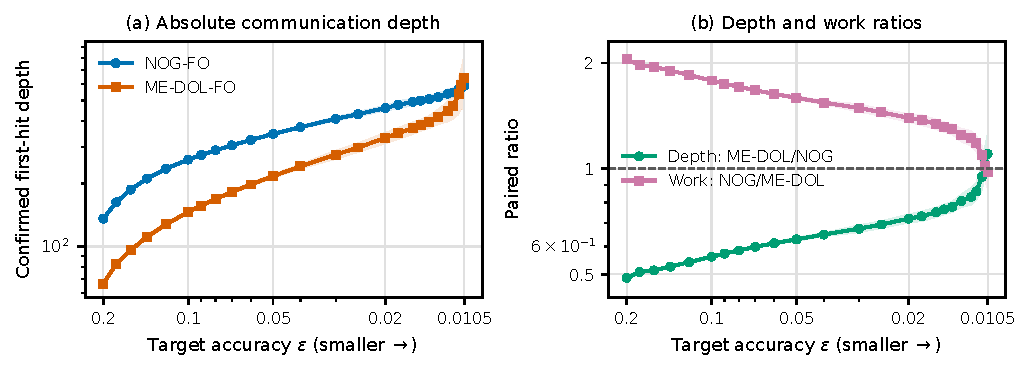
\includegraphics[width=\textwidth]{figures/fo_v4_fixed_batch.pdf}
		\caption{First-order comparison in the fixed-batch regime. Curves are
		means over 20 formal seeds; every method--threshold pair has 20/20 confirmed
		hits. \textbf{Left:} absolute first-hit depth, with bands showing one
		standard deviation. \textbf{Right:} per-seed paired ratios, with 95\%
		bootstrap confidence bands. Smaller $\epsilon$ is shown toward the right.}
		\label{fig:fo-v4-fixed-batch}
	\end{figure}

	As the target becomes more stringent, the paired depth ratio
	$D_{\mathrm{ME\text{-}DOL}}/D_{\mathrm{NOG}}$ increases monotonically from
	$0.488$ to $1.102$ (Spearman $\rho=1$ on the 25-point grid), crossing one near
	$\epsilon=0.01075$. Meanwhile, the paired work ratio
	$W_{\mathrm{NOG}}/W_{\mathrm{ME\text{-}DOL}}$ remains within an order-one
	range, $[0.980,2.049]$. Thus this finite-instance result exhibits a growing
	relative depth advantage as accuracy increases without an order-of-magnitude
	work separation. This qualitative trend is consistent with
	Theorem~\ref{thm:parallel-FO}, which improves NOG's worst-case depth dependence
	from $\widetilde O(\epsilon^{-3})$ to
	$\widetilde O(d^{1/3}\epsilon^{-5/3})$ while retaining
	$\widetilde O(\epsilon^{-3})$ work. We do not interpret the experiment as
	verification of the exact worst-case exponents: the objective and accuracy
	range are finite, the configurations are pilot-calibrated rather than
	globally optimal, and the stationarity measure is a Monte Carlo proxy.

\begin{figure}[t]
\centering
		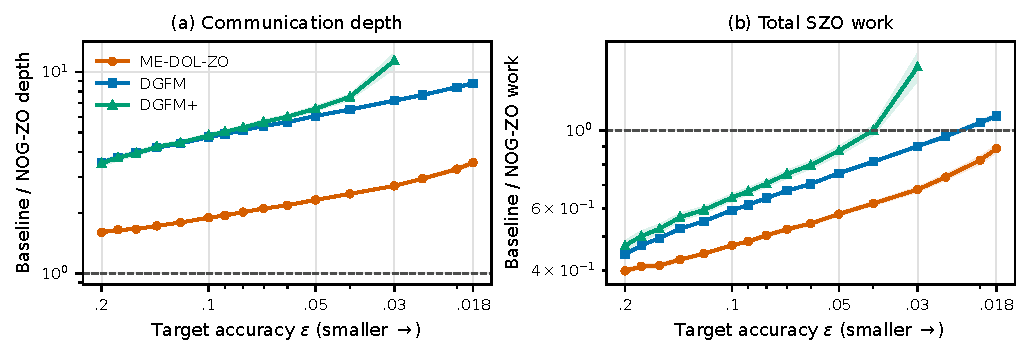
\includegraphics[width=0.96\textwidth]{figures/zo_depth_work_ratios.pdf}
		\caption{Zeroth-order paired ratios (baseline/NOG-ZO) over 20 frozen
		formal seeds; bands are 95\% paired-bootstrap confidence intervals.
		Only thresholds with 20/20 paired hits are plotted.  Smaller $\epsilon$
		is shown toward the right.}
		\label{fig:zo-main}
	\end{figure}
	\subsection{Zeroth-order communication--work scaling}
\label{sec:experiments-zo}
We next compare NOG-ZO against ME-DOL-ZO \citep{sahinoglu2024online}, DGFM,
and DGFM+ \citep{lin2024decentralized} on the same synthetic objective.  The
four methods use two-point estimators, eight workers, and an equal cap of
$983{,}040$ training function evaluations.  Configurations are selected on
pilot seeds $100$--$104$, frozen, and then evaluated on formal seeds $0$--$19$.
We form ratios within each seed and report trends only on thresholds at which
all 20 method/NOG-ZO pairs attain confirmed hits.  Figure~\ref{fig:zo-main}
shows these prespecified complete-pair regions; Appendix~\ref{app:zo-experiments}
gives all absolute results, non-hits, parameter settings, and audits.


	As $\epsilon$ decreases from $0.2$ to $0.018$, the depth ratios of
	ME-DOL-ZO and DGFM increase from $1.596$ to $3.547$ and from $3.556$ to
	$8.791$, respectively.  DGFM+/NOG-ZO increases from $3.520$ to $11.387$
	over its complete interval $[0.03,0.2]$.  All three depth curves are monotone
	(Spearman $\rho=1$), qualitatively supporting the improved
	$\epsilon$-dependence in Theorem~\ref{thm:dist-ZO}.  The corresponding work
	ratios change from $0.399$ to $0.887$, $0.444$ to $1.099$, and $0.471$ to
	$1.514$.  Thus the finite experiment does not recover the constant-order
	work dependence suggested for ME-DOL-ZO and DGFM+, and we treat work as
	a secondary descriptive endpoint.  More generally, the observed finite-range
	slopes need not equal worst-case exponents.  Our empirical claim is restricted
	to the prespecified communication-depth direction, not exact-rate verification
	or universal dominance.

\section{Conclusions and Future Works}
	
	In this work, we propose the Nonconvex Optimistic Gradient (NOG) method as a meta-algorithm for highly-parallel nonsmooth nonconvex optimization. Building upon the NOG framework, we further develop communication-efficient distributed algorithms and fast quantum algorithms.
	
	For future research, it would be of great interest to establish lower bounds for these settings. Such results would be instrumental in examining the tightness of our proposed methods. Moreover, our distributed algorithm requires a centralized server, and it is also important to consider its decentralized extensions \citep{lin2024decentralized,sahinoglu2024online,chen2026decentralized}. Finally, noting that the $\delta$ and $\epsilon$ dependencies of our zeroth- and first-order quantum algorithms and the one in \citep{liu2024quantum} are all $\delta^{-1} \epsilon^{-7/3}$, we wonder whether there exist faster algorithms that can break this barrier.

\subsection*{AI Use Statement}
% TODO: Replace this placeholder with the disclosure required by the ICLR 2027 AI Policy.
To be completed before submission.

\bibliography{nog_iclr2027}
\bibliographystyle{iclr2027_conference}

\appendix


% \section{Relationship of Assumption \ref{asm:ZO} and \ref{asm:FO}}

% Below, we prove that under regular conditions on $f(\,\cdot\,)$ and $F(\,\cdot\,;\xi)$, we can get Assumption \ref{asm:FO} from Assumption \ref{asm:ZO}. 

% \begin{lem} \label{lem:cor-main-assmp}
	% Under Assumption \ref{asm:ZO}, if both $f(\,\cdot\,)$ and $F(\,\cdot\,;\xi)$ are differentiable everywhere, we have
	% \begin{enumerate}
		%     \item[(a)] $f(\,\cdot\,)$ is $L$-Lipschitz continuous. 
		%     \item[(b)]  $ \E_{\xi \sim \Xi}[\nabla F(\vx;\xi)] = \nabla f(\vx)$ and $\E_{\xi \sim \Xi} \Vert \nabla F(\vx;\xi) \Vert^2 \le L^2$.
		% % Assumption \ref{asm:ZO} implies Assumption \ref{asm:FO}  with $\vg(\vx;\xi) = \nabla F(\vx; \xi)$ and  $G=L$.
		% % % Under Assumption \ref{asm:main}, we have
		% \end{enumerate}
	% \end{lem}

% \begin{proof}
	% Below, we derive (a) and (b) from Assumption \ref{asm:ZO} separately. 
	% \begin{enumerate}
		%     \item[(a)] By Assumption \ref{asm:ZO}(a) and Jensen's inequality, for any $\vx, \vx' \in \sR^d$ we have that 
		%     \begin{align*}
			%         \vert f(\vx) - f(\vx') \vert \le \E_{\xi \sim \Xi} \vert f(\vx) - f(\vx') \vert \le \E_{\xi \sim \Xi}[L(\xi)] \Vert \vx - \vx' \Vert \le L \Vert \vx - \vx' \Vert. 
			%     \end{align*}
		%     \item[(b)] At any point $\vx \in \sR^d$ such that $\nabla f(\vx)$ and $\nabla F(\vx ;\xi)$ both exist, we have that
		%     \begin{align} \label{eq:lim-grad}
			%         \lim_{\vh \rightarrow \vzero} \frac{f(\vx+\vh) - f(\vx) - \E_{\xi \sim \Xi }\langle \nabla F(\vx;\xi), \vh \rangle  }{\Vert \vh \Vert} &= \lim_{\vh \rightarrow \vzero} \E_{\xi \sim \Xi } \left[ \frac{F(\vx+\vh; \xi) - F(\vx; \xi) - \langle \nabla F(\vx;\xi), \vh \rangle  }{\Vert \vh \Vert} \right].
			%     \end{align}
		%     The differentiability of $\nabla F(\,\cdot\,;\xi)$ at point $\vx $ implies that 
		%     \begin{align*}
			%         \lim_{\vh \rightarrow \vzero} \frac{F(\vx+\vh; \xi) - F(\vx; \xi) - \langle \nabla F(\vx;\xi), \vh \rangle  }{\Vert \vh \Vert}  = \vzero,
			%     \end{align*}
		%     while Assumption \ref{asm:ZO}(b) implies that 
		%     \begin{align*}
			%         \frac{\vert F(\vx+\vh; \xi) - F(\vx; \xi)\vert }{\Vert \vh \Vert} \le L(\xi), \quad {\rm and} \quad \frac{\vert \langle \nabla F(\vx;\xi), \vh \rangle \vert }{\Vert \vh \Vert}  \le L(\xi). 
			%     \end{align*}
		%     Since $\E[L(\xi)] \le L $, we can apply Lebesgue's dominated convergence theorem on (\ref{eq:lim-grad}) to obtain that 
		%     \begin{align*}
			%          \lim_{\vh \rightarrow \vzero} \frac{f(\vx+\vh) - f(\vx) - \E_{\xi \sim \Xi }\langle \nabla F(\vx;\xi), \vh \rangle  }{\Vert \vh \Vert}  = \vzero.
			%     \end{align*}
		%     This completes the proof of $ \E_{\xi \sim \Xi}[\nabla F(\vx;\xi)] = \nabla f(\vx)$. Finally, we calculate the second-order moment bound by
		%     \begin{align*}
			%         \E_{\xi \sim \Xi} \Vert \nabla F(\vx;\xi) \Vert^2 \le   \E_{\xi \sim \Xi} [L(\xi)]^2 \le L^2.
			%     \end{align*}
		% \end{enumerate}
	% \end{proof}

% \begin{rmk}
	% The condition that both $f(\,\cdot\,)$ and $F(\,\cdot\,;\xi)$ are differentiable everywhere in Lemma \ref{lem:cor-main-assmp} is mild and without loss of generality because the Rademacher’s theorem indicates that any Lipschitz continuous function is differentiable almost everywhere, and therefore such conditions can be fulfilled with probability 1 by adding arbitrarily small random permutations on the original functions. It is a standard technique used in previous works, which can refer to \textit{e.g.}  \citep[Proposition 2]{cutkosky2023optimal}, \citep[Lemma 2.3]{davis2022gradient}, or \citep[Lemma 3.2]{tian2022finite}.
	% \end{rmk}

\section{Proof of Randomized Smoothing}

\propfdeltasmooth*

\begin{proof}
	We verify each items one by one as follows.
	\begin{enumerate}
		\item[(a)] It follows the definition of $f_{\delta}$ (Definition \ref{dfn:f-delta}) and Jensen's inequality that 
		\begin{align*}
			\vert f_{\delta}(\vx) - f(\vx) \vert \le \E_{\vu \sim {\rm Unif}(\sB^d)} \vert f(\vx + \delta \vu) -f(\vx) \vert \le L \delta \E_{\vu \sim {\rm Unif}(\sB^d)} \Vert \vu \Vert \le L \delta.
		\end{align*}
		\item[(b)] By the definition of $f_{\delta}$ (Definition \ref{dfn:f-delta}), the Lipschitz continuity of $f$ and Jensen's inequality, for any $\vx, \vx' \in \sR^d$ we have that 
		\begin{align*}
			\vert f_{\delta}(\vx) - f_{\delta}(\vx') \vert &= \vert  \E_{\vu \sim {\rm Unif}(\sB^d)} [f(\vx+ \delta \vu)] -  \E_{\vu' \sim {\rm Unif}(\sB^d)} [f(\vx'+ \delta \vu')] \vert \\
			&= \vert  \E_{\vu \sim {\rm Unif}(\sB^d)} [f(\vx+ \delta \vu)] -  \E_{\vu \sim {\rm Unif}(\sB^d)} [f(\vx' + \delta \vu)] \vert \\
			&\le \E_{\vu \sim {\rm Unif}(\sB^d)} \vert f(\vx+ \delta \vu) - f(\vx' + \delta \vu) \vert \le L \Vert \vx - \vx' \Vert.
		\end{align*}
		\item[(c)] See \citep[Lemma 4]{kornowski2024algorithm} for a proof. 
		\item[(d)] It is first proven in \cite{yousefian2012stochastic}. See also \citep[Proposition 2.2]{lin2022gradient} for a more complete proof. 
	\end{enumerate}
\end{proof}

\section{Proof of the Nonconvex Optimistic Gradient Method}

% \lemsmoothonc*

% \begin{proof}
	% We start from the fundamental theorem of calculus that
	% \begin{align*}
		%     f(\vx_{t}) - f(\vx_{t-1}) =& \left \langle \int_0^1 \nabla f(\vx_{t-1}) + s \vDelta_t) {\rm d} s, \vDelta_t \right \rangle \\
		%     =& \langle \nabla f(\vy_t), \vDelta_t \rangle +  \left \langle \int_0^1 (\nabla f(\vx_{t-1}) + s \vDelta_t) - \nabla f(\vy_t) ) {\rm d} s, \vDelta_t \right \rangle
		% \end{align*}
	% For the right-hand side, we further apply
	% (1) Cauchy-Schwarz inequality, (2) $H$-smoothness of the function~$f$, (3) the identity $\vy_t = \vx_{t-1} + \vDelta_t/2$, and (4) $\Vert \Delta_t \Vert \le D$, which gives
	% \begin{align*}
		%     f(\vx_{t}) - f(\vx_{t-1}) \le& \langle \nabla f(\vy_t), \vDelta_t \rangle +  \int_0^1 \Vert\nabla f(\vx_{t-1}) + s \vDelta_t) - \nabla f(\vy_t) \Vert \Vert \vDelta_t \Vert {\rm d} s \\
		%     \le& \langle \nabla f(\vy_t), \vDelta_t \rangle +  H \int_0^1 \Vert\vx_{t-1} + s \vDelta_t-\vy_t \Vert \Vert \Vert \vDelta_t \Vert {\rm d} s  \\
		%     =& \langle \nabla f(\vy_t), \vDelta_t \rangle + H\int_0^1 \left \vert s- \frac{1}{2} \right \vert \Vert \vDelta_t \Vert^2 {\rm d} s = \langle \nabla f(\vy_t), \vDelta_t \rangle + \frac{H D^2}{4}. 
		% \end{align*}
	% Note that conditioned on $\Delta_t$, we have $\E [\mO_f(\vy_t)] =\nabla f(\vy_t)$. Therefore, we can take the expectation on both sides and then replace $\nabla f(\vy_t)$ with $\mO_f(\vy_t)$ on the right-hand side, which gives
	% \begin{align*}
		%     \E[f(\vx_{t}) - f(\vx_{t-1})] 
		%     \le& \E \langle \mO_f(\vy_t), \vDelta_t \rangle + \frac{H D^2}{4}. 
		% \end{align*}
	% Telescoping this inequality for $t = (k-1)M+1,\cdots,kM$ and rearranging the right-hand side, we obtain
	% \begin{align*}
		%     \E[f(\vx_{kM}) - f(\vx_{(k-1)M})] \le& \sum_{t=(k-1)M+1}^{k(k+1)M}  \E \langle \mO_f(\vy_t), \Delta_t - \vu_k \rangle + \sum_{t=(k-1)M+1}^{k(k+1)M}  \E \langle \mO_f(\vy_t), \vu_k \rangle + \frac{M H D^2}{4}.
		% \end{align*}
	% Letting $\vu_k = - D \sum_{t=(k-1)M+1}^{(k+1)M} \mO_f(\vy_t) / \Vert \sum_{t=(k-1)M+1}^{(k+1)M} \mO_f(\vy_t) \Vert $ in the above, we have
	% \begin{align*}
		%     \E[f(\vx_{kM}) - f(\vx_{(k-1)M})] \le& \sum_{t=(k-1)M+1}^{(k+1)M} \E \langle \mO_f(\vy_t), \Delta_t - \vu_k \rangle  - D \E \left \Vert \sum_{t=(k-1)M+1}^{(k+1)M} \mO_f(\vy_t) \right \Vert + \frac{M HD^2}{4}.
		% \end{align*}
	% Next, using the definition of $\sigma$-SFO that $\E \mO_f(\vy_t) = \nabla f(\vy_t)$ and $\E \Vert \mO_f(\vy_t) -\nabla f(\vy_t) \Vert^2 \le \sigma^2$, we know that $\E \left \Vert \sum_{t=(k-1)M+1}^{k(k+1)M} \mO_f(\vy_t) - \nabla f(\vy_t) \right \Vert \le \sqrt{M} \sigma$. Hence, using the triangle inequality, we can further obtain that
	% \begin{align*}
		%      \E[f(\vx_{kM}) - f(\vx_{(k-1)M})] \le& \sum_{t=(k-1)M+1}^{(k+1)M}  \E \langle \mO_f(\vy_t), \Delta_t - \vu_k \rangle  - D \E \left \Vert \sum_{t=(k-1)M+1}^{(k+1)M} \nabla f(\vy_t) \right \Vert + D\sqrt{M} \sigma+ \frac{MHD^2}{4}.
		% \end{align*}
	% Finally, summing up this inequality for $k = 1,\cdots,K$, dividing both sides by $KDM$, and rearranging gives
	% \begin{align*}
		%    \frac{1}{K} \E \left \Vert \frac{1}{M} \sum_{t=(k-1)M+1}^{(k+1)M} \nabla f(\vy_t) \right \Vert \le \frac{f(\vx_0) - f(\vx_{K})}{KDM} + \frac{{\rm Reg}_{T,K}}{KDM} + \frac{\sigma}{\sqrt{M}} + \frac{HD}{4}.
		% \end{align*}
	% \end{proof}

% \lemsmoothreg*

% \begin{proof}
	% Recall Lemma \ref{lem:odog} tells that
	% \begin{align} \label{eq:regret-odog-lem}
		% \begin{split}
			%     \sum_{t= (k-1)M +1}^{k M} \E \langle \mO_f(\vy_t), \vDelta_t - \vu_k \rangle \le& \frac{4 D^2}{\eta} + \frac{3\eta}{2}\E \Vert \mO_f(\vy_{(k-1)M}) - \mO_f(\vz_{(k-1)M}) \Vert^2 \\
			%     + & \sum_{t= (k-1)M +1}^{k M} \E \left[\eta \Vert \mO_f(\vy_t) - \mO_f(\vz_t) \Vert^2 - \frac{1}{4 \eta} \Vert \vDelta_t - \vDelta_{t-1} \Vert^2\right]. 
			% \end{split}
		% \end{align}
	% We know from  (1) Young's inequality, (2) the definition of $\sigma$-SFO, (3) and $H$-smoothness of $f$, and (4) the identity $\vy_t - \vz_t = (\vDelta_t - \vDelta_{t-1})/2$ that
	% \begin{align*}
		%     \Vert \mO_f(\vy_t) - \mO_f(\vz_t) \Vert^2 \le&
		% 3 \Vert \mO_f(\vy_t) - \nabla f(\vy_t) \Vert^2 + 3 \Vert \mO_f(\vz_t) - \nabla f(\vz_t) \Vert^2 + 3 \Vert \nabla f(\vy_t) - \nabla f(\vz_t) \Vert^3 \\
		% \le& 6 \sigma^2 + 3H^2 \Vert \vy_t - \vz_t \Vert^2 = 6 \sigma^2 + \frac{3H^2}{4} \Vert \vDelta_t - \vDelta_{t-1} \Vert^2,
		% \end{align*}
	% which is an analog to \citep[Lemma B.3]{patitucci2025improving}. And the remaining proofs are also similar to those in \citep{patitucci2025improving}. Substituting into the regret bound in inequality (\ref{eq:regret-odog-lem}), rearranging, and using the fact $\Vert \vDelta_t \Vert \le D$, we have 
	% \begin{align*}
		%   \sum_{t= (k-1)M +1}^{k M} \E \langle \mO_f(\vy_t), \vDelta_t - \vu_k \rangle \le& \frac{4 D^2}{\eta} + \frac{9\eta H^2 D^2}{2} + 9 M \eta \sigma^2 - \left( \frac{1}{4 \eta} - \frac{3 H^2}{4} \right)  \sum_{t= (k-1)M +1}^{k M} \E \Vert \vDelta_t - \vDelta_{t-1} \Vert^2.   
		%   % \\
		%   %   &\E [{\rm Reg}_{T,K}] \le \frac{4 KD^2}{\eta} +
		%   %   15 \eta KM \sigma^2 + \frac{15 \eta H^2 D^2}{8}  -
		%   %   \left( \frac{1}{4 \eta} -\frac{15 \eta H^2 }{8}   \right)\sum_{t=2}^{KM} \E  
		% \end{align*}
	% Note that by setting $\eta \le \frac{1}{\sqrt{3} H}$,  we can guarantee that $\frac{1}{4 \eta} -\frac{3 \eta H^2}{4} \ge 0$ and drop the last term in the above. Then, we obtain 
	% \begin{align*}
		%     \sum_{t= (k-1)M +1}^{k M} \E \langle \mO_f(\vy_t), \vDelta_t - \vu_k \rangle \le& \frac{4 D^2}{\eta} +\frac{9\eta H^2 D^2}{2} + 9 M \eta \sigma^2.   
		% \end{align*}
	% Next, by selecting the stepsize as $\eta = \min \left\{ \frac{1}{2H}, \frac{2D}{3 \sigma \sqrt{M}} \right\}$ and using the basic inequality $\frac{1}{\min\{a,b \}} \le a+b$, we can further bounded the right-hand side above as
	% \begin{align*}
		%  \sum_{t= (k-1)M +1}^{k M} \E \langle \mO_f(\vy_t), \vDelta_t - \vu_k \rangle \le 18 H D^2 + 12 \sigma \sqrt{M} D.
		% \end{align*}
	% Summing up this inequality for all $k = 1,\cdots,K$, we know that the $K$-shifting regret can be bounded by $K$ times of its right-hand side, which gives
	% \begin{align*}
		%     \E [{\rm Reg}_{T,K} ] \le 6K \left( 3 H D^2 +2 \sigma \sqrt{M} D^2 \right).
		% \end{align*}
	% \end{proof}
% \thmodogs*

% \begin{proof}
	% Plug the regret bound of Lemma \ref{lem:reg-smooth-surrogate} into Lemma \ref{lem:smooth-o2nc}, we get
	% \begin{align*}
		%     \E \Vert \nabla f(\bar \vy_{\rm out}) \Vert \le 
		%     \frac{F_0}{KDM} +
		%     \frac{18 H D}{M} + \frac{13 \sigma}{\sqrt{M}} + \frac{HD}{4}.
		% \end{align*}
	% For $D = \delta/M$, $T = KM$ and $H= c \sqrt{d} L / \delta$, we have that
	% \begin{align*}
		%      \E \Vert \nabla f(\bar \vy_{\rm out}) \Vert \le 
		%     \frac{M F_0}{\delta T} +
		%     \frac{73c \sqrt{d} L}{4 M} + \frac{13 \sigma}{\sqrt{M}}.
		% \end{align*}
	% By selecting $M = \max \left\{ \left( \frac{73 c \sqrt{d} L \delta T}{4 F_0} \right)^{1/2}, \left( \frac{13 \sigma \delta T}{F_0} \right)^{2/3} \right\}$ and using the basic inequality $\max\{a,b \} \le a+b$, we can further bounded the right-hand side above as
	% \begin{align*}
		%      \E \Vert \nabla f(\bar \vy_{\rm out}) \Vert \le \left( 
		%      \frac{73 c\sqrt{d} L F_0}{\delta T}
		%      \right)^{1/2} + \frac{2 F_0^{1/3}\left(13 \sigma \right)^{2/3}}{\left(\delta T \right)^{1/3}}.
		% \end{align*}
	% Therefore, to find a $(\delta,\epsilon)$-Goldstein stationary point, the number of oracles $\sO_{f_\delta}$ required by the algorithm is no more than
	% \begin{align*}
		%     T = \gO \left( \frac{\sqrt{d} L F_0}{\delta \epsilon^2} + \frac{\sigma^2 F_0}{\delta \epsilon^{3}} \right).
		% \end{align*}
	% \end{proof}
\lemregretong*

\begin{proof}
	We start from Lemma \ref{lem:odog} that
	\begin{align*}
		\E [{\rm Reg}_{T,K}] \le \frac{4 K D^2}{\eta} + \frac{5 \eta}{2} \sum_{t=1}^{KM} \E \Vert \mO(\vy_t) - \mO(\vy_{t-1}) \Vert^2.
	\end{align*}
	Applying Young's inequality on the second term, we further obtain that
	\begin{align*}
		\E [{\rm Reg}_{T,K}] \le& \frac{4 K D^2}{\eta} + \frac{15 \eta}{2} \sum_{t=1}^{KM} \E [\Vert \nabla f_\delta(\vy_t) - \nabla f_\delta(\vy_{t-1}) \Vert^2 \\
		+ &\Vert \mO(\vy_t) - \nabla f_\delta(\vy_t) \Vert^2 + \Vert \mO(\vy_{t-1}) - \nabla f_\delta(\vy_{t-1}) \Vert^2].
	\end{align*}
	By Proposition \ref{prop:f-delta-smooth}(d) we have $\Vert \nabla f_\delta(\vy_t) - \nabla f_\delta(\vy_{t-1}) \Vert \le (c \sqrt{d} L /\delta) \Vert \vy_t - \vy_{t-1} \Vert$, and by the definition of $(\delta,\sigma)$ oracle (Definition \ref{dfn:delta-SFO}) we have $\E \Vert \mO(\vy) - \nabla f_\delta(\vy) \Vert^2 \le \sigma^2 $. Therefore, we get
	\begin{align*}
		\E [{\rm Reg}_{T,K}] \le \frac{4 K D^2}{\eta} + \frac{15 \eta c^2 d L^2 }{2\delta^2}  \sum_{t=1}^{KM} \E \Vert \vy_t - \vy_{t-1} \Vert^2  + 15 \eta KM \sigma^2.
	\end{align*}
	In Algorithm \ref{alg:O2NC}, we have $\vy_t - \vy_{t-1} = (\vx_{t-1} + s_t \vDelta_t) - (\vx_{x-2} + s_{t-1} \vDelta_{t-1}) = (1- s_{t-1}) \vDelta_{t-1} + s_t \vDelta_t \in \sB_{3D}^d(\vzero) $. Therefore, we can further bound the right-hand side in the above inequality as
	\begin{align*}
		\E[{\rm Reg}_{T,K}] \le \frac{4 K D^2}{\eta} + 15 \eta KM \left( \frac{9 c^2 d L^2 D^2}{2 \delta^2} + \sigma^2 \right).
	\end{align*}
\end{proof}

\thmong*
\begin{proof}
	Selecting the stepsize $\eta = \Theta \left( \frac{\delta}{L\sqrt{d M}} \land \frac{D}{\sigma \sqrt{M}}  \right)$ to minimize the regret in Lemma \ref{lem:regret-o2ng}, we obtain
	\begin{align*}
		\E[{\rm Reg}_{T,K}] = \gO \left( K \left( \frac{D^2 L \sqrt{dM}}{\delta} + D \sigma \sqrt{M}  \right)  \right).
	\end{align*}
	Substituting the above regret bound into Lemma \ref{lem:O2NC}, we have
	\begin{align*}
		\E\left[{\rm dist} \left(\partial_\delta f_{\delta}(\bar \vy_{\rm out}), \vzero \right) \right] = \gO \left( \frac{f_\delta(\vzero) - f_\delta^*}{K DM} + \frac{\sqrt{d} LD}{\sqrt{M}} + \frac{\sigma}{\sqrt{M}} \right).
	\end{align*}
	Note that by Assumption \ref{asm:Lip} we have $f(\vzero) - f^* \le \gamma$ and by Proposition \ref{prop:f-delta-smooth}(a) we have $\vert f_\delta(\,\cdot\,) - f(\,\cdot\,) \vert \le \delta L$. Therefore, we have $f_\delta(\vzero) - f_\delta^* \le \gamma + \delta L$ and
	\begin{align*}
		\E\left[{\rm dist} \left(\partial_\delta f_{\delta}(\bar \vy_{\rm out}), \vzero \right) \right] = \gO \left( \frac{\gamma + \delta L}{K DM} + \frac{\sqrt{d} LD}{\delta \sqrt{M}} + \frac{\sigma}{\sqrt{M}} \right).
	\end{align*}
	For $T = KM$ and $D = \delta/ M$, we have
	\begin{align*}
		\E\left[{\rm dist} \left(\partial_\delta f_{\delta}(\bar \vy_{\rm out}), \vzero \right) \right] = \gO \left( \frac{M(\gamma + \delta L)}{\delta T} + \frac{\sqrt{d} L}{M^{3/2}} + \frac{\sigma}{\sqrt{M}} \right).
	\end{align*}
	Selecting the parameter $M = \Theta \left( \left( 
	\frac{\sqrt{d} L \delta T}{\gamma + \delta L}
	\right)^{2/5} \lor \left( \frac{\sigma \delta T}{\gamma + \delta L} \right)^{2/3} \right)$ to minimize the right-hand side, we obtain
	\begin{align*}
		\E\left[{\rm dist} \left(\partial_\delta f_{\delta}(\bar \vy_{\rm out}), \vzero \right) \right]  = \gO \left(
		d^{1/5} L^{2/5} \left( \frac{\gamma + \delta L}{\delta T} \right)^{3/5} + \sigma^{2/3} \left( \frac{\gamma + \delta L}{\delta T} \right)^{1/3}
		\right).
	\end{align*}
	Recalling Proposition that \ref{prop:f-delta-smooth}(d) $\partial_{\delta} f_{\delta}(\,\cdot\,) \in \partial_{2 \delta} f(\,\cdot\,)$, we know that the algorithm can provably find a $(2\delta,\epsilon)$-Goldstein stationary point in total iterations no more than 
	\begin{align*}
		T = \gO \left( \frac{\gamma + \delta L}{\delta}  \left( \frac{ d^{1/3} L^{2/3}}{\epsilon^{5/3}} + \frac{\sigma^2}{\epsilon^3} \right) \right).
	\end{align*}
\end{proof}
% \lemregret*
% \begin{proof}
	% Note that Line \ref{line:O2NC-extra} and \ref{line:O2NC-OGD} in Algorithm \ref{alg:fast-O2NC} are exactly the update of optimistic online gradient descent \citep{hazan2010extracting,rakhlin2013online} or extragradient \cite{korpelevich1976extragradient} on the domain $\sB(\vzero, D)$. Following the standard analysis for this update, (see \textit{e.g.} \citep[Lemma 15]{chen2021impossible}, for any $\vu \in \sB(\vzero, D)$, we have 
	% \begin{align*}
		%     \langle \vg_t , \vDelta_{t} - \vu \rangle &\le  \langle \vg_{t} - \vh_{t}, \vDelta_{t}  - \vv_t \rangle + \frac{1}{2 \eta} \Vert \vu - \vv_t \Vert^2 \\
		%     &- \frac{1}{2 \eta} \Vert \vu - \vv_{t+1} \Vert^2 - \frac{1}{2 \eta } \Vert \vv_{t+1} - \vDelta_{t}  \Vert^2 - \frac{1}{2 \eta} \Vert \vDelta_{t}  - \vv_t \Vert^2.
		% \end{align*}
	% We can use Young's inequality to get
	% \begin{align*}
		%     \langle \vg_t , \vDelta_{t}  - \vu \rangle &\le  \frac{\eta}{2} \Vert \vg_t - \vh_{t} \Vert^2 + \frac{1}{2 \eta} \Vert \vu - \vv_t \Vert^2 - \frac{1}{2 \eta} \Vert \vu - \vv_{t+1} \Vert^2 
		% \end{align*}
	% {\color{red} Use ODOG analysis to provide a tighter regret bound.}
	
	
	% Telescoping yields that
	% \begin{align*}
		%     R_M(\vu_1,\cdots,\vu_K) &= \sum_{k=1}^K \sum_{m= (k-1)M +1}^{k M} \langle \vg_m, \vv_{m+1/2} - \vu_k \rangle \\
		%     &\le \frac{\eta}{2} \sum_{k=1}^K \sum_{m = (k-1)M +1}^{kM} \Vert \vg_m - \vg_{m-1} \Vert^2 + \frac{1}{2 \eta} \sum_{k=1}^K  \Vert \vu_k  - \vv_{(k-1)M+1)} \Vert^2.  
		% \end{align*}
	% Taking expectation, and leveraging the variance bound in the $(\delta,\sigma)$ SFO (Definition \ref{dfn:SFO}), we have that
	% \begin{align*}
		%     \E[ R_M(\vu_1,\cdots,\vu_K) ] &\le \eta \sum_{k=1}^K \sum_{m = (k-1)M +1}^{kM} \E \Vert \nabla f_{\delta}(\vy_{m}) - \nabla f_{\delta}(\vy_{m-1}) \Vert^2  \\
		%     &\quad  +  4 \eta  KM \sigma^2 +  \frac{1}{2 \eta} \sum_{k=1}^K  \Vert \vu_k  - \vv_{(k-1)M+1)} \Vert^2, 
		% \end{align*}
	% where we define $\vy_0 = \vzero$ in the above.
	% Now, we use Proposition \ref{prop:f-delta-smooth}(b) that $f_{\delta}(\,\cdot\,)$ is $L$-Lipschitz and  Proposition \ref{prop:f-delta-smooth}(d) that $f_{\delta}(\,\cdot\,)$ is $(c \sqrt{d}  / \delta)$-smooth for some numerical constant $c>0$ to get
	% \begin{align} \label{eq:tele-regret}
		% \begin{split}
			% \E[ R_M(\vu_1,\cdots,\vu_K) ] &\le \frac{ c^2 \eta  d L^2}{\delta^2}  \sum_{k=1}^K \sum_{m = (k-1)M +1}^{kM} \Vert \vy_m - \vy_{m-1} \Vert^2   \\
			%         &\quad +  4 \eta  KM \sigma^2 +  \frac{1}{2 \eta} \sum_{k=1}^K  \Vert \vu_k  - \vv_{(k-1)M+1)} \Vert^2.
			% \end{split}
		% \end{align}
	% By the update of the algorithm and triangle inequality, we can obtain that
	% \begin{align*}
		%     \Vert \vy_t - \vy_{t-1} \Vert \le \Vert \vy_t - \vx_{t-1} \Vert + \Vert \vx_t - \vx_{t-1} \Vert + \Vert \vy_{t-1} - \vx_{t-1} \Vert \le 3D.
		% \end{align*}
	% In addition, we also have
	% \begin{align*}
		%     \Vert \vu_k  - \vv_{(k-1)M+1)} \Vert \le \Vert \vu_k \Vert + \Vert \vv_{(k-1)M+1)} \Vert \le 2D.
		% \end{align*}
	% Using these two bounds in (\ref{eq:tele-regret}), we then get
	% \begin{align*}
		%     \E[ R_M(\vu_1,\cdots,\vu_K) ] &\le \frac{9 c^2 \eta d L^2 K M  D^2}{\delta^2}  +  4 \eta  KM \sigma^2 + \frac{2K D^2}{\eta}. 
		% \end{align*}
	% \end{proof}

% \thmupper*
% \begin{proof}
	
	
	% Setting 
	% \begin{align} \label{eq:setting-eta}
		%     \eta = \sqrt{\frac{2 K D^2}{ 9 c^2 d L^2 KM D^2/ \delta^2  + 4 K M \sigma^2 }}
		% \end{align}
	% yields that
	% \begin{align*}
		%     \E[ R_M(\vu_1,\cdots,\vu_K) ] &\le \sqrt{2 K } D \cdot \sqrt{9 c^2 d L^2 KM D^2/ \delta^2  + 4 K M \sigma^2 } \\
		%     &\le 3 c \sqrt{2d M} L D^2 K / \delta + 2\sqrt{2 M } DK \sigma.
		% \end{align*}
	% We now substitute the above regret bound into (\ref{eq:regre-O2NC}) to get
	% \begin{align*}
		%      &\quad \frac{1}{K} \sum_{k=1}^{K-1} \E \left \Vert \frac{1}{M} \sum_{m=1}^M \nabla f_{\delta}( \vy_{(k-1)M+m} ) \right \Vert \\
		%      &\le \frac{f_{\delta}(\vx_0) - f_{\delta}^*}{ D T} + \frac{3 c \sqrt{2d M} L D K}{\delta T}  + \frac{2\sqrt{2 M } K \sigma}{T} + \frac{\sigma}{\sqrt{M}}.
		% \end{align*}
	% Next, we substitute $D =\delta / M$ and $T = KM$ to get
	% \begin{align*}
		%     &\quad \frac{1}{K} \sum_{k=1}^{K-1} \E \left \Vert \frac{1}{M} \sum_{m=1}^M \nabla f_{\delta}( \vy_{(k-1)M+m} ) \right \Vert \\
		%     &\le \frac{M (f_{\delta}(\vx_0) - f_{\delta}^*)}{\delta T} + \frac{3 c \sqrt{2 d} L }{M^{\frac{3}{2}}} + \frac{(2 \sqrt{2} + 1) \sigma}{\sqrt{M}}.
		% \end{align*}
	% Furthermore, by Proposition \ref{prop:f-delta-smooth} we know $\vert f_{\delta}(\,\cdot\,) - f(\,\cdot\,) \vert \le \delta L$, and hence $f_{\delta}(\vx_0) - f_{\delta}^* \le \gamma + \delta L$ in the above.
	% From Proposition \ref{prop:Q-FO-estimator} we know a first-order quantum algorithm with $\tilde \gO(B)$ QSFO complexity can ensure $\sigma \le \sqrt{d} L / B)$, and from Proposition \ref{prop:Q-ZO-estimator} we know a zeroth-order quantum algorithm with $\tilde \gO(B)$ QSZO complexity can ensure $\sigma \le d L / B$. 
	% Here, we can view $B$ as a virtual batch size. To show the upper bound for both first-order and zeroth-order in a unified way, we define $\sigma = d^{\alpha} L / B$, where $\alpha = 1/2$ for first-order method and $\alpha = 1$ for zeroth-order method. 
	% We define
	% the total complexity of the algorithm (zeroth-order or first-order) by $N = T B$. 
	% Therefore, the above inequality can also be written as
	% \begin{align*}
		%     &\quad \frac{1}{K} \sum_{k=1}^{K-1} \E \left \Vert \frac{1}{M} \sum_{m=1}^M \nabla f_{\delta}( \vy_{(k-1)M+m} ) \right \Vert \\
		%     &\le \frac{B M (\gamma + \delta L)}{\delta N} + \frac{3 c \sqrt{2 d} L }{M^{\frac{3}{2}}} + \frac{(2 \sqrt{2} + 1) d^{\alpha} L}{\sqrt{M} B }.
		% \end{align*}
	% From the above inequality, we can see the optimal choice of $B$ is 
	% \begin{align} \label{eq:setting-B}
		%     B = \frac{ (2 \sqrt{2} + 1)^{\frac{1}{2}} d^{\frac{\alpha}{2}} L^{\frac{1}{2}} (\delta N)^{\frac{1}{2}} }{ M^{\frac{3}{4} } (\gamma + \delta L)^{\frac{1}{2}}}.
		% \end{align}
	% The above setting yields that
	% \begin{align*}
		%      &\quad \frac{1}{K} \sum_{k=1}^{K-1} \E \left \Vert \frac{1}{M} \sum_{m=1}^M \nabla f_{\delta}( \vy_{(k-1)M+m} ) \right \Vert \\ 
		%      &\le \frac{ (2 \sqrt{2} + 1)^{\frac{1}{2}} M^{\frac{1}{4}} (\gamma +\delta L)^{\frac{1}{2}} d^{\frac{\alpha}{2}} L^{\frac{1}{2}}}{ (\delta N)^{\frac{1}{2}} } + \frac{3 c \sqrt{2 d} L }{M^{\frac{3}{2}}}.
		% \end{align*}
	% From the above, we can see the optimal choice of parameter $M$ is
	% \begin{align}  \label{eq:setting-M}
		%     M = \left( \frac{3 c \sqrt{2 d} L (\delta N)^{\frac{1}{2}}}{ (2 \sqrt{2} + 1)^{\frac{1}{2}} M^{\frac{1}{4}} (\gamma +\delta L)^{\frac{1}{2}} d^{\frac{\alpha}{2}} L^{\frac{1}{2}} }  \right)^{\frac{4}{7}},
		% \end{align}
	% which will lead to the final upper bound of
	% \begin{align*}
		%      &\quad \frac{1}{K} \sum_{k=1}^{K-1} \E \left \Vert \frac{1}{M} \sum_{m=1}^M \nabla f_{\delta}( \vy_{(k-1)M+m} ) \right \Vert \\  
		%      &\le  \left( \frac{ 3c \sqrt{2} (2 \sqrt{2} +1)^3 (\gamma+ \delta L)^3 d^{3 \alpha+\frac{1}{2}} L^4 }{ (\delta N)^3 } \right)^{\frac{1}{7}}.
		% \end{align*}
	% It means the algorithm will provably output a $(\delta,\epsilon)$-stationary point in the total complexity of  
	% \begin{align*}
		%     N = \gO\left(  \frac{d^{\alpha+ \frac{1}{6}} L^{\frac{4}{3}}(\gamma + \delta L)}{\delta \epsilon^{\frac{7}{3}}}  \right).
		% \end{align*}
	% \end{proof}
% \paragraph{Upper Bound of (a)} From the previous discussion, we know that the output of $\mA_K$ is independent of $\vu_T$ and (\ref{eq:bound-uT}) holds conditioned on $\mA_K$ under event $G$. Therefore, for any $\vx \sim p_{K \mid G}$, for $\vz = \rho_R(\vx)$ with $R = 2 \sqrt{T}$ we have that $\vert \langle \vu_T, \vz \rangle \vert < 1 /4$. Our next goal is to following similar analysis to \citep[Lemma 25]{cutkosky2023optimal} to show that this implies that $\vx$ can not lie in the sets of $(1/2)$-stationary points $S =  \{ \vx \in \sR^d : \Vert \nabla \hat f_{T;\mU}(\vx) \Vert \le 1/2 \}$. 
% We consider two cases, either $\Vert \vx \Vert > \sqrt{T}$ or not. 

% If $\Vert \vx \Vert > \sqrt{T}$, we have that
% \begin{align*}
	%     \Vert \nabla \hat f_{T; \mU} (\vx) \Vert &\ge \lambda \Vert \nabla q_R(\vx) \Vert - \Vert \mJ_{\rho_R} (\vx) \Vert \Vert \nabla \bar f_{T; \mU}(\vy) \Vert \\
	%     &\ge \lambda \Vert \nabla q_R(\vx) \Vert - \Vert \nabla \bar f(\vy) \Vert \\
	%     &\ge \frac{\lambda \Vert \vx \Vert}{\sqrt{1 + \Vert \vx \Vert^2/ R^2}} - L_0 \sqrt{T} \\
	%     &\ge 3 \lambda R - L_0 \sqrt{T} \ge .
	% \end{align*}








% Above, the first inequality comes from the triangle inequality; the second one uses that fact $\Vert \mJ_{\rho_R}(\vx) \Vert \le 1$ by (\ref{eq:Jacobian}); the third one uses Lemma \ref{lem:prop-q}(b) and Lemma \ref{lem:Carmon}(c); and the last line uses 
% the monotonicity of function $q_R(\,\cdot\,)$.
% \begin{align*}
	%      \vert \le \Vert \vu_T \Vert \Vert \vz \Vert \le \beta / 4. 
	% \end{align*}


% To further upper bound (\ref{eq:P-TV}), we need to bound $\BP( \vx \in S \mid \vx \sim p_{K \mid F}, F  )$. 
% It means that conditioned on both events $E$ and $F$, for any $\vx \sim p_{K \mid F}$, we have that
% \begin{align*}
	%     \vert 
	% \end{align*}
% Conditioned on event $E$, we have that $\vert \vu_T, \vx $

% the worst-case construction of QSFO in  is independent of $\mU_T$. Therefore, by choosing $\vu_T$ 


% % represent the states $\psi_K$ and $\psi_0$ conditioned on event $F$.

% % Then, by Markov's inequality, there exists an event $F$ with $\BP(F) \ge 2/3$ such that
% % \begin{align} \label{eq:norm-Ak-A0}
	% %     \Vert  \psi_{K \mid F}  - \psi_{0 \mid F} \Vert^2 \le \frac{1}{48 T^2},
	% % \end{align}

% % where we use 
% % Next, conditioned on event $F$,  we let $p_{0 \mid F} = \vert \psi_K \vert^2$ and $p_{K \mid F} = \vert \psi_0 \vert^2$










% to denote the  $\psi_{0 \mid F}$ and $\psi_{K \mid F}$. 


% Let $F$ be the event that the above happens, then we have $\BP(F) \ge 2/3$.

% Conditioned on event $F$, 
% where  Define $\psi_{K \mid F}(\vx)$ and $\psi_{0 \mid F}(\vx)$ the wave functions of these states, which satisfy that $\vert \psi_{0 \mid F} (\vx) \vert^2 = p_{0 \mid F}$ and   $\vert \psi_{K \mid F} (\vx) \vert^2 = p_{K \mid F}$.


% We define $\psi_{K \mid \mU, \zeta }$ and $\psi_{0 \mid \mU, \zeta }$ to 


% Define
% $p_{K}(\vx) $ and $p_0(\vx)$ as the probability distribution obtained by measuring the state $\psi_K $ and $\psi_0 $, respectively. Similarly, we can define the conditional distribution $p_{K; \mU, \zeta}$ and $p_{0; \mU, \zeta}$, and we have the relationship that $p_{K;\mU,\zeta}(\vx) = \vert \psi_{K;\mU,\zeta}(\vx) \vert^2$ and $p_{0;\mU,\zeta}(\vx) = \vert \psi_{0;\mU,\zeta}(\vx) \vert^2$.
%  , we have that


% \begin{align*}
	%     d_{\rm TV}(p_0,p_K) &= \frac{1}{2}\iiint  \vert p_0(\vx) - p_K(\vx) \vert {\rm d} \vx {\rm d} \mU {\rm d} \zeta  \\
	%     &=  \frac{1}{2}  \iint_F \int \vert p_0(\vx) - p_K(\vx) \vert {\rm d} \vx {\rm d} \mU {\rm d} \zeta +  \frac{1}{2} \iint_{F^C} \int  \vert p_0(\vx) - p_K(\vx) \vert {\rm d} \vx {\rm d} \mU {\rm d} \zeta \\
	%     &= \frac{1}{2}  \iint_F \int \vert p_{0; \mU, \zeta}(\vx) p_\mU(\mU) p_\zeta(\zeta) - p_{K; \mU, \zeta}(\vx) p_\mU(\mU) p_\zeta(\zeta) \vert {\rm d} \vx {\rm d} \mU {\rm d} \zeta \\
	%     &\quad + \frac{1}{2}  \iint_{F^C} \int \vert p_{0; \mU, \zeta}(\vx) p_\mU(\mU) p_\zeta(\zeta) - p_{K; \mU, \zeta}(\vx) p_\mU(\mU) p_\zeta(\zeta) \vert {\rm d} \vx {\rm d} \mU {\rm d} \zeta \\
	%     &\le  \frac{1}{2}  \iint_F \int \vert p_{0; \mU, \zeta}(\vx) p_\mU(\mU) p_\zeta(\zeta) - p_{K; \mU, \zeta}(\vx) p_\mU(\mU) p_\zeta(\zeta) \vert {\rm d} \vx {\rm d} \mU {\rm d} \zeta + \sR() \\
	%     &= \frac{1}{2}\int \left\vert \vert \psi_0(\vx) \vert^2 - \vert \psi_K(\vx) \vert^2 \right \vert {\rm d} \vx \\
	%     &= \frac{1}{2}\int \left(\vert \psi_0(\vx) \vert + \vert \psi_K(\vx) \vert \right) \cdot \left \vert \psi_0(\vx) - \psi_K(\vx) \right \vert {\rm d} \vx \\
	%     &\le \frac{1}{2} \sqrt{ \int  \left(\vert \psi_0(\vx) \vert + \vert \psi_K(\vx) \vert \right)^2 {\rm d} \vx} \sqrt{ \int  \left \vert \psi_0(\vx) - \psi_K(\vx) \right \vert^2 {\rm d} \vx} \\
	%     &\le \frac{1}{2} \sqrt{ 2 ( \Vert \psi_0 \Vert^2 + \Vert \psi_K \Vert^2)  } \cdot  \Vert \psi_0 - \psi_K \Vert  = \Vert \psi_0 - \psi_K \Vert \le \frac{1}{6T},
	% \end{align*}

% %where the randomness comes from both $\mU$ and the stochasticity of QSFO. We let the above randomness be included by a random variable $\zeta$.

% The total variation distance between these two distributions is
% \begin{align*}
	%     d_{\rm TV}(p_K, p_0) = 
	% \end{align*}
% % and the quantum oracle $\hat \mO_{T;\mU}  \leftrightarrow \bar \mO_{T;\mU} $  that a quantum algorithm $\hat \mA_{\rm quan}$ which has access to oracle $\hat \mO_{T;\mU}$ can also viewed as an 

\section{Proof of Classical Gradient Estimators}
\propzoest*

% \subsection{Proof of Lemma \ref{lem:ZO-estimator}}
\begin{proof}
	To prove this proposition, it suffices to show that each single-batch estimator $\mO_j$ is a $(\delta, c \sqrt{d} L)$-SFO of the function $f$, which implies that the mini-batch estimator $\mO(\vx) = \frac{1}{B} \sum_{j=1}^B \mO_j(\vx)$ satisfies $\E [\mO(\vx)] = \nabla f_{\delta}(\vx) $ and ${\rm Var}[\mO(\vx)] = \frac{1}{B} {\rm Var}[\mO_1(\vx)] \le \sigma^2$. In the following, we prove the unbiasedness and variance bound in Definition~\ref{dfn:delta-SFO} separately. 
	% For the simplicity of notation.
	% In the following we use $\E[\,\cdot\,]$ to denote $\E_{\vv \sim {\rm Unif}(\sS^{d-1}), \xi \sim \Xi}[\,\cdot\,]$ 
	\begin{enumerate}
		\item \underline{Unbiasedness.} See \citep[Lemma 1]{flaxman2005online} as an application of generalized Stokes' theorem.
		\item \underline{Variance Bound.} It is first proven in \citep[Lemma 10]{shamir2017optimal}, but without explicit numerical constants $c$. 
		A value of the constant $c = 4 \sqrt[4]{2} \sqrt{\pi} $ is given by \citep[Lemma D.1]{lin2022gradient}.
	\end{enumerate}
	
	
	\underline{}{} 
\end{proof}

% \subsection{Proof of Lemma \ref{lem:FO-estimator}}
\propfoest*
\begin{proof}
	Similar to the proof of Proposition \ref{prop:ZO-estimator}, it suffices to show that each single-batch estimator $\mO_j$ is a $(\delta, c \sqrt{d} L)$-SFO of the function $f$. Below, we prove the unbiasedness and variance bound in Definition~\ref{dfn:delta-SFO} separately.
	We use $\E[\,\cdot\,]$ to denote $\E_{\vu \sim {\rm Unif}(\sB^d), \xi \sim \Xi}[\,\cdot\,]$ for simplicity of notation.
	\begin{enumerate}
		\item \underline{Unbiasedness.}
		Since $F(\,\cdot\,,\xi)$ is Lipschitz continuous, Rademacher's Theorem guarantees that it is differentiable almost everywhere with respect to the Lebesgue measure. This ensures that $\nabla F(\vx+ \delta \vu; \xi)$ exist for almost all $\vu \in {\rm Unif}(\sB^d)$.
		Then, under the condition that $\nabla F(\vx+\delta \vu,;\xi)$ exists, we can show that the expectation jointly in $\xi, \vu$ and derivative are interchangeable, which implies that $ \E [\nabla F(\vx+ \delta \vu;\xi)] = \nabla f_\delta(\vx)$.
		Since we have $f_\delta(\vx) = \E[F(\vx+\delta\vu;\xi)]$ by definition, we know that the following identity holds:
		\begin{align} \label{eq:lim-grad}
			\begin{split}
				&\lim_{\vh \rightarrow \vzero} \frac{f_\delta(\vx+\vh) - f_\delta(\vx) - \E\langle \nabla F(\vx+\delta \vu;\xi), \vh \rangle  }{\Vert \vh \Vert} \\
				=& \lim_{\vh \rightarrow \vzero} \E\left[ \frac{F(\vx+\delta\vu+ \vh; \xi) - F(\vx+\delta \vu; \xi) - \langle \nabla F(\vx+\delta \vu;\xi), \vh \rangle  }{\Vert \vh \Vert} \right].    
			\end{split}
			% \begin{split}
				%      & \lim_{\vh \rightarrow \vzero}  \left[ \frac{f(\vx+\vh) - f(\vx) - \E_{ \xi \sim \Xi} \langle \nabla F(\vx + \delta \vu;\xi), \vh \rangle  }{\Vert \vh \Vert} \right] \\
				%     = &\lim_{\vh \rightarrow \vzero} \E_{ \vu \sim {\rm Unif}(\sB^d)}  \left[ \frac{F(\vx+\delta \vu +\vh) - F(\vx+ \delta \vu) - \langle \nabla F(\vx + \delta \vu;\xi), \vh \rangle  }{\Vert \vh \Vert} \right].
				% \end{split}
		\end{align}
		%  Without loss of generality, we assume that both $f(\,\cdot\,)$ and $F(\,\cdot\,;\xi)$ are differentiable everywhere.
		% Otherwise, the Rademacher’s theorem indicates that any Lipschitz continuous function is differentiable almost everywhere and therefore such conditions can be fulfilled with probability 1 for all the points queried by the algorithms after adding arbitrarily small random permutations on the original functions. It is a standard technique used in previous works, \textit{e.g.}  \citep[Proposition 2]{cutkosky2023optimal}, \citep[Lemma 2.3]{davis2022gradient}, or \citep[Lemma 3.2]{tian2022finite}. 
		% At any point $\vx \in \sR^d$ such that $\nabla f(\vx)$ and $\nabla F(\vx ;\xi)$ both exist, we have that
		% \begin{align} \label{eq:lim-grad}
			%     \lim_{\vh \rightarrow \vzero} \frac{f(\vx+\vh) - f(\vx) - \E_{\xi \sim \Xi }\langle \nabla F(\vx;\xi), \vh \rangle  }{\Vert \vh \Vert} &= \lim_{\vh \rightarrow \vzero} \E_{\xi \sim \Xi } \left[ \frac{F(\vx+\vh; \xi) - F(\vx; \xi) - \langle \nabla F(\vx;\xi), \vh \rangle  }{\Vert \vh \Vert} \right].
			% \end{align}
		The differentiability of $\nabla F(\,\cdot\,;\xi)$ at the point $\vx+ \delta \vu $ implies that 
		\begin{align*}
			\lim_{\vh \rightarrow \vzero} \frac{F(\vx+\delta \vu + \vh; \xi) - F(\vx+\delta \vu; \xi) - \langle \nabla F(\vx+\delta \vu;\xi), \vh \rangle  }{\Vert \vh \Vert}  = 0,
		\end{align*}
		while Assumption \ref{asm:Lip} implies that 
		\begin{align*}
			\frac{\vert F(\vx+\delta \vu+\vh; \xi) - F(\vx+\delta \vu; \xi)\vert }{\Vert \vh \Vert} \le L(\xi), \quad {\rm and} \quad \frac{\vert \langle \nabla F(\vx+\delta \vu;\xi), \vh \rangle \vert }{\Vert \vh \Vert}  \le L(\xi). 
		\end{align*}
		Since $\E[L(\xi)] \le L $, we can apply Lebesgue's dominated convergence theorem on (\ref{eq:lim-grad}) to obtain that 
		\begin{align*}
			\lim_{\vh \rightarrow \vzero} \frac{f_\delta(\vx+\vh) - f_\delta(\vx) - \E\langle \nabla F(\vx+\delta \vu;\xi), \vh \rangle  }{\Vert \vh \Vert} =0.
		\end{align*}
		This completes the proof of $ \E [\nabla F(\vx+ \delta \vu;\xi)] = \nabla f_\delta(\vx)$.    
		%     Therefore, we have
		% \begin{align*}
			%     \E [\nabla F(\vx+\delta \vu;\xi)] =  \E_{\vu} [\nabla f(\vx+ \delta \vu)] = \nabla \E_{\vu} [f(\vx + \delta \vu) ]= \nabla f_{\delta}(\vx).
			% \end{align*}
		% By Proposition \ref{prop:f-delta-smooth}(d) we know that the smoothed surrogate is differentiable everywhere, therefore $\nabla f_{\delta}(\vx)$ always exists. Next, by the Rademacher’s theorem $F(\,\cdot\,; \xi)$ is differentiable almost everywhere, therefore $\nabla F(\vx+ \delta \vu;\xi)$ with $\vu \sim {\rm Unif}(\sR^d)$ exists with probability 1 for any random index $\xi$. 
		% The remaining steps are identical to the proof of Lemma \ref{lem:cor-main-assmp}(e), except that now we need to take expectation \textit{jointly} on random variables $\vu$ and $\xi$, while Lemma \ref{lem:cor-main-assmp}(e) only takes expectation on $\xi$. 
		\item \underline{Variance Bound.} We directly bound the variance with the second-order moment and obtain
		\begin{align*}
			{\rm Var}[ \nabla F(\vx+ \delta \vu; \xi)] \le 
			\E \Vert \nabla F(\vx + \delta \vu;\xi) \Vert^2 \le \E \Vert \nabla F(\vx+ \delta \vu ; \xi) \Vert^2 \le \E[L(\xi)^2] \le L^2.
		\end{align*}
	\end{enumerate}
	
\end{proof}

\propdist* 

\begin{proof}
	As the proofs of the single-agent estimator, we complete the proof by verifying the unbiasedness and variance bound in Definition~\ref{dfn:delta-SFO} separately. Below, we use $\E[\,\cdot\,]$ to denote $\E_{\vu \sim {\rm Unif}(\sB^d), \xi_1 \sim \Xi_1,\cdots,\xi_m \sim \Xi_m}[\,\cdot\,]$ for the simplicity of notation.
	\begin{enumerate}
		\item \underline{Unbiasedness.} It follows from the interchangeability of mean, derivative, and expectation:
		\begin{align*}
			\E[\mO(\vx)] =&  \frac{1}{m} \sum_{i=1}^m \E [ \mO_i(\vx)] =   \frac{1}{m} \sum_{i=1}^m \nabla \E[ f_i( \vx + \delta \vu)]  \\
			=&\E \left[  \frac{1}{m}  \sum_{i=1}^m  \nabla f_i(\vx+ \delta \vu) \right] = \nabla \E[f(\vx+\delta \vu)] = \nabla f_\delta(\vx).
		\end{align*}
		\item \underline{Variance bound.} Using the identity $\E \Vert \sum_{i=1}^m \va_i \Vert^2 =  \sum_{i=1}^m \E \Vert \va_i \Vert^2$, we have
		\begin{align*}
			{\rm Var}\left[ \frac{1}{m} \sum_{i=1}^m \mO_i(\vx) \right] = \frac{1}{m^2} \sum_{i=1}^m {\rm Var}[\mO_i(\vx)] \le \frac{\sigma^2}{m}.
		\end{align*}
	\end{enumerate}
\end{proof}

\section{Proof of Quantum Gradient Estimators}

% Our quantum estimators rely on the following facts in the classical setting. 

%\subsection{Proof of Proposition \ref{prop:f-delta-smooth}}




% We provide the full details here for the sake of completeness.  Similar to the proof of Lemma \ref{lem:cor-main-assmp}(e), we start from 
% \begin{align} \label{eq:lim-grad-new}
	% \begin{split}
		%      &\quad  \lim_{\vh \rightarrow \vzero} \frac{f_{\delta}(\vx+\vh) - f_{\delta}(\vx) - \E \langle \nabla F(\vx + \delta \vu;\xi), \vh \rangle  }{\Vert \vh \Vert} \\
		%        &= \lim_{\vh \rightarrow \vzero} \E \left[ \frac{F(\vx+ \delta \vu + \vh; \xi) - F(\vx+ \delta \vu; \xi) - \langle \nabla F(\vx + \delta \vu;\xi), \vh \rangle  }{\Vert \vh \Vert} \right].
		% \end{split}
	% \end{align}
%     The existence of $\nabla F(\vx+ \delta \vu,;\xi)$ implies that 
%     \begin{align*}
	%         \lim_{\vh \rightarrow \vzero} \frac{F(\vx+\delta \vu+ \vh; \xi) - F(\vx+ \delta \vu; \xi) - \langle \nabla F(\vx+ \delta \vu;\xi), \vh \rangle  }{\Vert \vh \Vert}  = \vzero,
	%     \end{align*}
%     while Assumption \ref{asm:main}(c) implies that 
%     \begin{align*}
	%         \frac{\vert F(\vx+\vh; \xi) - F(\vx; \xi)\vert }{\Vert \vh \Vert} \le L(\xi), \quad {\rm and} \quad \frac{\vert \langle \nabla F(\vx;\xi), \vh \rangle \vert }{\Vert \vh \Vert}  \le L(\xi). 
	%     \end{align*}
%     Since $\E[L(\xi)] \le L $, we can apply Lebesgue's dominated convergence theorem on (\ref{eq:lim-grad}) to obtain that 
%     \begin{align*}
	%          \lim_{\vh \rightarrow \vzero} \frac{f(\vx+\vh) - f(\vx) - \E_{\xi \sim \Xi }\langle \nabla F(\vx;\xi), \vh \rangle  }{\Vert \vh \Vert}  = \vzero.
	%     \end{align*}
%     This completes the proof.

% Finally, the above analysis 
% fulfills the conditions in Lemma \ref{lem:cor-main-assmp}(e), which indicates that 
% \begin{align*}
	%     \E_{\vu \sim {\rm Unif}(\sB^d), \xi \sim \Xi} [\nabla F(\vx+\delta \vu;\xi)] = \nabla 
	% \end{align*}






% Now, we prove Proposition \ref{prop:Q-ZO-estimator} and \ref{prop:Q-FO-estimator} in a unified manner. 

We use Proposition \ref{prop:QVR} to both prove Proposition \ref{prop:Q-ZO-estimator} and \ref{prop:Q-FO-estimator} in a similar manner. Moreover, in the following proofs, we also give explicit constructions of the quantum gradient estimators for our algorithms.

% \subsection{Proof of Proposition \ref{prop:Q-ZO-estimator}}

\propqzoest*
\begin{proof}
	To invoke Proposition \ref{prop:QVR}, we define the random variable $Z_x$ as
	\begin{align*}
		Z_x =  \frac{d}{2 \delta} ( F(\vx + \delta \vv;\xi ) - F(\vx - \delta \vv;\xi) \vv, \quad {\rm where} \quad \vv \sim {\rm Unif}(\sS^{d-1}), ~~ \xi \sim \Xi.
	\end{align*}
	And in the proof of Proposition \ref{prop:ZO-estimator}, we have shown that $ \E[Z_x] = \nabla f_{\delta}(\vx)$ and ${\rm Var}[Z_x] \le 16 \sqrt{2 \pi} dL^2$. 
	Then by Proposition \ref{prop:QVR} the \texttt{QuantumMeanEstimation+} can output a $(\delta,\sigma)$-SFO oracle with $\tilde \gO( d L / \sigma)$ quantum sampling oracle of the random variable $Z_x$. Finally, we finish the proof by explicitly constructing the quantum sampling oracle. It is clear that it can be implemented by QSZO oracle (Definition \ref{dfn:QSZO}) given we have access to the quantum sampling oracle to $\vv$ and $\xi$. 
	The quantum sampling oracle to $\xi \sim \Xi$ is nothing else but a uniform distribution $\int_0^1 | \xi \rangle {\rm d} \xi$, which can be prepared using Hadamard gates. To construct the quantum sampling oracle to $\vv \sim {\rm Unif}(\sB^{d-1})$, we can mimic the Box-Muller transform in quantum computers, such as  \citep[Section 5.3]{chakrabarti2023quantum}. Specifically, we can first prepare two uniformly distributed random variables $\int_0^1 | \xi_1 \rangle {\rm d} \xi_1$ and $\int_0^1 | \xi_2 \rangle {\rm d} \xi_2$. Then applying the quantum Box-Muller transform given by
	\begin{align*}
		| \xi_1 \rangle \otimes |\xi_2 \rangle  \mapsto \left| \sqrt{-4 \ln \xi_1} \cos 2 \pi \xi_2 \right \rangle \otimes \left| \sqrt{-4 \ln \xi_1} \sin 2 \pi \xi_2 \right \rangle
	\end{align*}
	yields the following result:
	\begin{align*}
		\int_0^1 | \xi_1 \rangle {\rm d} \xi_1 \otimes \int_0^1 | \xi_2 \rangle {\rm d} \xi_2 \mapsto \int_{\sR} \frac{1}{\sqrt[4]{2 \pi}} \exp(-z_1^2 /4) | z_1 \rangle {\rm d} z_1 \otimes \int_{\sR} \frac{1}{\sqrt[4]{2 \pi}} \exp(-z_2^2 /4) | z_2 \rangle {\rm d} z_2.
	\end{align*}
	By applying the above procedure on $d/2$ pairs, we can obtain the quantum sampling oracle for $d$-dimensional normal distribution
	\begin{align*}
		\int_{\sR^d} \frac{1}{\sqrt[4]{2 \pi}} \exp( - \Vert \vz \Vert^2/4) | \vz \rangle {\rm d} \vz. 
	\end{align*}
	Next, we can apply a normalization transform $ | \vz \rangle \mapsto | \vz / \Vert \vz \Vert \rangle $ to the above state, by the isotropy of $d$-dimensional normal distribution, we get the uniform distribution over the unit sphere
	\begin{align} \label{eq:state-sphere}
		\sqrt{ \frac{2 \pi^{d/2}}{\Gamma(d/2)} }\int_{\sS^{d-1}} | \vv \rangle {\rm d} \vv.
	\end{align}
\end{proof}

% \subsection{Proof of Proposition \ref{prop:Q-FO-estimator}}

\propqfoest*
To invoke Proposition \ref{prop:QVR}, we define the random variable $Z_x$ as
\begin{align*}
	Z_x = \nabla F (\vx+ \delta \vu; \xi), \quad {\rm where} \quad \vu \sim {\rm Unif}(\sB^d), ~~ \xi \sim \Xi.
\end{align*}
And in the proof of Proposition \ref{prop:FO-estimator}, we have shown that $ \E[Z_x] = \nabla f_{\delta}(\vx)$ and ${\rm Var}[Z_x] \le L^2$. 
Then by Proposition~\ref{prop:QVR} the \texttt{QuantumMeanEstimation+} can output a $(\delta,\sigma)$-SFO oracle with $\tilde \gO( \sqrt{d} L / \sigma)$ quantum sampling oracle of the random variable $Z_x$. Finally, we finish the proof by explicitly constructing the quantum sampling oracle, as we have done in the proof of Proposition \ref{prop:Q-ZO-estimator}. It is clear that it can be implemented by QSFO oracle (Definition \ref{dfn:QSFO}) given we have access to the quantum sampling oracle to $\vu$ and $\xi$. The quantum sampling oracle to $\xi \sim \Xi$ is just the same, and we only need to focus on generating the quantum sampling oracle to $\vu \sim {\rm Unif}(\sB^d)$. We achieve this by
applying the transform $| \vz \rangle \otimes | r \rangle \mapsto | r \vz \rangle \otimes | r \rangle $ to the uniform distribution over the unit sphere in (constructed as the same way we get Eq. \ref{eq:state-sphere}) and the uniform distribution over $[0,1]$ (constructed via Hadamard transform), which yields that
\begin{align*}
	\sqrt{ \frac{2 \pi^{d/2}}{\Gamma(d/2)} }\int_{\sS^{d-1}} | \vv \rangle {\rm d} \vv \otimes \int_{0}^1 | r \rangle {\rm d} r \mapsto \sqrt{\frac{\pi^{d/2}}{\Gamma(d/2+1)}} \int_{\sB^d} | \vu \rangle {\rm d} \vu \otimes \int_{0}^1 | r \rangle {\rm d} r.
\end{align*}

\section{Proof of the Complexity of Quantum Algorithms}

\thmQZO*
\begin{proof}
	Combining Theorem \ref{thm:o2ng} and Proposition \ref{prop:Q-ZO-estimator}, the total QSZO complexity to find a $(\delta,\epsilon)$-Goldstein stationary point is
	\begin{align*}
		\tilde \gO \left( \frac{\gamma + \delta L}{\delta}  \left( \frac{ d^{1/3} L^{2/3}}{\epsilon^{5/3}} + \frac{\sigma^2}{\epsilon^3} \right) \frac{dL}{\sigma}  \right).
	\end{align*}
	By selecting $\sigma= d^{1/6} L^{1/3} \epsilon^{2/3} $ to minimize the complexity above, we obtain the total QSZO complexity of $\tilde \gO(d^{7/6}(\gamma + \delta L) L^{4/3} \delta^{-1} \epsilon^{-7/3})$.
\end{proof}

\thmQFO*
\begin{proof}
	Combining Theorem \ref{thm:o2ng} and Proposition \ref{prop:Q-FO-estimator}, the total QSFO complexity to find a $(\delta,\epsilon)$-Goldstein stationary point is
	\begin{align*}
		\tilde \gO \left( \frac{\gamma + \delta L}{\delta}  \left( \frac{ d^{1/3} L^{2/3}}{\epsilon^{5/3}} + \frac{\sigma^2}{\epsilon^3} \right) \frac{\sqrt{d}L}{\sigma}  \right).
	\end{align*}
	By selecting $\sigma= d^{1/6} L^{1/3} \epsilon^{2/3} $ to minimize the complexity above, we obtain the total QSFO complexity of $\tilde \gO(d^{2/3}(\gamma + \delta L) L^{4/3} \delta^{-1} \epsilon^{-7/3})$.
\end{proof}

\section{Numerical Experiments}\label{app:numerical-experiments}

\subsection{First-order experiments}\label{app:fo-experiments}

\paragraph{Objective and distributed setting.}
We use the finite-sum synthetic objective
\begin{equation}\label{eq:fo-synthetic-objective}
	F(\vx;\xi)=\max_{1\leq r\leq R}
	\sin(\mathbf{a}_{\xi,r}^{\top}\vx+b_{\xi,r})
	+\lambda\lVert\vx\rVert_1,
\end{equation}
with $d=100$, $n=4096$, $R=1$, $\lambda=10^{-3}$, smoothing radius
$\delta=0.1$, feature scale one, zero phases, and a $0.25$ common offset in
the first feature coordinate. The sinusoid makes the objective nonconvex and
the $\ell_1$ term makes it nonsmooth. Because $R=1$, this experiment does not
exercise additional nonsmoothness from switching between multiple sinusoidal
branches. All methods start from the origin. The data are partitioned into
eight disjoint shards and optimized by eight CPU processes over a complete
mixing graph. We count one synchronized oracle layer as one unit of
\emph{depth}, and all training SFO calls across workers as \emph{work}; the
high-precision evaluation calls described below are excluded from training
work. The experiment consequently studies algorithmic communication/work
accounting, rather than multi-machine wall-clock speedup.

\paragraph{Pilot calibration and frozen configurations.}
Pilot seeds $100$--$104$ are used for parameter selection and formal seeds
$0$--$19$ are used only for reporting. The two sets are disjoint. Within the
same formal seed, both methods share the problem instance, data partition, and
evaluation bank, while retaining independent method-specific random streams.
Within the searched grids, the frozen NOG-FO configuration is $M=2$, $\eta=1$, one
smoothing sample, a global data batch of eight, and 960 main rounds. Its
perturbation radius is $\delta/M=0.05$; two explicitly counted initialization
queries give a maximum accounted depth of 962. The frozen ME-DOL-FO
configuration uses epoch length six, radius multiplier 100, one data sample per
worker per layer, and 3840 rounds. Its Euclidean domain radius and learning
rate are
\begin{equation}
	r_{\mathrm{ME}}=\frac{100\delta}{4\cdot6\sqrt{8}}\simeq0.1473,
	\qquad
	\eta_{\mathrm{ME}}=r_{\mathrm{ME}}/\sqrt{6}\simeq0.0601.
\end{equation}
The pilot objective minimizes the aggregate log-distance of the NOG/ME-DOL
work ratio from one, subject to all five pilot seeds hitting and to a
nondecreasing NOG batch schedule as $\epsilon$ decreases. These are
pilot-calibrated, locally good configurations within the searched grids, not
certified globally optimal parameters.

The complete v4 schedule changes the NOG batch from eight to 16 at
$\epsilon=0.01025$. Such a change affects depth and work simultaneously.
Accordingly, the homogeneous scaling comparison in the paper includes only
$\epsilon\geq0.0105$, for which the global batch remains eight; neither the
$0.01025$ nor the $0.010$ batch-16 result is used. A future extension below
this boundary should be rerun with the batch fixed at eight if it is to be
combined with the present curve.

\paragraph{Stationarity proxy and confirmed first hit.}
Computing the exact distance from the origin to the Goldstein subdifferential
is intractable for this stochastic test problem. At every checkpoint we
therefore estimate the norm of the gradient of the randomly smoothed objective
using 256 smoothing samples and 512 data samples per smoothing sample
($131{,}072$ evaluation samples). A method-independent evaluation bank is
fixed for each formal seed. NOG is evaluated every two depth layers and
ME-DOL at every six-layer epoch. To reduce false hits caused by Monte Carlo
noise, a threshold is declared reached only when two consecutive checkpoints
satisfy $\widehat{\operatorname{stat}}(\vx)\leq\epsilon$; the first
checkpoint of that pair defines the reported first-hit depth and work. This
quantity is a high-precision empirical proxy for Goldstein stationarity, not
the exact Goldstein subdifferential distance.

\paragraph{Statistical protocol.}
One trajectory per method and formal seed is reused to locate first hits for
all 25 thresholds, so thresholds within a seed are correlated. Absolute values
below are means $\pm$ sample standard deviations over 20 seeds. Ratios are
formed per seed and then averaged; they therefore need not equal ratios of the
two absolute means. Figure~\ref{fig:fo-v4-fixed-batch} uses 2000 paired
bootstrap resamples for the ratio confidence intervals. All 1000 reported
method--threshold--seed combinations reach the corresponding threshold within
their prescribed budgets, so no capped or censored observations enter the
table.

\begin{table}[t]
\centering
\caption{Complete FO results in the homogeneous batch-8 regime. Depth ratio
is ME-DOL/NOG and work ratio is NOG/ME-DOL; ratios are per-seed paired means.}
\label{tab:fo-v4-fixed-batch-full}
\scriptsize
\resizebox{\textwidth}{!}{%
\begin{tabular}{@{}rrrrrrr@{}}
\toprule
$\epsilon$ & NOG depth & ME-DOL depth & Depth ratio & NOG work & ME-DOL work & Work ratio \\
\midrule
0.20000 & 135.8 $\pm$ 1.7 & 66.3 $\pm$ 1.3 & 0.488 & 1086.4 $\pm$ 13.6 & 530.4 $\pm$ 10.7 & 2.049 \\
0.18000 & 162.6 $\pm$ 1.6 & 82.5 $\pm$ 2.7 & 0.507 & 1300.8 $\pm$ 12.8 & 660.0 $\pm$ 21.3 & 1.973 \\
0.16000 & 187.2 $\pm$ 1.8 & 96.0 $\pm$ 0.0 & 0.513 & 1497.6 $\pm$ 14.1 & 768.0 $\pm$ 0.0 & 1.950 \\
0.14000 & 211.2 $\pm$ 2.0 & 111.0 $\pm$ 3.1 & 0.526 & 1689.6 $\pm$ 15.9 & 888.0 $\pm$ 24.6 & 1.904 \\
0.12000 & 235.6 $\pm$ 2.3 & 127.5 $\pm$ 2.7 & 0.541 & 1884.8 $\pm$ 18.4 & 1020.0 $\pm$ 21.3 & 1.848 \\
0.10000 & 260.5 $\pm$ 3.0 & 146.1 $\pm$ 2.9 & 0.561 & 2084.0 $\pm$ 23.7 & 1168.8 $\pm$ 23.5 & 1.784 \\
0.09000 & 274.1 $\pm$ 3.5 & 156.9 $\pm$ 2.2 & 0.572 & 2192.8 $\pm$ 28.2 & 1255.2 $\pm$ 17.6 & 1.747 \\
0.08000 & 288.6 $\pm$ 4.2 & 168.6 $\pm$ 1.8 & 0.584 & 2308.8 $\pm$ 33.3 & 1348.8 $\pm$ 14.8 & 1.712 \\
0.07000 & 304.9 $\pm$ 3.9 & 182.4 $\pm$ 3.6 & 0.598 & 2439.2 $\pm$ 30.9 & 1459.2 $\pm$ 28.7 & 1.672 \\
0.06000 & 323.3 $\pm$ 4.4 & 198.0 $\pm$ 4.4 & 0.613 & 2586.4 $\pm$ 35.3 & 1584.0 $\pm$ 34.8 & 1.633 \\
0.05000 & 345.7 $\pm$ 5.8 & 217.2 $\pm$ 5.4 & 0.628 & 2765.6 $\pm$ 46.2 & 1737.6 $\pm$ 42.9 & 1.593 \\
0.04000 & 372.4 $\pm$ 6.4 & 241.5 $\pm$ 6.7 & 0.649 & 2979.2 $\pm$ 51.5 & 1932.0 $\pm$ 53.7 & 1.543 \\
0.03000 & 408.4 $\pm$ 10.0 & 275.1 $\pm$ 13.8 & 0.674 & 3267.2 $\pm$ 80.2 & 2200.8 $\pm$ 110.4 & 1.489 \\
0.02500 & 429.8 $\pm$ 12.4 & 297.6 $\pm$ 15.7 & 0.693 & 3438.4 $\pm$ 99.4 & 2380.8 $\pm$ 125.9 & 1.448 \\
0.02000 & 459.9 $\pm$ 14.4 & 330.9 $\pm$ 20.6 & 0.720 & 3679.2 $\pm$ 115.4 & 2647.2 $\pm$ 165.0 & 1.395 \\
0.01800 & 476.6 $\pm$ 20.8 & 347.7 $\pm$ 22.9 & 0.731 & 3812.8 $\pm$ 166.2 & 2781.6 $\pm$ 183.3 & 1.376 \\
0.01600 & 492.4 $\pm$ 20.9 & 369.0 $\pm$ 25.3 & 0.751 & 3939.2 $\pm$ 167.5 & 2952.0 $\pm$ 202.2 & 1.340 \\
0.01500 & 499.2 $\pm$ 19.7 & 381.3 $\pm$ 25.1 & 0.765 & 3993.6 $\pm$ 157.4 & 3050.4 $\pm$ 200.9 & 1.315 \\
0.01400 & 508.0 $\pm$ 19.9 & 394.8 $\pm$ 28.1 & 0.778 & 4064.0 $\pm$ 159.2 & 3158.4 $\pm$ 224.9 & 1.293 \\
0.01300 & 518.9 $\pm$ 23.2 & 418.8 $\pm$ 35.6 & 0.809 & 4151.2 $\pm$ 185.6 & 3350.4 $\pm$ 284.9 & 1.248 \\
0.01200 & 538.9 $\pm$ 28.5 & 446.1 $\pm$ 51.0 & 0.831 & 4311.2 $\pm$ 227.7 & 3568.8 $\pm$ 408.0 & 1.222 \\
0.01150 & 546.0 $\pm$ 28.2 & 468.3 $\pm$ 61.5 & 0.861 & 4368.0 $\pm$ 225.9 & 3746.4 $\pm$ 491.6 & 1.183 \\
0.01100 & 566.2 $\pm$ 29.3 & 535.8 $\pm$ 107.7 & 0.948 & 4529.6 $\pm$ 234.7 & 4286.4 $\pm$ 861.8 & 1.091 \\
0.01075 & 574.1 $\pm$ 30.3 & 590.4 $\pm$ 133.5 & 1.036 & 4592.8 $\pm$ 242.7 & 4723.2 $\pm$ 1067.8 & 1.019 \\
0.01050 & 587.2 $\pm$ 37.7 & 642.9 $\pm$ 197.4 & 1.102 & 4697.6 $\pm$ 301.2 & 5143.2 $\pm$ 1579.4 & 0.980 \\
\bottomrule
\end{tabular}}
\end{table}

\paragraph{Interpretation relative to Theorem~\ref{thm:parallel-FO}.}
For first-order oracles, the theorem gives NOG depth
$\widetilde O(d^{1/3}\delta^{-1}\epsilon^{-5/3})$ and work
$\widetilde O(\delta^{-1}\epsilon^{-3})$, whereas ME-DOL has the reference
depth and work dependence $\widetilde O(\delta^{-1}\epsilon^{-3})$. Thus the
worst-case bounds suggest a relative depth factor proportional to
$\epsilon^{-4/3}/d^{1/3}$ while the two work complexities remain of the same
order. On the fixed-batch grid, the observed paired depth ratio rises
monotonically from 0.488 to 1.102, while the paired work ratio stays between
0.980 and 2.049. The latter maximum slightly exceeds the preregistered
matched-work window $[0.5,2]$ at $\epsilon=0.2$, so we describe the work as
order-one rather than claiming that every preregistered criterion passes.

The depth and work ratios in this particular fixed-batch design are also not
independent measurements: both methods spend eight SFO calls per depth layer,
so, up to NOG's explicitly counted initialization, their per-seed ratios are
reciprocally coupled. Moreover, worst-case upper bounds need not be tight on
one finite synthetic instance, and the present $\epsilon$ range need not be
asymptotic. We therefore use the experiment only as qualitative evidence for
the predicted improvement in relative depth without an order-of-magnitude work
gap; it neither proves the theory nor identifies the exact $5/3$, $3$, or
$4/3$ exponents.

\paragraph{Reproducibility and audit.}
The supplementary artifact stores the full configuration, frozen schedule,
per-seed summaries, paired ratios, and SHA256 audit records under
\path{results/theory_validation_v4}. The formal audit checks all 60 underlying
trajectories for seed/configuration identity, strictly increasing depth and
work, exact total and per-worker SFO accounting, and finite nonnegative
stationarity proxies; all 60 pass. From the repository root, the complete
pipeline is reproduced by successively running the modules
\path{src.distributed.theory_validation_runner} (with
\path{pilot-batch-grid}, then \path{formal}),
\path{src.distributed.theory_validation_freeze},
\path{src.distributed.theory_validation_audit},
\path{src.distributed.theory_validation_analysis},
\path{src.distributed.theory_validation_report}, and
\path{src.distributed.theory_validation_package} in the \path{NOG} Conda
environment.


% \section{Proof of the Lower Bound}

% We recall the (unscaled) hard instance for smooth nonconvex optimization, introduced by \citet{carmon2020lower}:
% \begin{align} \label{eq:hard-nc}
	%    \bar f_T(\vx) = - \Psi(1) \Phi(x_1) + \sum_{i=2}^T [ \Psi(-x_{i-1} \Phi(-x_i) - \Psi(x_{i-1}) \Phi(x_i)],
	% \end{align}
% where
% \begin{align*}
	%     \Psi(x) &= \begin{cases}
		%         0, & x \le 1/2, \\
		%         \exp(1 - 1/(2x-1)^2), & x > 1/2,
		%     \end{cases} \quad {\rm and} \quad
	%     \Phi(x) = \sqrt{\rm e} \int_{-\infty}^x \exp (-t^2/2) {\rm d} t.
	% \end{align*}
% We list the properties of this function as follows. They can all be found in different parts of \citep{carmon2020lower}, and they are summarized in \citep[Lemma 2]{arjevani2023lower} with explicit numerical constants. We restate them as follows. 
% \begin{lem}[{\citep[Lemma 2]{arjevani2023lower}}] \label{lem:Carmon}
	% Let ${\rm prog}_c (\vx) = \max\{i : \vert x_i \vert \ge c  \}$. The hard instance defined in (\ref{eq:hard-nc}) satisfies 
	% \begin{enumerate}
		%     \item[(a)] $\bar f_T(\vzero) = 0 $ and $\inf_{\vx \in \sR^d} \bar f_T(\vx) \ge - \gamma_0 T$ with $\gamma_0 = 12$.
		%     \item[(b)] $\bar f_T(\,\cdot\,)$ is $H_0$-smooth with $H_0 = 152$. 
		%     \item[(c)] $\bar f_T(\,\cdot\,)$ is $L_0 \sqrt{T}$-Lipschitz with $L_0 = 23$.
		%     \item[(d)] ${\rm prog}_0  (\nabla \bar f_T(\vx)) \leq {\rm prog}_{1/2} (\vx) + 1$ 
		%     \item[(e)] ${\rm prog}_1(\vx) < T \Rightarrow \Vert \nabla \bar f_T(\vx) \Vert \ge \vert \nabla \bar f_T(\vx)_{{\rm prog}_1(\vx)+1} \vert \ge 1$.
		% \end{enumerate}
	% \end{lem}

% Lemma \ref{lem:Carmon}(d) means that any \textit{zero-respecting} algorithms defined in \citep{carmon2020lower}, which are the algorithms that never explore directions with zero derivatives, can only make at least one more zero coordinate become non-zero with one first-order oracle call.
% In this way, the progress of any zero-respecting algorithm is restricted to a chain-like structure, and Lemma \ref{lem:Carmon}(e) indicates that the algorithm needs to make $\Omega(T)$ first-order oracle calls to reach the end of the chain in order to find a point with small gradient norm. 
% The above properties lead to an $\Omega(\epsilon^{-2})$ lower bound in the classical setting by appropriately scaling the function: simple calculus shows that the largest possible $T$ to meet the regular conditions for the objective and ensure a lower bound for finding $\epsilon$-stationary points.

% As shown in \citep{carmon2020lower},
% the lower bound for zero-respecting algorithms can further be extended to any deterministic algorithms using reduction via \textit{resisting oracles} \citep{nemirovskij1983problem}, and to any randomized algorithms by defining a distribution over the rotated function % Combined with Lemma \ref{lem:Carmon}(e), any zero-respecting algorithm beginning at $\vzero$ requires $\Omega(T)$ first-order oracle calls to reach a $1$-stationary point. Then, by appropriately scaling the function, we can conclude an $\Omega(\epsilon^{-2})$  
% % require at least $\Omega(\epsilon^{-2})$ first-order oracle complexity to find an $\epsilon$-stationary point of $\bar f_T(\vx)$ \citep[Theorem 1]{carmon2020lower}.
% % \citet{carmon2020lower} proved that the function defined in (\ref{eq:hard-nc}) is hard for any \textit{zero-respecting} algorithms such that they require at least $\Omega(\epsilon^{-2})$ first-order queries to find an $\epsilon$-stationary point of $\nabla \bar f_T(\,\cdot\,)$. Furthermore, for any classical randomized algorithm \texttt{A} which produces iterates of the form
% % \begin{align*}
	% %     \vx_t = \texttt{A}(r, \nabla f(\vx_1), \cdots, \nabla f(\vx_{t-1})),
	% % \end{align*}
% % where $r $ is a random uniform variable on $[0,1]$, one can also prove an $\Omega(\epsilon^{-2})$ lower bound by define the rotated function
% \begin{align} \label{eq:rotated-hatd-instance}
	%     \bar f_{T;\mU}(\vx): = \bar f_{T}(\mU^T \vx),
	% \end{align}
% where $\mU \in \sR^{d \times T}$ (with columns $ \vu_1,\cdots,\vu_T $) is an orthogonal matrix chosen at random from the space of orthogonal matrices ${\rm Orth}(d,T) = \{ \mV \in \sR^{d \times T} \mid \mV^\top \mV = \mI_T \}$. 

% The lower bound under the stochastic setting also relies on the above hard instance under the deterministic setting. Recently, \citet{zhang2023quantum} embedded the lower bound for quantum mean estimation under the stochastic setting to the probability of each coordinate being activated (changing from non-zero to zero) \textcolor{red}{is $\gO(\epsilon^2)$}. This demonstrates an $\Omega(\epsilon^{-4})$ lower bound for quantum stochastic-first-order algorithm. 

% % $\mU \in \sR^{d \times T}$ is a random orthogonal matrix that is chosen uniformly from the space of orthogonal matrices $ \{ \mU \in \sR^{d \times T}: \mU^\top \mU = \mI_{T} \}$. In the following, we also let $\vu_1,\cdots,\vu_T$ to be the columns of $\mU$ and define $\mU_t$ be the sub-matrix generated by the first $t$ columns of $\mU$.

% Given the above facts, \citet{zhang2023quantum} explicitly construct a worst-case stochastic gradient estimator $\bar \vg_{T; \mU}(\vx;\xi)$ for any $\bar f_{T; \mU}$ that satisfies Assumption \ref{asm:FO}(b), showing that an $\Omega(\epsilon^{-4})$ lower bound for any quantum algorithms in cases $d = \Omega(\epsilon^{-4})$, which generalizes the lower bound for stochastic smooth nonconvex optimization in the classical setting \citep{arjevani2023lower}. Specifically, \citet{zhang2023quantum} constructed the following QS





% \begin{algorithm}[t] \label{alg:hard-QSFO}
	%     \caption{The Quantum Stochastic First-Order Oracle}
	%     \begin{algorithmic}[1]
		%     {\Procedure{\texttt{Initialize}}{$ $ }
			%     \State Sample $\mU \in \sR^{d \times T}$ uniformly from ${\rm Orth}(d,T)$.
			%     \State Create $T$ disjoint orthogonal subspaces $ \fV_1,\cdots,  \fV_T$ from ${\rm Orth}(d,T)$.  
			%     % \While{$x>-5$}
			%     % \State $x\gets x-1$ 
			%     % \EndWhile 
			%     \EndProcedure   }
		%     {\Procedure{\texttt{Query}}{$\vx$}
			%     \State 
			%     \EndProcedure
			%     }
		%     \end{algorithmic}
	%     \end{algorithm} 

% \citet{zhang2023quantum} uses the hybrid argument (which is developed by \citet{garg2020no}) to prove their quantum lower bound. Specifically, for any quantum algorithm $\bar \mA_{\rm quan}$ that queries no more than $KS/2$ calls of oracles 
% \begin{align*}
	%     \bar \mO_{T;\mU}: | \vx \rangle \otimes | \xi \rangle \otimes | \vy \rangle \mapsto | \vx \rangle \otimes | \xi \rangle \otimes | \bar \vg_{T; \mU}(\vx, \xi) + \vy \rangle,
	% \end{align*}
% we can define a sequence of unitary transforms as follows (where $\mA_0 = \bar \mA_{\rm quan})$:
% \begin{align} \label{eq:hybrid}
	% \begin{split}
		%         \mA_0 &:= \mB_{K+1} \mB_{K;\mU}  \cdots \mB_{2;\mU} \mB_{1;\mU} \\
		%     \mA_1 &:= \mB_{K+1} \mB_{K; \mU}  \cdots \mB_{2; \mU}  \mB_{1;\mU_1} \\
		%     \mA_2 &:= \mB_{K+1} \mB_{K; \mU} \cdots \mB_{2; \mU_2}  \mB_{1;\mU_1} \\
		%     \vdots & \\
		%     \mA_K &:= \mB_{K+1} \mB_{K; \mU_K} \cdots \mB_{2; \mU_2}  \mB_{1;\mU_1},
		% \end{split}
	% \end{align}
% where $\mB_{k;\mU_k} $ takes the form of
% \begin{align*}
	%     \mB_{k; \mU_k} := \bar \mO_{k:\mU_k} \mV_{k, S/2} \cdots \bar \mO_{k; \mU_k} \mV_{k,2} \bar \mO_{k, \mU_k} \mV_{k,1}.
	% \end{align*}
% In the above $\mV_{k,1},\cdots ,\mV_{k,S/2}$ are unitary transforms by the basic postulate in quantum mechanisms \citep[Postulate 2]{nielsen2010quantum}, which comes from the celebrated Schrodinger equation. For the above hybrids, \citep[Lemma D.3]{zhang2023quantum} claims the following indistinguishable result if all the iterates lie in a bounded set.

% % \begin{asm} \label{asm:bounded}
	% %  Assume the quantum algorithm $\bar \mA_{\rm quan}$ only queries stochastic gradients of the points $\vx$ that lie in the bounded set $\sB(\vzero, 2 \sqrt{T} )$.    
	% % \end{asm}

% \begin{lem}[{\citep[Lemma D.3 and D.10]{zhang2023quantum}}] \label{lem:chenyi}
	% Recall the numerical constant defined in Lemma \ref{lem:Carmon}(c) that $L_0= 23$.
	% Let $d \ge 2 S T \log S$, then there exists a distribution of functions $f_{T;\mU}$ defined in (\ref{eq:rotated-hatd-instance}) and a distribution over stochastic gradients $\bar \vg_{T; \mU}$ that satisfies $\E_{\xi}[\bar \vg_{T;\mU}(\vx; \xi)] = \nabla f_{T;\mU}(\vx)$ and ${\rm Var}_{\xi}[\bar \vg_{T;\mU}] \le 4 L_0^2 S$, such that the hybrids defined in (\ref{eq:hybrid}) with $ \mA_0 = \bar \mA_{\rm quan}$ satisfies
	% \begin{align*}
		%     \E_{\vu_t,\cdots, \vu_T, \zeta} \Vert \mA_t | \vzero \rangle - \mA_{t-1} | \vzero \rangle \Vert^2 \le {1}/{(72 T^4)},
		% \end{align*}
	% where $\zeta$ represents the randomness in generating $\bar \vg_{T;\mU}$, and $\mU$ does not depend on $\zeta$.
	% \end{lem}

% By apply Lemma \ref{lem:chenyi} recursively on the hybrids defined in (\ref{eq:hybrid}), we can conclude that $\mA_{\rm quan}$ will have outputs similar to $\mA_K$. \citet{zhang2023quantum} used the above lemma to prove their lower bound, by arguing that $\mA_K$ can not find an $\epsilon$-stationary point because conditional  $\mU_K$ the vector $\vu_T$ still looks random for $\mA_K$ when $K < T$.
% However, the proof of \citet{zhang2023quantum} is specified for smooth objectives, and in the following we adapt their analysis to our setting by using a similar technique in \citep[Section 7]{arjevani2023lower}.
% Inspired by \citet{cutkosky2023optimal},  we define the following auxiliary functions
% \begin{align} \label{eq:func-aux}
	%     \rho_R(\vx) = \frac{\vx}{\sqrt{1 + \Vert \vx \Vert^2 / R^2}}, \quad q_R(\vx) =  \vx^\top \rho_R(\vx).
	% \end{align}
% And then define the regularized function as
% \begin{align} \label{eq:reg-hard-ins}
	%     \hat f_{T;\mU}(\vx) = \bar f_{T; \mU}(\rho_R(\vx)) + \lambda q_R(\vx).
	% \end{align}
% In the above, the bijective function $\rho_R(\vx)$ projects $\vx$ onto the bounded set, and the Lipschitz-type regularizer $q_R(\vx)$ penalizes the points with large norm such that they would have large gradients. 
% The regularized objective in (\ref{eq:reg-hard-ins}) has the following properties.
% \begin{lem}[{\citep{cutkosky2023optimal}}] \label{lem:ashok-25}
	% Let $\lambda = 1/10$ and $R = 10 L_0 \sqrt{T}$ in (\ref{eq:reg-hard-ins}), where $L_0=23$ is the numerical constant defined in Lemma \ref{lem:Carmon}(c). Then the function $\hat f_{T; \mU}(\vx)$ satisfies
	% \begin{enumerate}
		%  \item[(a)] $\hat f_{T;\mU}(\vzero) = 0 $ and $\inf_{\vx \in \sR^d} \bar f_{T;\mU}(\vx) \ge - \gamma_0 T$ with $\gamma_0 = 12$.
		%     \item[(b)] $\hat f_{T;\mU}(\,\cdot\,)$ is $\hat H_0$-smooth with $\hat H_0 = 156$. 
		%     \item[(c)] $\hat f_{T;\mU}(\,\cdot\,)$ is $\hat L_0 \sqrt{T}$-Lipschitz with $\hat L_0 = 92$.
		%     \item[(d)] Let $\vy = \rho_R(\vx)$. If ${\rm prog}_{1/4} (\mU^\top \vy) <T$, then $\Vert \nabla \hat f_{T; \mU}(\vx) \Vert \ge 1/2$.   
		% \end{enumerate} % \begin{align*}
		% % \end{align*}
	% \end{lem}

% We remark that the above (a-c) can be found in {\citep[Lemma 26]{cutkosky2023optimal}}, while (d) appears in {\citep[Lemma 25]{cutkosky2023optimal}}.
% For this hard instance $\hat f_{T; \mU}$,
% We further define the stochastic gradient associated as
% \begin{align} \label{eq:stoc-grad-reg}
	%     \hat \vg_{T; \mU}(\vx;\xi) = \mJ_{\rho_R}(\vx)^\top \bar \vg_{T; \mU}(\rho_R(\vx);\xi) + \lambda \nabla q_R(\vx),
	% \end{align}
% where $\mJ_{\rho_R}(\vx)$ denotes the Jacobian of the function $\rho_R$ evaluated at the point $\vx$, which by calculation is
% \begin{align} \label{eq:Jacobian}
	%     \mJ_{\rho_R}(\vx) = \frac{\mI_d - \rho_R(\vx) \rho_R(\vx)^\top / R^2}{\sqrt{1 + \Vert \vx \Vert^2 / R^2}}.
	% \end{align}
% The above stochastic gradient estimator (\ref{eq:reg-hard-ins}) induces
% the following QSFO oracle 
% \begin{align} \label{eq:QSFO-reg}
	%     \hat \mO_{T;\mU}: | \vx \rangle \otimes | \xi \rangle \otimes | \vy \rangle \mapsto | \vx \rangle \otimes | \xi \rangle \otimes | \hat \vg_{T; \mU}(\vx, \xi) + \vy \rangle.
	% \end{align}
% % Now we define $\vz = \rho_R(\vx)$ and recall \citep[Lemma 25]{cutkosky2023optimal}.

% % \begin{lem}[{\citep[Lemma 25]{cutkosky2023optimal}}] \label{lem:ashok-25}
	% % Recall the numerical constant defined in Lemma \ref{lem:Carmon}(c) that $L_0= 23$. If we define $R = 10 L_0 \sqrt{T}$ and $\lambda = 1/10$ in (\ref{eq:reg-hard-ins}), then
	% % \begin{align*}
		% %     {\rm prog}_{1/4}(\mU^\top \vz) <T \quad \Rightarrow \quad \Vert \nabla \hat f_{T; \mU}(\vx) \Vert \ge 1/2.
		% % \end{align*}
	% % \end{lem}

% Below, we formally prove the following key result.

% \begin{thm} \label{thm:hard-T2}
	% Under the same parameter setting as Lemma \ref{lem:chenyi} and Lemma \ref{lem:ashok-25}
	% there exist a distribution of function $\hat f_{T;\mU} $ defined as (\ref{eq:reg-hard-ins}) and a distribution of QSFO defined as (\ref{eq:QSFO-reg}), such that 
	% any quantum algorithm $\hat \mA_{\rm quan}$ that uses less than $(T S/ 2)$ randomly selected QSFO calls cannot output an $(1/2)$-stationary point of $ \hat f_{T; \mU}$ with probability larger than $1/2$. Specifically, let $ p_{\rm out} $ be the probability distribution over $\vx $ obtained by measuring the state $ \hat \mA_{\rm quan} | \vzero \rangle $, we have
	% \begin{align*}
		%     \BP_{\vx \sim p_{\rm out}}( \Vert \nabla \hat f_{T; \mU}(\vx) \Vert \le 1/2  ) < 1/2.
		% \end{align*}
	% % then there exists a randomized wors-case stochastic gradient $\bar \vg_{T; \mU}$ of the rotated function $\bar f_{T;\mU}$ defined in (\ref{eq:rotated-hatd-instance}) that satisfies Assumption \ref{asm:FO}(b), such that
	% %     Let xxx. Let xxx. There exists a  such that  $\gO(\delta^{-1} \epsilon^{-3})$ QSZO calls can not xxx.
	% \end{thm}

% \begin{proof}
	% Let $\vz = \rho_R(\vx)$. It is clear that there is a bijection between the variables $\vx$ and $\vz$. Moreover, we know there also exist a bijection between the stochastic gradient estimators $  \hat \vg_{T; \mU}(\vx; \xi) $ and $\bar \vg_{T;\mU}(\vz; \xi)$: Given $\vz$ and $\bar \vg_{T;\mU}(\vz,\xi)$ we can calculate $\vx = \rho_R^{-1}(\vz)$ and then use the formula in (\ref{eq:QSFO-reg}) to calculate $\hat \vg_{T;\mU}(\vx;\xi)$; Conversely, given $\vx$ and $\hat \vg_{T;\mU}(\vx;\xi)$, we can also obtain $\bar \vg_{T;\mU}(\vz,\xi)$ from $\bar \vg_{T;\mU}(\vz,\xi) = [\mJ_{\rho_R}]^{-1} (\hat \vg_{T;\mU}(\vx;\xi) - \lambda \nabla q_R(\vx))$. Therefore, for the quantum algorithm $\hat \mA_{\rm quan}$ running on $\vx$ which uses $N$ oracle  calls of $\hat \mO_{T;\mU}$, there exists an one-to-one mapping of another quantum algorithm $\bar \mA_{\rm quan}$ running on $\vz = \rho_R(\vx)$ which uses $N$ oracle calls of $\bar \mO(T;\mU)$. 
	% Next, we invoke Lemma \ref{lem:chenyi} recursively to get 
	% \begin{align*}
		%     \E_{\mU, \zeta} \Vert \mA_K | \vzero \rangle - \mA_0 | \vzero \rangle \Vert^2 \le K \sum_{t=1}^{K-1} \E_{\mU, \zeta} \Vert \mA_{t+1} | \vzero \rangle - \mA_t | \vzero \rangle \Vert^2 \le \frac{1}{72T^2}.
		% \end{align*}
	% By Markov's inequality, with probability at least $5/6$ it holds that
	% % there exists an event $F$ with $\BP(F) \ge 2/3$ such that
	% \begin{align} \label{eq:norm-Ak-A0}
		%     \Vert \mA_K | \vzero \rangle - \mA_0 | \vzero \rangle \Vert^2 \le \frac{1}{60 T^2}.
		% \end{align}
	% We let $F$ be the event that the above happens, so $\BP(F) \ge 5/6$.
	
	% Recall the definition of $\mA_K$ in (\ref{eq:hybrid}), we know that the output of $\mA_K$ is fully determined by $\{ \vu_1,\cdots,\vu_K\}$ and the random variable $\zeta$ which represents the randomness in the QSFO calls. Note that 
	% in the construction of Lemma \ref{lem:chenyi} $\mU$ does not depend on $\zeta$. Therefore, conditioned on $\{ \vu_1,\cdots,\vu_K\}$ and $\zeta$, $\vu_T$ is a random unit vector in the orthogonal complement of the subspace spanned by $\{ \vu_1,\cdots,\vu_K\}$. In other words, $\vu_T$ follows a uniform distribution over the unit sphere in a $(d-K)$ space. By a standard concentration of measure
	% bound on the sphere (see, \textit{e.g.} \citep[Lemma 2.2]{ball1997elementary}), for any vector $\vy \in \sR^d$ which is independent of $ \vu_T$ it holds 
	% \begin{align*}
		%     \BP( \vert \langle \vu_T, \vy \rangle  > c \Vert \vy \Vert ) \le 2 \exp( - (d-K) c^2 /2).
		% \end{align*}
	% Plugging into $c = 1/ (4R)$ in the above and recall in Lemma \ref{lem:ashok-25} that $R = 10 L_0 \sqrt{T}$, we get 
	% \begin{align*}
		%     \BP( \vert \langle \vu_T, \vy \rangle \vert > \Vert \vy \Vert/ (4R) ) \le 2 \exp( -(d-K) / (3600T) ) .
		% \end{align*}
	% Taking $d = \Omega(T)$, specifically, $d \ge (3600 \ln 12 +1)T$, then with probability at least $5/6$, it holds that 
	% \begin{align} \label{eq:bound-uT}
		%     \vert \langle \vu_T, \vy \rangle \vert \le 1/4, \quad \forall \vy \in \sR(\vzero, R) \text{ that is independent of } \vu_T.
		% \end{align} % Now we let $E$ be the event that the above happens, so $\BP(E) \ge 5/6$. Note that $G$ is taken to be independent of $\mA_K$. 
	% % As we have discussed, any output of the quantum algorithm $\mA_K$ are independent of $\vu_T$. 
	% Recall the event $F$ defined as (\ref{eq:norm-Ak-A0}) happens and $\BP(F) \ge 5/6$. We know that 
	% \begin{align*}
		%     \BP(E \cap F) = 1 - \BP(E^c \cup F^c) \ge 1 - \BP(E^c) - \BP(F^c) \ge 2/3.  
		% \end{align*}
	% We let $G = E \cap F$.
	% Now, define the sets of $\vz = \rho_R(\vx)$ such that $\vx$ is a $(1/2)$-stationary point: $S =  \{ \vz \in \sR^d : \Vert \nabla \hat f_{T;\mU}(\rho_R^{-1}(\vz)) \Vert \le 1/2  \}$. 
	% We let $\psi_{K \mid G}(\vz)$ and $\psi_{0 \mid G}(\vz)$ to represent the wave functions associated with the states $\mA_K | \vzero \rangle$ and $\mA_0 | \vzero \rangle$ conditioned on the event $G$. 
	% Then 
	% $ p_{K \mid G} = \vert \psi_{K \mid G} \vert^2$ and $ p_{0 \mid G} = \vert \psi_{0 \mid G} \vert^2 $ represent the 
	% probability distribution obtained by measuring the states $\mA_K | \vzero \rangle$ and $\mA_0 | \vzero \rangle$ conditioned on the event $G$. 
	% The definition of total variation distance indicates
	% \begin{align} \label{eq:P-TV}
		%     \BP( \vz \in S \mid \vz \sim p_{0 \mid G}, G ) \le  \underbrace{\BP( \vz \in S \mid \vz \sim p_{K \mid G}, G  )}_{\rm (I)} + \underbrace{d_{\rm TV}(p_{0 \mid G}, p_{K \mid G})}_{\rm (II)}.
		% \end{align}
	% Note that by Lemma \ref{lem:ashok-25}(a) and (\ref{eq:bound-uT}), (I) above is always zero. Therefore we only need to upper bound (II). By the equivalent definition of total variation distance \citep[Proposition 4.2]{levin2017markov}, we have
	% \begin{align*}
		% d_{\rm TV} (p_{0 \mid G}, p_{K \mid G})  
		%      &= \frac{1}{2}\int \left\vert p_{0 \mid G}(\vz) - p_{K \mid G}(\vz) \right \vert {\rm d} \vz \\
		%     &= \frac{1}{2}\int \left(\vert \psi_{0 \mid G}(\vz) \vert + \vert \psi_{K \mid G}(\vz) \vert \right) \cdot \left \vert \psi_{0 \mid G}(\vz) - \psi_{K \mid G}(\vz) \right \vert {\rm d} \vz \\
		%     &\le \frac{1}{2} \sqrt{ \int  \left(\vert \psi_{0 \mid G}(\vz) \vert + \vert \psi_{K \mid G}(\vz) \vert \right)^2 {\rm d} \vz} \sqrt{ \int  \left \vert \psi_{0 \mid G}(\vz) - \psi_{K \mid G}(\vz) \right \vert^2 {\rm d} \vz} \\
		%     &\le \sqrt{ \int  \left \vert \psi_{0 \mid G}(\vz) - \psi_{ K \mid G}(\vz) \right \vert^2 {\rm d} \vz}  \le \frac{1}{2 \sqrt{15} T}.
		% \end{align*}
	% Above, the second last is from the normalized condition $\int \vert \psi_{0 \mid G}(\vz) \vert^2 {\rm d} \vz = 1$ and $\int \vert \psi_{K \mid G}(\vz) \vert^2 {\rm d} \vz = 1$, and the last inequality is due to (\ref{eq:norm-Ak-A0}). Because $T \ge 1$, (\ref{eq:P-TV}) becomes
	% \begin{align*}
		%     \BP( \vz \in S \mid \vz \sim p_{0 \mid G}, G ) \le  \frac{1}{2 \sqrt{15}}.
		% \end{align*}
	% Then we can conclude
	% \begin{align*}
		%     \BP( \vz \in S \mid \vz \sim p_{0}) \le \BP(\vz \in S \mid \vz \sim p_{0 \mid G}, G) + \BP(G^c) < \frac{1}{2}.
		% \end{align*}
	
	% \end{proof}
% Finally, we scale the hard instance above to prove the lower bound for quantum algorithms in finding $(\delta,\epsilon)$-stationary points.
% \thmlb* 

% \begin{proof}
	%    We scale the hard instance in Theorem \ref{thm:hard-T2} by $f_{T; \mU}(\vx) = \alpha \hat f_{T,\mU}(\vx / \beta)$ to simultaneously fulfill all the assumptions on the function class, as detailed below.
	%    \paragraph{I. Can not Find Stationary Points} Note that $\nabla f_{T; \mU} (\vx) = (\alpha / \beta) \nabla \hat f_{T; \mU}(\vx/ \beta)$, Theorem \ref{thm:hard-T2} that any quantum algorithm can not find an $(1/2)$-stationary point of $\hat f_{T; \mU}(\vx)$ implies that any quantum algorithm can not find an $(\alpha/(2 \beta))$-stationary point of $f_{T; \mU}(\vx)$. We let $\alpha = 6 \epsilon \beta $ to give a lower bound for finding $3\epsilon$-stationary points. 
	%    \paragraph{II. Can not Find Goldstein Stationary Points} Our next goal is to make the lower bound for finding $\epsilon$-stationary points to the lower bound for finding $(\delta,\epsilon)$-stationary points. This is where Proposition \ref{prop:zhang-rela} comes into play. From Proposition \ref{prop:zhang-rela}  we know that for an $H$-smooth objective, the lower bound for finding $3 \epsilon$-stationary point also implies the lower bound for finding $(\delta,\epsilon)$-stationary points with $\delta \le \epsilon / H$. And the smooth constant can be calculated as follows: By Lemma \ref{lem:ashok-25}(b) the unscaled function $\hat f_{T;\mU}$ is $\hat H_0$-smooth with $\hat H_0=156$, so the scaled function is $(\alpha \hat H_0/ \beta^2) $-smooth. Therefore, we can set $\alpha \hat H_0  / \beta^2 = \epsilon / \delta$.
	%    \paragraph{III. Bounded Initial Suboptimality Gap} 
	%    By Lemma \ref{lem:ashok-25}(a), we have $f_{T,\mU}(\vzero) = 0$ and $\inf_{\vx \in \sR^d} f(\vx) \ge - \gamma_0 \alpha T$, where $\gamma_0  =12$. Therefore, we can set $T = \gamma / (\gamma_0 \alpha)$ to fulfill the condition $f_{T; \mU}(\vzero) - \inf_{\vx \in \sR^d} f(\vx) \le \gamma$. 
	%     \paragraph{IV. Bounded Variance}  From $\nabla f_{T; \mU} (\vx) = (\alpha / \beta) \nabla \hat f_{T; \mU}(\vx/ \beta)$, the stochastic gradient estimator is also scaled as $ \vg_{T; \mU}(\vx; \xi) = (\alpha/ \beta) \hat \vg_{T; \mU}(\vx / \beta; \xi) $. Recall the definition of $\hat \vg_{T;\mU}$ in (\ref{eq:stoc-grad-reg}), then we have
	%    \begin{align*}
		%         \vg_{T; \mU}(\vx; \xi)  = (\alpha/ \beta) \left( \mJ_{\rho_R}(\vx / \beta)^\top \bar \vg_{T; \mU}(\rho_R(\vx / \beta);\xi) + \lambda \nabla q_R(\vx/ \beta) \right). 
		%    \end{align*}
	%    From (\ref{eq:Jacobian}) we know that $\Vert \mJ_{\rho_R}(\,\cdot\,) \Vert \le 1$, and by Lemma \ref{lem:chenyi} we know ${\rm Var}(\bar \vg_{T; \mU}) \le 2 L_0 \sqrt{S}$, where $L_0 = 23$, so we can conclude that $ {\rm Var}(\vg_{T;\mU}) \le (2 \alpha L_0 \sqrt{S} / \beta)^2$. Therefore, we can let $\beta \ge 2 \alpha L_0 \sqrt{2S} / L$ to fulfill the condition that ${\rm Var}(\vg_{T;\mU}) \le L^2 /2$. 
	%    \paragraph{V. Bounded Gradient} Note that $\nabla f_{T; \mU} (\vx) = (\alpha / \beta) \nabla \hat f_{T; \mU}(\vx/ \beta)$. Recall Lemma \ref{lem:ashok-25}(c) that $\hat f_{T; \mU}(\vx)$ is $\hat L_0 \sqrt{T}$-Lipschitz, we have that the scaled function $f_{T;\mU}(\vx)$ is $(\alpha \hat L_0 \sqrt{T}/ \beta)$-Lipschitz, where $\hat L_0 = 92$. Therefore, we can let $\beta \ge \alpha \hat L_0  \sqrt{2T}/ L$ to fulfill the condition that $f_{T; \mU}(\vx)$ is $(L/\sqrt{2})$-Lipschitz. 
	%    \paragraph{VI. Final Lower Bound} 
	%    We specify the parameter setting from the above analysis. From \textbf{I} we have $\alpha = 6 \epsilon \beta$. Substitute it into \textbf{II} yields that $\beta = 6 \hat H_0 \delta$. Hence we obtain $\alpha = 36 \hat H_0 \epsilon \delta$. Then from \textbf{III} we have 
	%    \begin{align*}
		%        T = \frac{\gamma}{\gamma_0 \alpha} = \frac{\gamma}{36 \gamma_0 \hat H_0 \epsilon \delta} = \Theta \left( \frac{\gamma}{\delta \epsilon} \right).
		%    \end{align*}
	%    From \textbf{IV}, we set 
	%    \begin{align*}
		%        S = \left( \frac{\beta L}{2 \alpha L_0} \right)^2 = \left( \frac{L}{12 \epsilon L_0}  \right)^2 = \Theta \left( \frac{L^2}{\epsilon^2} \right).
		%    \end{align*}
	%    Note that \textbf{III} and \textbf{IV} together implies Assumption \ref{asm:FO} since
	%    \begin{align*}
		%        \E_{\xi \sim \Xi} \Vert \vg_{T;\mU} (\vx;\xi) \Vert^2 = \Vert \nabla f_{T;\mU}(\vx) \Vert^2 + {\rm Var}_{\xi \sim \Xi} [\vg_{T;\mU} (\vx;\xi)] \le L^2.
		%    \end{align*}
	% Finally, Theorem \ref{thm:hard-T2} indicates that any quantum algorithm requires at least 
	% \begin{align*}
		%     \frac{TS}{2} = \Omega \left( \frac{\gamma}{\delta \epsilon} \left(1 + \frac{L^2}{\epsilon^2} \right)  \right)
		% \end{align*}
	% QSFO complexity to find a $(\delta,\epsilon)$-Goldstein stationary point. Finally, from \textbf{V} we get the condition
	% \begin{align*}
		%     L \ge \left( \frac{\alpha \hat L_0 \sqrt{2T}}{\beta} \right)^2  = \left( 6 \epsilon \hat L_0 \sqrt{2 T} \right)^2 = \frac{2\epsilon \hat L_0 \gamma}{\delta \gamma_0},
		% \end{align*}  
	% which justifies the condition $\delta \ge 16 \epsilon \gamma /L$.
	% \end{proof}

% Indeed, our above proof subsumes the result of \citep[Theorem 3.6]{zhang2023quantum} of the lower bound for finding stationary points in the smooth setting, which the tightest dependency on all parameters.

% \begin{asm}  \label{asm:smooth-SFO}
	% Suppose the objective $f:\sR^d \rightarrow \sR$ satisfies (a) $f$ is $H$-smooth (b) $f^* = \inf_{\vx \in \sR^d} f(\vx) > -\infty$ and $f(\vzero) -  f^* \le \gamma$. (c) we have access to a stochastic gradient estimator $\vg(\vx;\xi)$ such that $\E_{\xi \sim \Xi} [g(\vx;\xi)] = \nabla f(\vx)$ and ${\rm Var}_{\xi \sim \Xi} [\vg(\vx;\xi)] \le \sigma^2$.
	% \end{asm}

% \begin{thm} \label{thm:lb-smooth}
	%  For any $\epsilon>0$, $\gamma > 0 $, $\sigma>\epsilon$, when $d = \tilde \Omega(\gamma H \sigma^2 \epsilon^{-4})$
	%  there exists a 
	% distribution over functions $f: \sR^d \rightarrow \sR$ and a distribution of  
	%     stochastic gradients that satisfy Assumption \ref{asm:smooth-SFO}, such that any quantum algorithm provided with a randomly selected QSFO requires $\Omega(\gamma H \sigma^2 \epsilon^{-4})$ complexity to identify an $(\delta,\epsilon)$-Goldstein stationary point.
	% \end{thm}


% \begin{proof}
	% We use the same hard instance as we prove Theorem \ref{thm:lower-bound} which is $f_{T;\mU} = \alpha \hat f_{T; \mU}(\vx / \beta)$, but use a different scaling on the parameters.  Similar to \textbf{I}, we can set $\alpha = 2 \epsilon \beta$ to give a lower bound for finding $\epsilon$-stationary points. Then, we scale that function to be $H$-smooth by setting $(\alpha \hat H_0 / \beta^2) = H$ as we have done in \textbf{II}. It gives that $\beta = 2 \epsilon \hat H_0 / H $ and thus $\alpha = 4 \epsilon^2 \hat H_0 / H$. Next, we set $T = \gamma / (\gamma_0 \alpha)$ to fulfill to condition of $f_{T; \mU}(\vzero) - \inf_{\vx \in \sR^d} f(\vx) \le \gamma$ as as have done in \textbf{III}. This further yields 
	% \begin{align*}
		%     T = \frac{\gamma}{\gamma_0 \alpha} = \frac{4 H \gamma}{\hat H_0 \epsilon^2} = \Theta \left( \frac{\gamma H}{\epsilon^2} \right).
		% \end{align*}
	% Lastly, we fulfill the bounded variance condition as we have done in \textbf{IV}. We need to ensure $\beta \ge 2 \alpha L_0 \sqrt{S} / \sigma$. It can be satisfied by setting 
	% \begin{align*}
		%     S = \gO \left( \frac{\beta \sigma}{2 \alpha L_0} \right)^2 = \gO \left( \frac{\sigma}{4 \epsilon L_0} \right)^2 = \Theta \left( \frac{\sigma^2}{\epsilon^2} \right). 
		% \end{align*}
	% And the final lower bound of QSFO complexity is
	% \begin{align*}
		%     \frac{TS}{2} = \Omega\left( \frac{\gamma H \sigma^2}{\epsilon^4} \right).
		% \end{align*}
	% \end{proof}
% The above result, strictly match \citep[Theorem 1]{arjevani2023lower} for the classical lower bound, and it is tighter than the quantum lower bound \citep[Theorem 3.6]{zhang2023quantum} of $ \Omega ( (\gamma H \wedge \sigma^2)^2 \epsilon^{-4} )$ in the parameters $\gamma, H$ and $\sigma$.

% We start by showing that $\mA_K$ 
% This function satisfies that
% \begin{enumerate}
	%     \item $\bar f_T(\vzero) = 0$ and $\inf_{\vx \in \sR^T} \bar f_T(\vx) \ge \gamma_0 T $ for $\gamma_0 = 12$. 
	%     \item $\nabla \bar f_T(\vx)$ i $H_0$-Lipschitz with $H_0 = 152$. 
	%     \item For all $\vx \in \sR^T$, $\Vert \nabla \bar f_T(\vx) \Vert_{\infty} \le G_0$ with $G_0 = 23$.
	%     \item For all $\vx \in \sR^T$, 
	%     \begin{align*}
		%         \sqrt{\sum_{i=t}^T x_i^2} \le \frac{1}{2} \quad \Rightarrow \quad \nabla \bar f_T (x_1,x_2,\cdots,x_T) = \nabla \bar f_T (x_1,\cdots,x_t, 0, \cdots, 0).
		%     \end{align*}
	% \end{enumerate}


\end{document}
